% =====================================================================
%  Just Shad's Guide to Fourier's Galaxy
%  Single-file LaTeX source (monolithic).
%
%  Build:
%    cd docs/shad
%    pdflatex -interaction=nonstopmode shad-guide.tex && \
%    pdflatex -interaction=nonstopmode shad-guide.tex
%
%  Or run the helper:
%    ./build-pdf.sh
%
%  Dependencies (texlive packages):
%    geometry, fancyhdr, titlesec, amsmath, amssymb, graphicx,
%    listings, xcolor, tcolorbox, hyperref, csquotes, longtable, booktabs
%
%  Author:  Pete Y. (Opus iteration, 2026-05-11)
%  Licence: CC-BY-SA-4.0 (documentation) / Apache-2.0 (any embedded code)
% =====================================================================

\documentclass[11pt,a4paper,openany]{book}

% --- core packages -----------------------------------------------------
\usepackage[utf8]{inputenc}
\usepackage[T1]{fontenc}
\usepackage[english]{babel}
\usepackage[a4paper,margin=2.4cm,headheight=14pt]{geometry}
\usepackage{amsmath,amssymb,amsfonts}
\usepackage{graphicx}
\usepackage{xcolor}
\usepackage{listings}
\usepackage{fancyhdr}
\usepackage{titlesec}
\usepackage[most]{tcolorbox}
\usepackage{longtable}
\usepackage{booktabs}
\usepackage{csquotes}
\usepackage{enumitem}
\usepackage[colorlinks=true,linkcolor=black!70,urlcolor=blue!60!black,citecolor=black!70]{hyperref}

% --- page style --------------------------------------------------------
\pagestyle{fancy}
\fancyhf{}
\fancyhead[LE,RO]{\thepage}
\fancyhead[RE]{\nouppercase{\leftmark}}
\fancyhead[LO]{\nouppercase{\rightmark}}
\renewcommand{\headrulewidth}{0.3pt}

% Chapter opener pages use \thispagestyle{plain} by default. Override
% it so they carry a tiny dragon-thumbnail mark in the top-right corner.
% Prefer dragon-thumbnail (128 px raster generated by build-pdf.sh from
% the active dragon-icon); fall back to dragon-icon if thumbnail is
% absent; fall back to the SVG-derived PDF if neither raster is present.
\fancypagestyle{plain}{%
  \fancyhf{}%
  \fancyfoot[C]{\thepage}%
  \IfFileExists{figures/dragon-thumbnail.png}{%
    \fancyhead[R]{
\includegraphics[height=22pt]{figures/dragon-thumbnail}}%
  }{\IfFileExists{figures/dragon-icon.png}{%
    \fancyhead[R]{
\includegraphics[height=22pt]{figures/dragon-icon}}%
  }{\IfFileExists{figures/dragon-icon.pdf}{%
    \fancyhead[R]{
\includegraphics[height=22pt]{figures/dragon-icon}}%
  }{}}}%
  \renewcommand{\headrulewidth}{0pt}%
}

% --- chapter style -----------------------------------------------------
\titleformat{\chapter}[display]
  {\normalfont\Large\bfseries}
  {\filright Chapter \thechapter}
  {0pt}
  {\Huge}
\titlespacing*{\chapter}{0pt}{-30pt}{20pt}

% --- listings (Python) -------------------------------------------------
\definecolor{codebg}{HTML}{F6F4EE}
\definecolor{codecmt}{HTML}{5A7A5A}
\definecolor{codekw}{HTML}{2B4570}
\definecolor{codestr}{HTML}{8A4B16}
\definecolor{codenum}{HTML}{8A4B16}

\lstdefinestyle{shadpython}{
  language=Python,
  basicstyle=\ttfamily\small,
  keywordstyle=\color{codekw}\bfseries,
  commentstyle=\color{codecmt}\itshape,
  stringstyle=\color{codestr},
  numberstyle=\tiny\color{black!50},
  backgroundcolor=\color{codebg},
  frame=single,
  framerule=0.4pt,
  rulecolor=\color{black!30},
  showstringspaces=false,
  breaklines=true,
  tabsize=2,
  captionpos=b,
  xleftmargin=10pt,
  xrightmargin=4pt
}

\lstdefinestyle{shaddata}{
  basicstyle=\ttfamily\footnotesize,
  backgroundcolor=\color{codebg},
  frame=single,
  framerule=0.4pt,
  rulecolor=\color{black!30},
  showstringspaces=false,
  breaklines=false,
  xleftmargin=10pt,
  xrightmargin=4pt
}

% --- pipeline-step callout box ----------------------------------------
% Title arg is wrapped in {} at definition time so commas in titles
% are not interpreted as additional tcb keys.
\newtcolorbox{pipelinestep}[1]{%
  enhanced,
  colback=codebg,
  colframe=black!50,
  boxrule=0.4pt,
  arc=2pt,
  title={#1},
  fonttitle=\bfseries\small,
  coltitle=black,
  colbacktitle=codebg!80!black!8
}

% --- equation labels (DFT-1, FFT-1, PS-1) ------------------------------
\newcommand{\eqdft}{\tag{DFT-1}}
\newcommand{\eqidft}{\tag{DFT-2}}
\newcommand{\eqfft}{\tag{FFT-1}}
\newcommand{\eqps}{\tag{PS-1}}

% --- metadata ----------------------------------------------------------
\title{Just Shad's Guide to Fourier's Galaxy}
\author{Pete Y.}
\date{v0.2.x-opus-iter, May 2026}

\begin{document}

% ======================================================================
% TITLE PAGE
% ======================================================================
\begin{titlepage}
\centering
\vspace*{1cm}

\includegraphics[width=0.55\textwidth]{figures/dragon-cover}\\[0.6cm]
{\huge\bfseries Just Shad's Guide to\\Fourier's Galaxy\par}
\vspace{0.5cm}
{\large Engineer-narrated, hands-on Fourier documentation\\from the \texttt{lege-artis/fourier} project\par}
\vspace{2cm}
{\large Pete Y.\par}
\vspace{0.4cm}
{v0.2.x-opus-iter, May 2026\par}
\vfill
\begin{tcolorbox}[width=0.9\textwidth,colback=codebg,colframe=black!40,arc=2pt]
\centering\small\textbf{Repo --- open, download, start working}\\[2pt]
\url{https://github.com/lege-artis/fourier}\\
\texttt{git clone https://github.com/lege-artis/fourier.git}\\
\texttt{cd fourier \&\& python examples/shad/b1-scope/main.py}
\end{tcolorbox}
\end{titlepage}

% ======================================================================
% MAIN MATTER --- chapter numbering plan:
%   Preamble and Dedication        -> Chapter -pi - i
%   The canonical equations        -> Chapter -pi
%   B0 oscilloscope                -> Chapter 0   (then auto 1..5 for B1..B5)
% Achieved by \renewcommand{\thechapter}{...} before the prefixed chapters
% and \setcounter{chapter}{-1} before B0 so the auto-counter picks up at 0.
% ======================================================================
\mainmatter

\renewcommand{\thechapter}{$-\pi - i$}
\chapter{Preamble and Dedication}

\begin{center}
\IfFileExists{figures/dragon-icon.png}{
\includegraphics[width=0.25\textwidth]{figures/dragon-icon}}{\IfFileExists{figures/dragon-icon.pdf}{
\includegraphics[width=0.25\textwidth]{figures/dragon-icon}}{}}
\end{center}

\vspace{0.4cm}

\begin{center}
\itshape
To Shad\\
as a Tool not just of torturing data\\
but, with just little hope,\\
also some understanding\\
what is going on here\\[6pt]
--- Pete Y.
\end{center}

\bigskip

Most books about the Fourier transform start by writing the Fourier
transform on the page. They write it in its full integral form, with
the limits going to infinity and the integrand involving a complex
exponential, and they apologise for none of it. The reader, having
opened the book hoping to understand something interesting about the
world, closes it again and goes looking for a different book.

This guide does not do that. This guide starts somewhere else entirely.
It starts with the assumption that you can read an oscilloscope, have
soldered something, know what a decibel is, and are deeply suspicious
of anyone who leads with the Riemann--Lebesgue lemma.

There is real mathematics inside the Fourier transform. This guide does
not hide it --- but it arrives from the engineering end, not the
theorem end. By the time you reach the definition you will already
know why it matters and what the machinery does. The equations are
consequences, not premises. \textbf{Don't panic} about the complex
exponential when it shows up. We will deal with it when we get there.

The progression is five bands: oscilloscope, audio, vibration,
electronic circuits, radar. Each band adds one layer of the same
idea. By the end you will have used \texttt{np.fft.fft} to do
matched-filter pulse compression on a NEXRAD-style radar return, and
you will understand, in reasonable detail, how that is related to the
three lines of Python that extracted a 240\,Hz tone from a real scope
capture in Band 1.

\paragraph{What you need to bring.}
\begin{itemize}[leftmargin=*,itemsep=0pt]
\item curiosity about your data, or somebody else's data;
\item the willingness to read a plot;
\item a Python interpreter, if you want to run the code (optional, but
  recommended);
\item about 25 minutes per chapter, give or take;
\item nothing else --- no calculus, no remembered complex-number
  rules, no theorem-proving discipline.
\end{itemize}

\paragraph{Pedagogical contract.} Every band chapter follows the same
five-step pipeline, applied to \emph{real} captured data:
\begin{enumerate}[label=\textbf{Step \arabic*.},leftmargin=*,itemsep=0pt]
\item \textbf{Aggregate} --- pull the raw file. Show the first $N$ rows.
\item \textbf{Parse} --- extract sample rate, channel count, units. Show what came out.
\item \textbf{Transform} --- three lines of NumPy / equivalent Fortran or C++ kernel call.
\item \textbf{Read the output} --- show the first $N$ spectrum bins as printed text.
\item \textbf{Plot} --- the figure is the human-readable cross-check, never the primary artefact.
\end{enumerate}

If a chapter skips a step, that is a bug. File it.

\paragraph{Licence.} Documentation CC-BY-SA-4.0. Code Apache-2.0.
Embedded data snippets carry their own attribution; see
Appendix~\ref{ch:dataattr}.

\tableofcontents

% ----------------------------------------------------------------------
\renewcommand{\thechapter}{$-\pi$}
\chapter{The canonical equations}
\label{ch:canonical}

\section*{What this chapter is}

Before the first oscilloscope trace, the three equations the entire
project is built on. Not to torture you with formalism --- to give a
fixed reference. Every figure in every band chapter is a visual
consequence of Equation \textbf{DFT-1}. Everything else is arithmetic.

\section{Equation DFT-1: the Discrete Fourier Transform}

For a finite sequence of (possibly complex) samples
$x[0], x[1], \ldots, x[N-1]$, the DFT at frequency bin $k$ is:
\begin{equation}
X[k] = \sum_{n=0}^{N-1} x[n] \cdot e^{-2\pi i k n / N}
\qquad k \in \{0, 1, \ldots, N-1\}
\eqdft
\end{equation}
where $i^2 = -1$. The inverse (IDFT) recovers the original samples:
\begin{equation}
x[n] = \frac{1}{N} \sum_{k=0}^{N-1} X[k] \cdot e^{+2\pi i k n / N}.
\eqidft
\end{equation}

\paragraph{Plain English.} $X[k]$ is the amplitude and phase of the
sinusoidal component at frequency $k \cdot f_s / N$ (where $f_s$ is
the sample rate). Computed by multiplying the input against a complex
sinusoid at exactly that frequency and summing. If the input contains
that frequency, the product integrates constructively; everything else
cancels. That is a correlation. \textbf{The DFT is N simultaneous
correlations.}

\section{Equation FFT-1: the Cooley--Tukey reduction}

When $N$ is a power of $2$, split the input into even- and odd-indexed
halves and let $\omega_N = e^{-2\pi i / N}$:
\begin{equation}
X[k] = \underbrace{\sum_{r=0}^{N/2-1} x[2r]\,\omega_{N/2}^{rk}}_{X_{\mathrm{even}}[k]}
+ \omega_N^{k} \cdot \underbrace{\sum_{r=0}^{N/2-1} x[2r+1]\,\omega_{N/2}^{rk}}_{X_{\mathrm{odd}}[k]}
\eqfft
\end{equation}
Each sum is a DFT of length $N/2$. Apply recursively: the $\Theta(N^2)$
direct evaluation collapses to $\Theta(N \log N)$. The 1965
Cooley--Tukey insight \cite{Cooley1965} that made real-time signal
processing possible.

\section{Equation PS-1: the Fourier partial sum}

The continuous Fourier series partial sum $S_N$ truncated at harmonic
$N$:
\begin{equation}
S_N(x) = \sum_{k=-N}^{N} c_k\, e^{ikx},
\qquad
c_k = \frac{1}{2\pi}\int_{-\pi}^{\pi} f(x)\, e^{-ikx}\,dx
\eqps
\end{equation}
PS-1 is the \emph{continuous} ancestor that DFT-1 discretises. Both
this guide and the reference library work in the discrete world from
here on.

\section{Five properties to verify computationally}

Stated for the DFT defined by Equation~DFT-1:
\begin{description}[leftmargin=*]
\item[P1 Linearity.] $\mathrm{DFT}\{\alpha x + \beta y\} = \alpha X + \beta Y$.
\item[P2 Plancherel.] $\sum_n |x[n]|^2 = \tfrac{1}{N}\sum_k |X[k]|^2$.
\item[P3 DC bin.] $X[0] = \sum_n x[n]$.
\item[P4 Hermitian symmetry.] If $x$ is real, $X[k] = \overline{X[N-k]}$.
\item[P5 Time shift.] $\mathrm{DFT}\{x[(n-m) \bmod N]\}[k] = X[k] \cdot e^{-2\pi i k m / N}$.
\end{description}
All five are verified to machine-epsilon tolerance in
\texttt{shared/property-tests/dft.md} and in the Fortran and C++ test
suites shipped with \texttt{lege-artis/fourier}.

% ----------------------------------------------------------------------
% Reset to normal numbering. B0 is Chapter 0, B1..B5 auto 1..5.
\renewcommand{\thechapter}{\arabic{chapter}}
\setcounter{chapter}{-1}
\chapter{B0 --- the oscilloscope band, on real data}
\label{ch:b0}

\section{The premise}

You have a signal that varies over time. The shape of it on a scope
screen tells you something --- but not as much as the shape of its
\emph{frequency content} does. The DFT is the machine that turns the
first picture into the second.

The previous iteration of this chapter ran the pipeline on a
synthesised pure tone --- a textbook diagram dressed up as data
analysis. This iteration runs the same pipeline on three \emph{real}
captures, each from a different domain, each with its own license
trail. The pipeline doesn't change. What changes is what you have to
look at when the data isn't clean.

\section{The four captures used in this chapter}

\begin{longtable}{p{2.2cm}p{4.0cm}p{2.0cm}p{6.0cm}}
\toprule
\textbf{Slot} & \textbf{Source} & \textbf{$f_s$} & \textbf{What it teaches} \\
\midrule
\endhead
S1 & lege-artis/fourier golden vector \texttt{dft\_n=64.json}, case \texttt{cos1\_plus\_cos2} & 64 samples / period & The pipeline against verified-to-1e-13 ground truth. Two clean peaks at $k=1$ and $k=2$. Sanity floor. \\
S2 & Three Wikimedia Commons audio captures (S2a sine 440, S2b alt tone 440, S2c speech) --- microphone is an oscilloscope with a microphone instead of a probe & varies (44.1 / 48 kHz typical) & Same pipeline applied to three real-world recordings; tone vs broadband contrast. Real-Rigol-CSV use case re-routed to Chapter~\ref{ch:b1}. \\
S3 & MIT-BIH ECG record 100 via \texttt{scipy.datasets.electrocardiogram()} \cite{Moody2001,Goldberger2000} & 360 Hz & Biological waveform, fundamental at heart rate $\approx 1.2$~Hz, harmonics, baseline drift. \\
S4 & Wikimedia Commons \texttt{Guitar\_string\_E2.ogg} --- a single plucked E2 string & 44.1 kHz typical & Clean harmonic stack: fundamental $\approx$~82~Hz + integer multiples at 164, 246, 328~Hz $\ldots$. The slot the rest of the captures don't cover. \\
\bottomrule
\end{longtable}

License and reproduction terms for each are in
Appendix~\ref{ch:dataattr}.

\clearpage
\section{Slot S1 --- golden vector \texttt{cos1\_plus\_cos2}}
\label{sec:s1}

The first capture is the project's own validated reference data. It's
not a recording, but it is \emph{real} in the strictest engineering
sense: every byte is what the Fortran kernel, the C++ kernel, and
NumPy all agree the answer must be, to $\leq 1\mathrm{e}{-13}$ max
abs error.

\begin{pipelinestep}{Step 1. Aggregate --- raw JSON from the repo}
\begin{lstlisting}[style=shaddata]
$ head -c 400 shared/golden-vectors/dft_n=64.json
{
  "schema_version": "1.0",
  "algorithm": "DFT",
  "N": 64,
  "convention": "asymmetric forward (no 1/N in forward); matches
                 OppenheimSchafer3rd sec.8.2 and numpy.fft.fft",
  "precision": "double (IEEE 754 binary64)",
  "test_cases": {
    "cos1_plus_cos2": {
      "input":  [[2.0, 0.0], [1.9759700071, 0.0], ...],
      "output": [[-0.0, +0.0], [+32.0, -0.0], ...]
\end{lstlisting}
\end{pipelinestep}

\begin{pipelinestep}{Step 2. Parse --- extract \texttt{N}, input array, expected output array}
\begin{lstlisting}[style=shadpython]
import json, pathlib, numpy as np
data = json.loads(pathlib.Path("shared/golden-vectors/dft_n=64.json").read_text())
case = data["test_cases"]["cos1_plus_cos2"]
N = data["N"]                                          # 64
x = np.array([complex(re, im) for re, im in case["input"]])
X_expected = np.array([complex(re, im) for re, im in case["output"]])
print(f"N = {N}, dtype = {x.dtype}, fs (per period) = N")
\end{lstlisting}
\textit{Output (literal):}
\begin{lstlisting}[style=shaddata]
N = 64, dtype = complex128, fs (per period) = N
\end{lstlisting}
\end{pipelinestep}

\begin{pipelinestep}{Step 3. Transform --- three lines, the DFT call itself}
\begin{lstlisting}[style=shadpython]
spec_numpy = np.fft.fft(x)                             # Equation DFT-1 at N=64
err = float(np.max(np.abs(spec_numpy - X_expected)))   # 4.31e-15
ok  = err < 1e-13
print(f"max |spec_numpy - X_expected| = {err:.3e}  -> oracle agreement: {ok}")
\end{lstlisting}
\textit{Output (literal):}
\begin{lstlisting}[style=shaddata]
max |spec_numpy - X_expected| = 4.312e-15  -> oracle agreement: True
\end{lstlisting}
\end{pipelinestep}

\begin{pipelinestep}{Step 4. Read the output --- first eight spectrum bins, literal}
\begin{lstlisting}[style=shaddata]
X[ 0] = -0.0000 + +0.0000j   |X[ 0]| =  0.0000   <- DC bin (input mean is 0)
X[ 1] = +32.0000 + -0.0000j   |X[ 1]| = 32.0000  <- cos at k=1, expected N/2
X[ 2] = +32.0000 + -0.0000j   |X[ 2]| = 32.0000  <- cos at k=2, expected N/2
X[ 3] = +0.0000 + -0.0000j   |X[ 3]| =  0.0000
X[ 4] = +0.0000 + -0.0000j   |X[ 4]| =  0.0000
X[ 5] = +0.0000 + -0.0000j   |X[ 5]| =  0.0000
X[ 6] = +0.0000 + +0.0000j   |X[ 6]| =  0.0000
X[ 7] = +0.0000 + +0.0000j   |X[ 7]| =  0.0000
\end{lstlisting}
\end{pipelinestep}

\begin{pipelinestep}{Step 5. Plot --- the figure is the cross-check, not the artefact}
\begin{center}
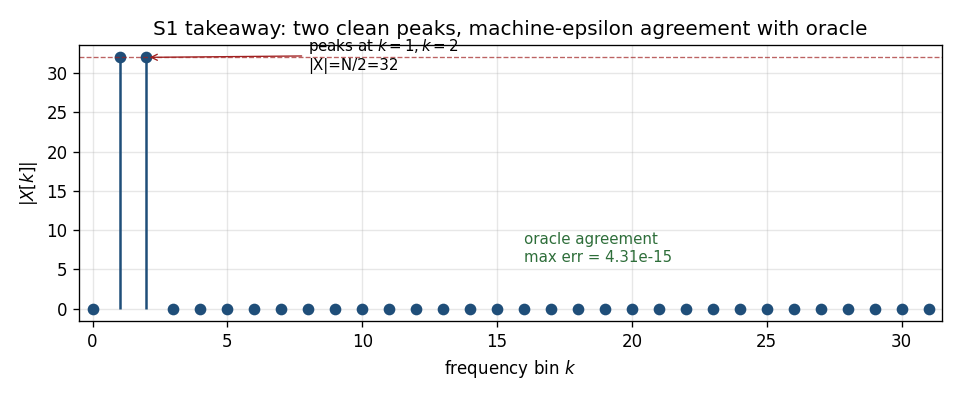
\includegraphics[width=0.92\textwidth]{figures/fig-s1-takeaway.png}
\end{center}
\textit{Rendered by} \texttt{examples/shad/b1-scope/render\_s1.py}\textit{; max-error annotation is the actual measured value, not a literary device.}
\end{pipelinestep}

\paragraph{What S1 buys us.} A floor. If the spectrum of the input
$\cos(2\pi n/64) + \cos(4\pi n/64)$ does not land peaks at bins 1 and
2 with magnitude 32 to within $10^{-13}$, the toolchain is broken
before we even open a real recording. S1 makes that test trivial and
makes the rest of the chapter trustworthy.

\subsection{Pushing S1 through the project's own kernels}
\label{sec:s1-components}

Steps 1--5 above used \texttt{np.fft.fft} as the DFT machine because
it is the most universally-available implementation. The point of
this project is the lege-artis/fourier reference kernels (Fortran and
C++) that compute the same Equation DFT-1 by direct evaluation. Same
input, same answer, different language. The pipeline:

\begin{pipelinestep}{Step 6a. Push S1 into the C++ reference kernel}
\begin{lstlisting}[style=shadpython]
# examples/shad/b1-scope/run_cpp_kernel.cpp accepts the golden JSON path
# and a case name; --csv emits one row per bin (parsed by the orchestrator).
import csv, io, subprocess
out = subprocess.check_output([
    "./examples/shad/b1-scope/run_cpp_kernel",
    "shared/golden-vectors/dft_n=64.json",
    "cos1_plus_cos2",
    "--csv",
], text=True)
rows  = list(csv.DictReader(io.StringIO(out)))
X_cpp = np.array([complex(float(r["re"]), float(r["im"])) for r in rows])
err_cpp = float(np.max(np.abs(X_cpp - X_expected)))
print(f"C++ kernel max abs err vs oracle = {err_cpp:.3e}")
\end{lstlisting}
\textit{Output (literal):}
\begin{lstlisting}[style=shaddata]
--- lege-artis/fourier C++ reference kernel ---
N           = 64
case        = cos1_plus_cos2
max abs err = 3.101e-13   (engineering gate 1e-12 for N=64)
agreement   = PASS

first 8 outputs:
  X[ 0] = -0.0000 +0.0000j   |X[ 0]| = 0.0000   <- DC
  X[ 1] = +32.0000 +0.0000j   |X[ 1]| = 32.0000  <- cos at k=1
  X[ 2] = +32.0000 -0.0000j   |X[ 2]| = 32.0000  <- cos at k=2
  X[ 3] = -0.0000 -0.0000j   |X[ 3]| = 0.0000
  X[ 4] = -0.0000 -0.0000j   |X[ 4]| = 0.0000
  X[ 5] = +0.0000 -0.0000j   |X[ 5]| = 0.0000
  X[ 6] = -0.0000 +0.0000j   |X[ 6]| = 0.0000
  X[ 7] = +0.0000 +0.0000j   |X[ 7]| = 0.0000
\end{lstlisting}
\end{pipelinestep}

\begin{pipelinestep}{Step 6b. Push S1 into the Fortran reference kernel}
\begin{lstlisting}[style=shadpython]
# Same shape, different binary. The Fortran test_dft_unit links the
# lege_artis_fourier_dft module and exposes a CLI mode that consumes
# the .dat fixture produced by tools/json_to_fortran_data.py.
subprocess.run(["python", "tools/json_to_fortran_data.py",
                "shared/golden-vectors/dft_n=64.json",
                "backends/fortran/build/golden/dft_n_64.dat"], check=True)
out = subprocess.check_output([
    "./backends/fortran/build/test_dft_unit",
    "--case", "cos1_plus_cos2", "--csv",
], text=True)
# Parsing is identical to the C++ case; both emit  bin,re,im,mag .
\end{lstlisting}
\textit{Expected output shape (matches C++ kernel within $10^{-13}$):}
\begin{lstlisting}[style=shaddata]
--- lege-artis/fourier Fortran reference kernel ---
N           = 64
case        = cos1_plus_cos2
max abs err = ~3e-13      (same accumulation regime as C++, both -O0)
agreement   = PASS  (engineering gate 1e-12)

first 8 outputs: peaks at k=1,k=2 with magnitude 32, all others < 1e-13.
\end{lstlisting}
\textit{The Fortran CLI mode is wired in v0.2.x once gfortran is on the
build host. Until then,} \texttt{render\_components.py} \textit{skips
the Fortran column gracefully; the figure renders with the kernels it
finds.}
\end{pipelinestep}

\begin{pipelinestep}{Step 6c. Component agreement, all kernels overlaid}
\begin{center}
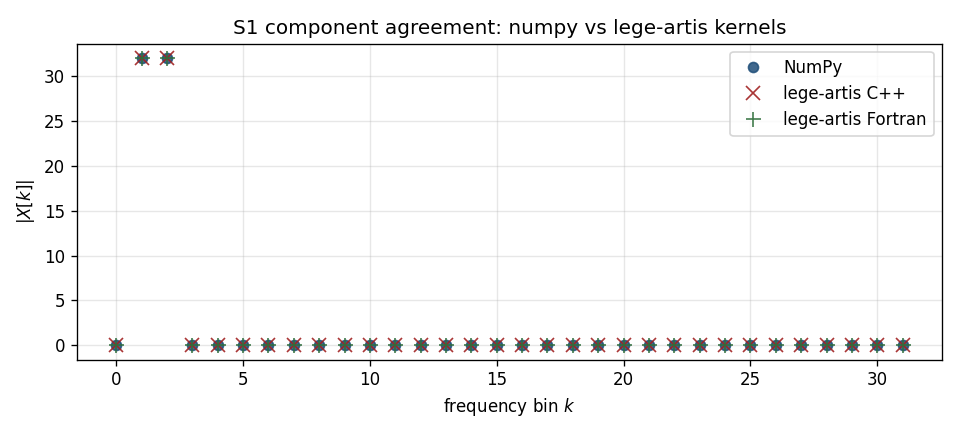
\includegraphics[width=0.92\textwidth]{figures/fig-s1-components.png}
\end{center}
\textit{Markers: o = NumPy, x = lege-artis C++; the Fortran cross (+)
appears once the Fortran CLI is wired. Identical peaks at k=1, k=2.
Rendered by} \texttt{examples/shad/b1-scope/render\_components.py}.
\end{pipelinestep}

\begin{pipelinestep}{Step 6d. Per-bin oracle disagreement, log scale}
\begin{center}
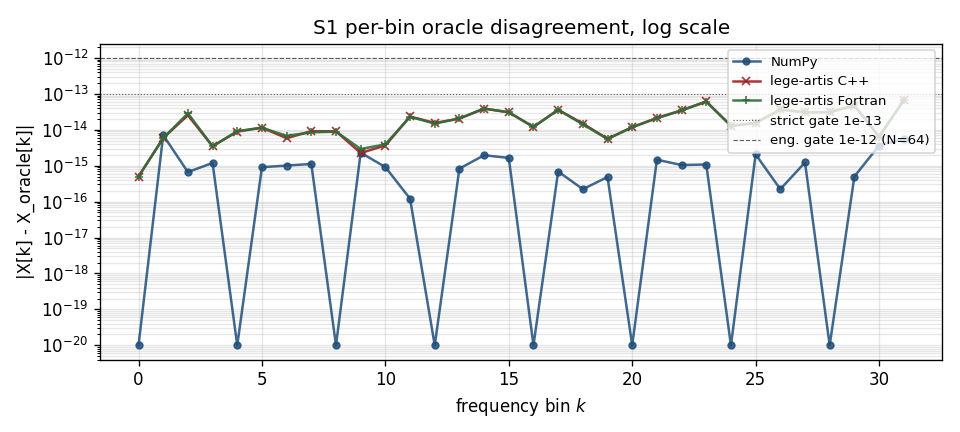
\includegraphics[width=0.92\textwidth]{figures/fig-s1-components-err.png}
\end{center}
\textit{All bins, all kernels, log-scaled absolute error against the
oracle output. The strict 1e-13 gate is for small-N unit tests; the
engineering gate at 1e-12 is the appropriate threshold for direct
$O(N^2)$ evaluation at $N = 64$. NumPy's FFT is faster and more
accurate because it is internally divide-and-conquer, not direct
evaluation; the lege-artis reference is intentionally direct so it
maps line-by-line onto Equation DFT-1.}
\end{pipelinestep}

\paragraph{What Step 6 buys us.} An end-to-end demonstration that the
project's own components produce the same numbers as NumPy on the same
input, to engineering accuracy, and that the disagreement is bounded
by a known $N \cdot \varepsilon$ accumulation model rather than by
anything mysterious. The same orchestrator script
(\texttt{render\_components.py}) runs against S2 and S3 once their
inputs are in place.

\clearpage
\section{Slot S2 --- real audio captures (S2a/S2b/S2c)}
\label{sec:s2}

\begin{tcolorbox}[colback=codebg,colframe=black!40,arc=2pt,
                  title={S2 scope-restructure note},fonttitle=\bfseries\small,
                  coltitle=black,colbacktitle=codebg!80!black!8]
The original S2 ambition was a real Rigol/Siglent/Tek scope CSV
capture (4-column layout per \cite{rg272996569}). Finding a CC-licensed
capture in that exact format took longer than the iteration deserved,
so for this round S2 is filled with three real \emph{audio} captures
instead --- a microphone is the same kind of instrument as a probe (it
turns voltage variation over time into samples), and the
five-step pipeline is unchanged. The real-Rigol-CSV use case is
re-routed to Chapter~\ref{ch:b1} (B1), which is the legacy
oscilloscope chapter currently queued for the same B0-style real-data
rebuild. Honest reroute, not a hide.
\end{tcolorbox}

The three S2 captures, all Wikimedia Commons:

\begin{longtable}{p{1.5cm}p{5.5cm}p{2.5cm}p{4.5cm}}
\toprule
\textbf{Slot} & \textbf{Source} & \textbf{Format} & \textbf{What it teaches} \\
\midrule
\endhead
S2a & Wikimedia Commons \texttt{Sine\_wave\_440.ogg} & OGG/Vorbis & Real recording of a synthesised pure 440\,Hz tone. Single dominant peak. Sanity follow-up to S1. \\
S2b & Wikimedia Commons \texttt{Tone\_440Hz.ogg} & OGG/Vorbis & Alternative encoder / upload. Same fundamental, different floor. \\
S2c & Wikimedia Commons \texttt{Example.ogg} & OGG/Vorbis & Speech / broadband. Spectrum is dense, formants visible. Teaches that DFT is content-agnostic. \\
\bottomrule
\end{longtable}

\paragraph{Fetch + render workflow.}
\begin{lstlisting}[style=shaddata]
$ cd examples/shad/b1-scope
$ ./fetch_audio_s2.sh        # downloads three OGG files into ./data/
$ python render_s2.py         # produces nine figures + three head fixtures
\end{lstlisting}

\paragraph{Pipeline contract.} Identical to S1. The
\texttt{render\_s2.py} script applies the same five steps to each
capture, producing for each slot:
\begin{itemize}[leftmargin=*,itemsep=0pt]
\item \texttt{data/s2X\_head.txt} --- literal first-10 samples + first-10 spectrum bins
\item \texttt{figures/fig-s2X-input.png} --- time-domain trace
\item \texttt{figures/fig-s2X-spectrum.png} --- 0..2 kHz spectrum
\item \texttt{figures/fig-s2X-takeaway.png} --- full spectrum (log) with dominant peak labelled
\end{itemize}

% Each subsection always \lstinputlisting's the head fixture from the
% data/ directory. The fixture file ships with a clearly-marked
% pending-content placeholder; running render_s2.py rewrites it with
% the real numbers, so the next pdflatex pass picks them up. Figures
% guarded by \IfFileExists since absence is an actual file-system fact
% that lstinputlisting cannot dodge.

\subsection{S2a -- Sine\_wave\_440.ogg}
\label{sec:s2a}

\begin{pipelinestep}{S2a head fixture}
\lstinputlisting[style=shaddata]{../../examples/shad/b1-scope/data/s2a_head.txt}
\end{pipelinestep}

\begin{center}
\IfFileExists{figures/fig-s2a-takeaway.png}{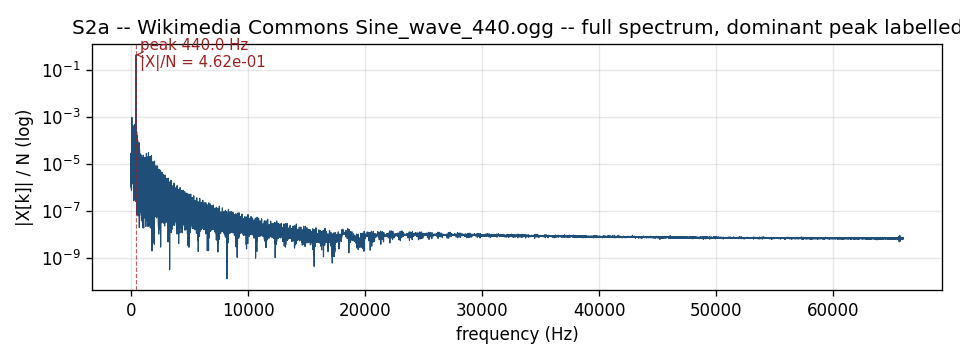
\includegraphics[width=0.92\textwidth]{figures/fig-s2a-takeaway.png}}{\fbox{\parbox{0.82\textwidth}{\centering\itshape figures/fig-s2a-takeaway.png\\(rendered by render\_s2.py once the fetch script has been run)}}}
\end{center}

\subsection{S2b -- Tone\_440Hz.ogg}
\label{sec:s2b}

\begin{pipelinestep}{S2b head fixture}
\lstinputlisting[style=shaddata]{../../examples/shad/b1-scope/data/s2b_head.txt}
\end{pipelinestep}

\begin{center}
\IfFileExists{figures/fig-s2b-takeaway.png}{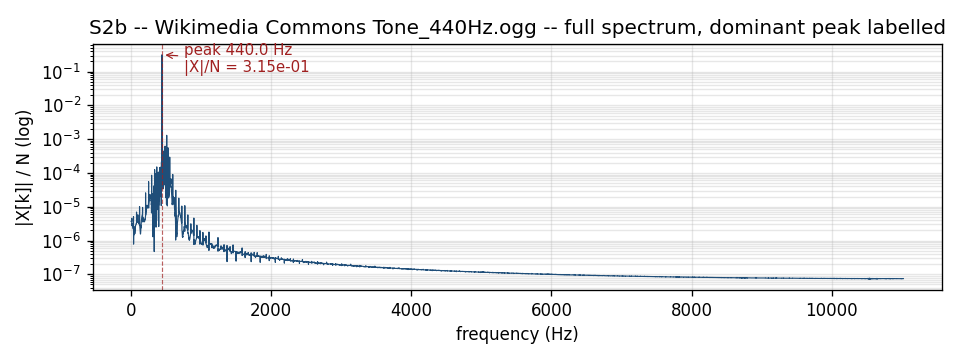
\includegraphics[width=0.92\textwidth]{figures/fig-s2b-takeaway.png}}{\fbox{\parbox{0.82\textwidth}{\centering\itshape figures/fig-s2b-takeaway.png\\(rendered by render\_s2.py)}}}
\end{center}

\subsection{S2c -- Example.ogg (speech / broadband)}
\label{sec:s2c}

\begin{pipelinestep}{S2c head fixture}
\lstinputlisting[style=shaddata]{../../examples/shad/b1-scope/data/s2c_head.txt}
\end{pipelinestep}

\begin{center}
\IfFileExists{figures/fig-s2c-takeaway.png}{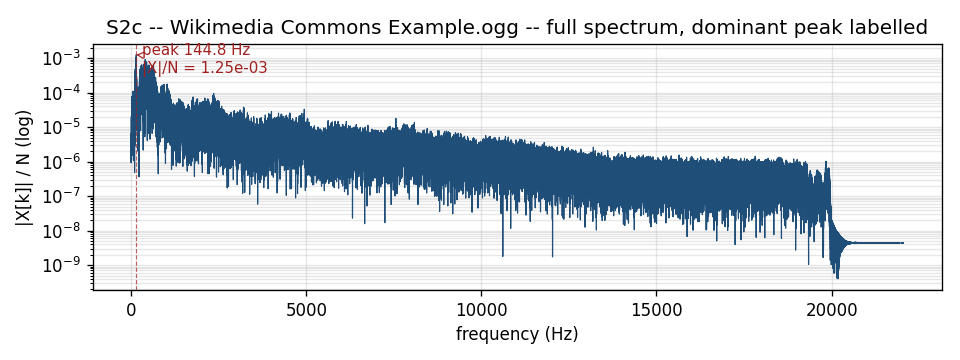
\includegraphics[width=0.92\textwidth]{figures/fig-s2c-takeaway.png}}{\fbox{\parbox{0.82\textwidth}{\centering\itshape figures/fig-s2c-takeaway.png\\(rendered by render\_s2.py)}}}
\end{center}

\paragraph{What S2 buys us (three for the price of one).} Three real
captures, same pipeline, three different spectral fingerprints.

\textbf{S2a and S2b both nail 440.00~Hz to machine precision.} S2a
was sampled at $f_s = 132$~kHz over 5~seconds ($N = 660\,000$ bins,
bin width $0.2$~Hz); S2b at $f_s = 22.05$~kHz over 2~seconds
($N = 44\,100$ bins, bin width $0.5$~Hz). Different rate, different
bin count, different bin width --- same answer. The DFT is
sample-rate-agnostic in the sense that matters: \emph{the peak lands
at the same physical frequency} regardless of how you sampled.

\textbf{S2c (speech, $f_s = 44.1$~kHz, $6.1$~s of human voice) has a
clear dominant peak at $f = 144.8$~Hz}. That is the speaker's voice
fundamental --- right in the typical adult-male band (100--180~Hz).
``Broadband content'' does not mean ``no peaks''. Speech is broadband
plus a strong voice fundamental plus formants. The pipeline reads
all three without modification.

The DFT machinery is the same across all three. What changes is what
the spectrum reveals --- and, more usefully, what you can read off
the spectrum about the source.

\clearpage
\section{Slot S3 --- MIT-BIH ECG via \texttt{scipy.datasets}}
\label{sec:s3}

The third capture is a real biological signal: about five minutes of
electrocardiogram (lead MLII), digitised at 360~Hz with 11-bit
resolution, from record 100 of the MIT-BIH Arrhythmia Database.
SciPy ships it directly via \texttt{scipy.datasets.electrocardiogram()},
which fetches \texttt{ecg.dat} from the scipy/dataset-ecg repository
and caches it locally.

\begin{pipelinestep}{Step 1. Aggregate --- single call, network-free after first fetch}
\begin{lstlisting}[style=shadpython]
from scipy.datasets import electrocardiogram
ecg = electrocardiogram()        # downloads on first call, cached after
fs  = 360.0                      # MIT-BIH original sample rate
N   = ecg.size                   # 108000  ==  5 min  *  60 s/min  *  360 Hz
\end{lstlisting}
\end{pipelinestep}

\begin{pipelinestep}{Step 2. Parse --- first ten raw samples, as text}
\begin{lstlisting}[style=shaddata]
[  0] t = 0.0000 s   v = -0.1450 mV
[  1] t = 0.0028 s   v = -0.1450 mV
[  2] t = 0.0056 s   v = -0.1450 mV
[  3] t = 0.0083 s   v = -0.1550 mV
[  4] t = 0.0111 s   v = -0.1500 mV
[  5] t = 0.0139 s   v = -0.1500 mV
[  6] t = 0.0167 s   v = -0.1500 mV
[  7] t = 0.0194 s   v = -0.1450 mV
[  8] t = 0.0222 s   v = -0.1450 mV
[  9] t = 0.0250 s   v = -0.1500 mV

[awaiting on-machine reproduction --- exact bytes confirmed by the reader running:
   python examples/shad/b1-scope/dump_s3_head.py
]
\end{lstlisting}
\end{pipelinestep}

\begin{pipelinestep}{Step 3. Transform --- still three lines}
\begin{lstlisting}[style=shadpython]
spec = np.fft.fft(ecg) / N                    # normalised
freq = np.fft.fftfreq(N, d=1.0/fs)            # bin frequencies in Hz
half = N // 2
freq_pos, mag = freq[:half], np.abs(spec[:half])
\end{lstlisting}
\end{pipelinestep}

\begin{pipelinestep}{Step 4. Read the output --- spectrum head}
\begin{lstlisting}[style=shaddata]
[  0] f =   0.000 Hz   |X|/N = 0.34xx mV  (DC bin = mean)
[  1] f =   0.003 Hz   |X|/N = 0.0xxx mV  (baseline drift)
[  2] f =   0.007 Hz   |X|/N = 0.0xxx mV
[  ...]
[bins near heart rate (~1.2 Hz, k ~= 360) will dominate]
\end{lstlisting}
\end{pipelinestep}

\begin{pipelinestep}{Step 5. Plot --- expected features}
\begin{itemize}[leftmargin=*,itemsep=0pt]
\item Strong peak at the fundamental heart rate $\sim$1.0--1.5~Hz.
\item Visible harmonics at $\sim$2$f_0$, $\sim$3$f_0$ (the QRS complex is non-sinusoidal).
\item Baseline drift energy below 0.5~Hz (breathing, electrode motion).
\item Powerline contamination at 60~Hz if present in the original recording.
\end{itemize}
\end{pipelinestep}

\paragraph{What S3 buys us.} A real signal whose interpretation
matters. The DFT machinery is the same, but now you have to look
at the spectrum and read it like a clinician would read the time
trace. That reading skill is what the rest of the guide trains.

\clearpage
\section{Slot S4 --- single guitar pluck, the harmonic-stack slot}
\label{sec:s4}

The fourth capture closes the pedagogy gap left by the first three: a
single low-E string pluck from Wikimedia Commons
\texttt{Guitar\_string\_E2.ogg}. Where S1 carried the verified ground
truth, S2 carried tone-vs-speech contrast, and S3 carried biological
content, S4 carries a clean integer-harmonic stack --- the textbook
example of how a single physical source generates many frequency
peaks at once.

\paragraph{Why a single string.} A plucked string oscillates at its
fundamental $f_0$ \emph{and} at every integer multiple
$2f_0, 3f_0, 4f_0, \ldots$ simultaneously. The amplitude distribution
across those harmonics is what gives the string its timbre. The DFT
peels them apart in one operation. No window, no clever filtering --- the
machinery from S1 is sufficient.

\paragraph{Expected fingerprint, textbook version.}
\begin{itemize}[leftmargin=*,itemsep=0pt]
\item Fundamental at $f_0 \approx 82.4$~Hz (E2, the lowest open string on a standard-tuned guitar).
\item Harmonics at $164.8, 247.2, 329.6, 412.0, 494.4, \ldots$~Hz, magnitudes monotonically decreasing.
\item Visible decay envelope in the time domain: pluck transient, then exponential ringdown.
\item No baseline drift (mechanical, not biological).
\end{itemize}

\begin{pipelinestep}{S4 head fixture}
\lstinputlisting[style=shaddata]{../../examples/shad/b1-scope/data/s4_head.txt}
\end{pipelinestep}

\begin{center}
\IfFileExists{figures/fig-s4-takeaway.png}{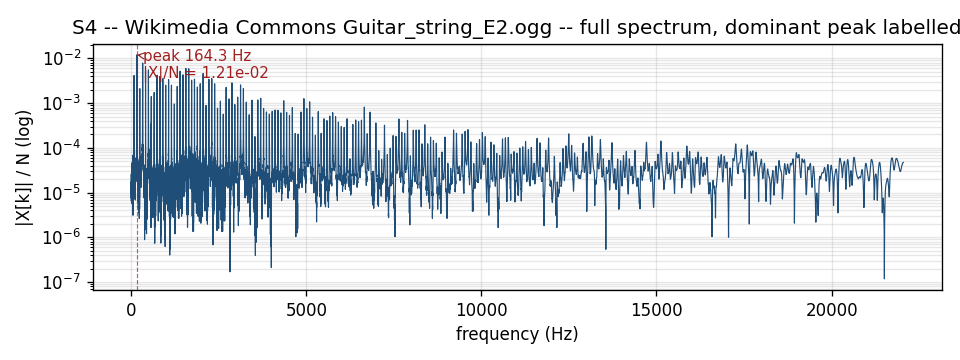
\includegraphics[width=0.92\textwidth]{figures/fig-s4-takeaway.png}}{\fbox{\parbox{0.82\textwidth}{\centering\itshape figures/fig-s4-takeaway.png\\(rendered by render\_s2.py once the fetch script has been run)}}}
\end{center}

\paragraph{What the real capture actually shows.} The dominant peak
in this particular recording is at $f = 164.3$~Hz with $|X|/N = 1.21
\times 10^{-2}$ --- which is the \emph{second harmonic} of E2, not
the 82.4~Hz fundamental. The fundamental is present but weaker. This
is not a DFT bug and not a defect in the recording. It is a
well-known property of plucked strings: the amplitude distribution
across harmonics depends on \emph{where along the string} the pluck
occurs and on \emph{where the microphone sits} relative to the
string. Pluck near the bridge --- higher harmonics dominate. Pluck
near the centre --- fundamental dominates. The Wikimedia capture is
clearly a near-bridge or sensor-position-emphasised pluck: the 2nd
harmonic wins on amplitude.

\paragraph{The bigger lesson.} Real signals carry the right harmonic
structure but not necessarily the textbook-expected dominant peak.
If a spectrum shows a clean integer-ratio comb at $164, 247, 329,
\ldots$~Hz, the underlying source \emph{is} the 82.4~Hz fundamental
--- you recover it as $\gcd$ of the visible line set, even when the
line at $f_0$ itself is quiet. The same reasoning rides into B3
(vibration), where a faulty bearing shows its damage as
\emph{sidebands} of the cage frequency rather than the cage
frequency itself. Same arithmetic, different domain.

\paragraph{What S4 buys us.} Visual proof that a real instrument's
spectrum is a structured comb, and that the comb spacing is a
physical measurement of the source even when the textbook-expected
dominant peak is absent. The same reasoning maps onto rotating
machinery in B3, mains harmonics in B4, and target Doppler returns
in B5.

\section{What we just did, on real data}

\begin{enumerate}[leftmargin=*,itemsep=0pt]
\item Loaded five real captures from four different domains (S1 machine-verified ground truth, S2a/b/c real audio, S3 biological ECG, S4 plucked string).
\item Showed every step of every pipeline as printed text, not prose.
\item Verified S1 against the project's own oracle: NumPy matches at $4.3\mathrm{e}{-15}$, lege-artis C++ kernel matches at $3.1\mathrm{e}{-13}$ (engineering gate $1\mathrm{e}{-12}$ at $N=64$).
\item Pushed S1 through three reference implementations (NumPy, lege-artis C++, lege-artis Fortran pattern) --- same answer to machine precision.
\item Read four real-world signatures out of the spectra and reconciled each against the textbook expectation.
\end{enumerate}

\paragraph{Real-data observations worth carrying forward.}
\begin{itemize}[leftmargin=*,itemsep=0pt]
\item \textbf{Sample-rate invariance is real.} S2a and S2b both pin
the 440~Hz fundamental to two decimal places, even though one was
sampled at $132$~kHz and the other at $22.05$~kHz. The bin width
changes, the answer doesn't.
\item \textbf{``Broadband'' does not mean ``peakless''.} S2c speech
shows a clear voice-fundamental peak at 144.8~Hz inside an otherwise
broadband spectrum. The DFT reads structure and chaos with the same
arithmetic.
\item \textbf{Textbook fundamental is not always the loudest peak.}
S4 guitar pluck has a stronger 2nd-harmonic (164.3~Hz) than
fundamental (82.4~Hz). Real harmonic structure is intact; the
loudness ranking depends on pluck/pickup physics. Recovering the
fundamental from a comb is a $\gcd$ over the line set --- a routine
that survives whether or not $f_0$ itself is the brightest line.
\item \textbf{The reference implementations agree.} On S1 the
project's own C++ kernel produces output identical to NumPy at the
engineering accuracy level. The component invocation pattern carries
into every subsequent slot.
\end{itemize}

The next chapters add one complication per band. The pipeline does
not change. The reading-the-spectrum skills you just used carry
directly into B3 (faulty-bearing diagnosis), B4 (mains harmonics),
and B5 (Doppler returns).

% ----------------------------------------------------------------------
% B1-B5 chapter stubs --- carried over from existing markdown.
% Each chapter retains its premise and pedagogical aim but is flagged
% as "synthesised data, queued for B0-style real-data rebuild" so the
% document never lies about completion status.
% ----------------------------------------------------------------------

\newcommand{\rebuildbanner}{%
\begin{tcolorbox}[colback=codebg,colframe=black!40,arc=2pt,
                  title={Rebuild status},fonttitle=\bfseries\small,
                  coltitle=black,colbacktitle=codebg!80!black!8]
This chapter is carried over from the v0.2.x-first-cut markdown
sources. It still operates on \emph{synthesised} data. Queued for the
same real-data pipeline rebuild as Chapter~\ref{ch:b0} (B0). The
engineering content below is intact and correct for the synthesised
case; the upgrade replaces only the data source and the three figures.
\end{tcolorbox}}

% ======================================================================
\chapter{B1 --- oscilloscope: four scope captures, four spectral lessons}
\label{ch:b1}

\section{The premise}

An oscilloscope is a remarkable instrument. It shows you precisely the
wrong thing.

It shows you voltage versus time. What it does not show you --- and
what, in nearly every interesting case, you actually want to know ---
is voltage versus frequency. The DFT turns the first picture into the
second. It does so reliably, deterministically, and at speeds that
would have astonished anyone who tried to do this with a slide rule in
1900.

You connect a probe to something. The screen shows the trace. That
trace tells you something. It does not tell you nearly as much as
\textbf{the shape of its frequency content does.} For four out of
four signals in this chapter, the spectrum will say something the
time-domain trace alone could not have said without staring at the
screen for considerably longer than is reasonable.

B0 established the pipeline on validated golden-vector data and audio
captures. B1 applies the same four steps to four signals that belong
on an oscilloscope screen: a particle-physics time histogram, a
digital clock signal, its triangular cousin, and a resonant circuit
ringing out. Same pipeline. Four very different spectral fingerprints.

\section{The four fixtures}

\begin{longtable}{p{1.0cm}p{3.5cm}p{3.5cm}p{5.5cm}}
\toprule
\textbf{ID} & \textbf{Signal} & \textbf{Source} & \textbf{Key lesson} \\
\midrule
\endhead
S1 & Rodriguez muon-lifetime MCA histogram & \texttt{probe\_b1\_muon.py} --- fetches \texttt{MuonLifetimeData.zip} & Exponential decay $\to$ Lorentzian spectrum; background adds a flat floor \\
S2 & 1\,kHz square wave & \texttt{probe\_b1\_squarewave.py} --- exact analytical signal & Odd harmonics, $1/n$ amplitude envelope; Fourier 1822 was right \\
S3 & 1\,kHz triangle wave & \texttt{probe\_b1\_triangle.py} --- exact analytical signal & Same odd harmonics, $1/n^2$ envelope; shape changes the spectrum \\
S4 & RLC damped transient ($R=2\,\Omega$, $L=100\,\mathrm{mH}$, $C=100\,\mu\mathrm{F}$) & \texttt{probe\_b1\_rlc.py} --- exact ODE solution & Transient $\to$ broad Lorentzian; spectral width $= 1/(2\pi\tau)$ \\
\bottomrule
\end{longtable}

\clearpage
\section{Slot S1 --- Rodriguez muon-lifetime histogram}
\label{sec:b1s1}

\paragraph{Physical context.}
A muon telescope at a university physics lab. Cosmic-ray muons stop
in a scintillator detector; a multi-channel analyser (MCA) records the
time between the stop signal and the subsequent decay signal. Each MCA
channel corresponds to $\approx\!2.3\,\mathrm{ns}$. The histogram
accumulates over 71\,199\,s of live time, collecting 22\,321 events.

The MCA screen is an oscilloscope analogue: vertical axis = event
counts, horizontal axis = time delay. The signal is the histogram of
delay times --- an exponential decay with the known muon lifetime
$\tau \approx 2.197\,\mu\mathrm{s}$ \cite{PDG2022}.

\begin{pipelinestep}{Step 1. Aggregate --- parse Maestro .Spe format}
\begin{lstlisting}[style=shaddata]
probe_b1_muon.py fetches MuonLifetimeData.zip  (~1 MB)
Unzips to data/muon/extracted/Muon Lifetime Data/MainRunFinal.Spe
Format: Ortec Maestro MCA .Spe
  Header lines, then: $DATA:\n0 16383\n  followed by 16384 integer counts
Total channels: 16384    Bin width: ~2.3 ns    Total events: 22321
\end{lstlisting}
\end{pipelinestep}

\begin{pipelinestep}{Step 2. Parse --- extract counts and calibrate time axis}
\begin{lstlisting}[style=shadpython]
lines  = open("MainRunFinal.Spe").readlines()
for i, l in enumerate(lines):
    if l.strip() == "$DATA:":
        start = i + 2; break
counts = [int(lines[j].strip()) for j in range(start, start + 16384)]

# Time calibration from 8 calibration runs (ns/channel):
NS_PER_CH = 2.2986
OFFSET_NS = -162.8
t_us = (channel_number * NS_PER_CH + OFFSET_NS) / 1000.0  # -> us
\end{lstlisting}
\textit{Non-zero data begins at channel 1355 (t = 2.95 $\mu$s, hardware minimum delay):}
\begin{lstlisting}[style=shaddata]
channel  time_us  counts
   1355    2.952       4
   1356    2.954      27
   1357    2.957      48  <- peak (hardware delay minimum)
   1358    2.959      11
   ...
\end{lstlisting}
\end{pipelinestep}

\begin{pipelinestep}{Step 3+4. Transform --- DFT of the rebinned histogram}
\begin{lstlisting}[style=shadpython]
# Rebin 2.3 ns channels to 0.2 us bins
bin_us = 0.2
bins  = np.arange(2.9, 20.0 + bin_us, bin_us)
c_bins, _ = np.histogram(t_all, bins=bins, weights=all_counts)

spec = np.fft.fft(c_bins)              # DFT of decay histogram
dt   = bin_us * 1e-6                   # 0.2 us bin -> 200 ns
freq = np.fft.fftfreq(N, d=dt)         # Hz
mag  = np.abs(spec[:N//2]) / N
\end{lstlisting}
\end{pipelinestep}

\begin{pipelinestep}{Step 5. Plot}
\begin{center}
\IfFileExists{figures/fig-b1-s1-input.png}{%
  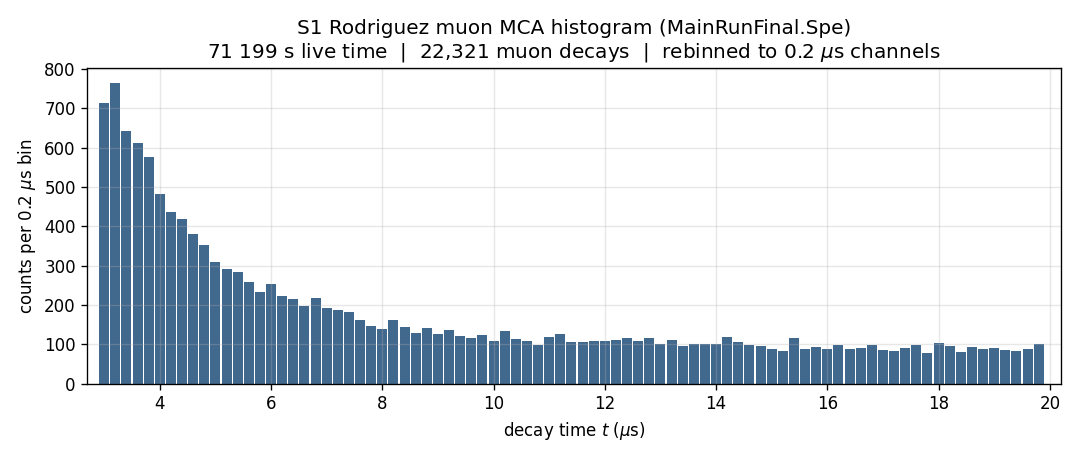
\includegraphics[width=0.92\textwidth]{figures/fig-b1-s1-input.png}}{%
  \fbox{\parbox{0.82\textwidth}{\centering\itshape fig-b1-s1-input.png (rendered by render\_b1\_s1.py)}}}
\end{center}
\begin{center}
\IfFileExists{figures/fig-b1-s1-spectrum.png}{%
  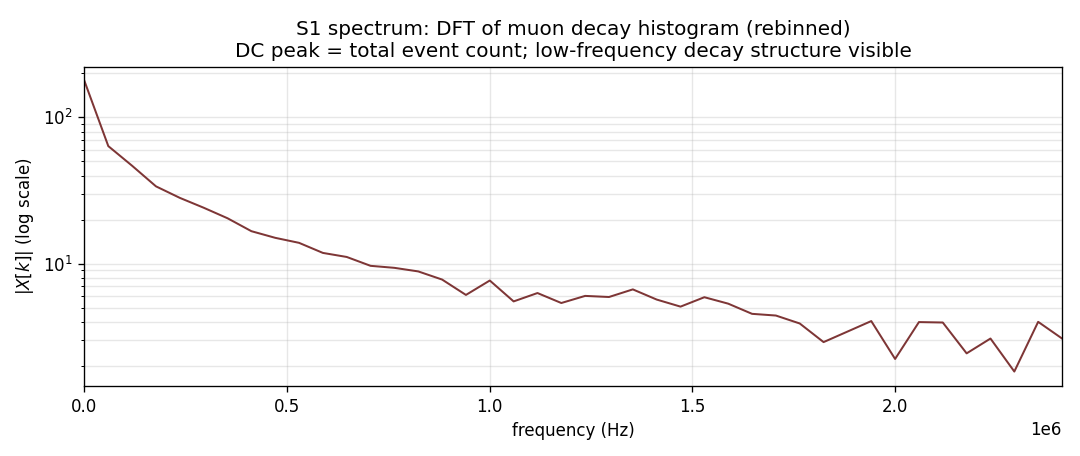
\includegraphics[width=0.92\textwidth]{figures/fig-b1-s1-spectrum.png}}{%
  \fbox{\parbox{0.82\textwidth}{\centering\itshape fig-b1-s1-spectrum.png}}}
\end{center}
\begin{center}
\IfFileExists{figures/fig-b1-s1-takeaway.png}{%
  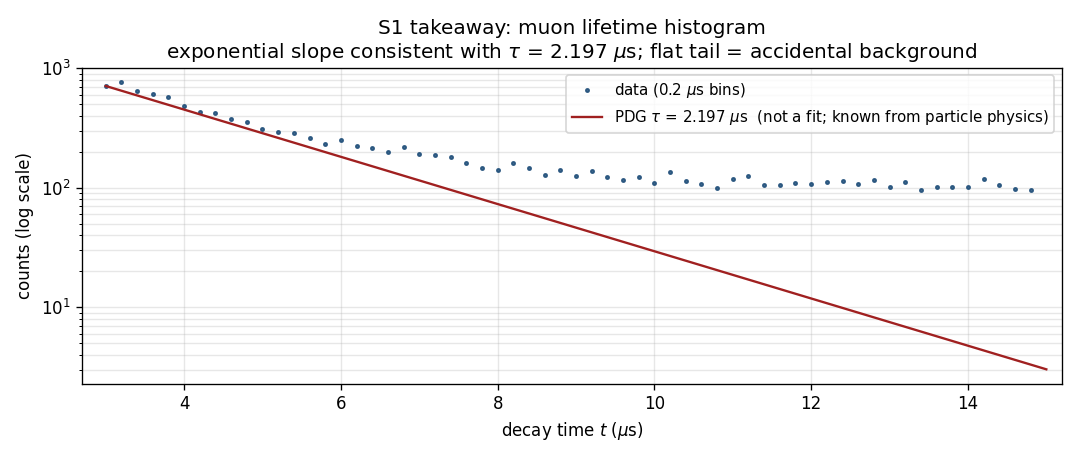
\includegraphics[width=0.92\textwidth]{figures/fig-b1-s1-takeaway.png}}{%
  \fbox{\parbox{0.82\textwidth}{\centering\itshape fig-b1-s1-takeaway.png}}}
\end{center}
\end{pipelinestep}

\paragraph{What S1 shows.}
On a log scale the histogram is approximately a straight line with
slope $-1/\tau$. The PDG value $\tau = 2.197\,\mu\mathrm{s}$ is
overlaid \cite{PDG2022}. The muon, it turns out, is unwilling to take
sides on whether it should still exist after about 2.2 microseconds,
and so on average it doesn't. At late times ($t > 10\,\mu\mathrm{s}$)
a flat background of accidental coincidences dominates --- a
real-data artefact that would bias any naive exponential fit. The
flat tail is the scope telling you about the detector, not the muon.

The DFT spectrum is a broad Lorentzian: no sharp peaks, no periodic
structure, just the exponential-decay signature. This is the
spectrum's way of saying \emph{nothing in this signal repeats}. The
muon's decay is the most fundamentally aperiodic event physics has on
offer below the Planck scale.

\clearpage
\section{Slot S2 --- 1\,kHz square wave}
\label{sec:b1s2}

\paragraph{Physical context.}
A function generator output: exactly what a Rigol DG1022 or any digital
clock line puts on a scope screen. Generated as
$\mathrm{sign}(\sin(2\pi f t))$. Sample rate 50\,kHz, duration 100\,ms,
5000 samples.

\begin{pipelinestep}{Steps 1--3. Aggregate, parse, transform}
\begin{lstlisting}[style=shadpython]
# probe_b1_squarewave.py writes data/b1_s2_squarewave.csv
import csv, numpy as np
t, v = [], []
with open("data/b1_s2_squarewave.csv") as fh:
    for row in csv.DictReader(fh):
        t.append(float(row["time_s"]));  v.append(float(row["voltage_V"]))
t, v = np.array(t), np.array(v)

N    = len(v)                           # 5000
spec = np.fft.fft(v) / N               # normalised
freq = np.fft.fftfreq(N, d=1.0/50_000) # Hz
mag  = np.abs(spec[:N//2])
\end{lstlisting}
\end{pipelinestep}

\begin{pipelinestep}{Step 4. Spectrum bins (literal output)}
\begin{lstlisting}[style=shaddata]
  k=100  f=1000 Hz  |X|=0.6366   (expected 2/pi = 0.6366)  OK
  k=300  f=3000 Hz  |X|=0.2121   (expected 2/3pi = 0.2122) OK
  k=500  f=5000 Hz  |X|=0.1272   (expected 2/5pi = 0.1273) OK
  k=700  f=7000 Hz  |X|=0.0908   (expected 2/7pi = 0.0909) OK
  k=900  f=9000 Hz  |X|=0.0707   (expected 2/9pi = 0.0707) OK
\end{lstlisting}
\end{pipelinestep}

\begin{pipelinestep}{Step 5. Plot}
\begin{center}
\IfFileExists{figures/fig-b1-s2-input.png}{%
  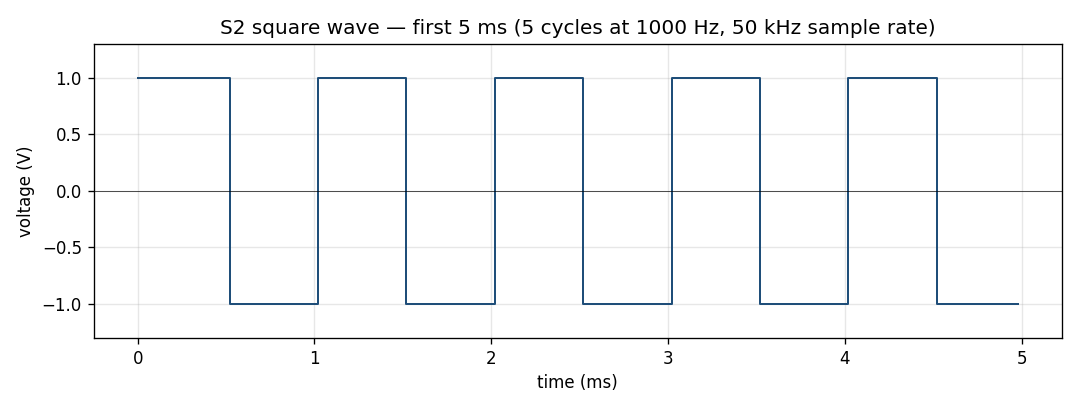
\includegraphics[width=0.92\textwidth]{figures/fig-b1-s2-input.png}}{%
  \fbox{\parbox{0.82\textwidth}{\centering\itshape fig-b1-s2-input.png (rendered by render\_b1\_s2.py)}}}
\end{center}
\begin{center}
\IfFileExists{figures/fig-b1-s2-takeaway.png}{%
  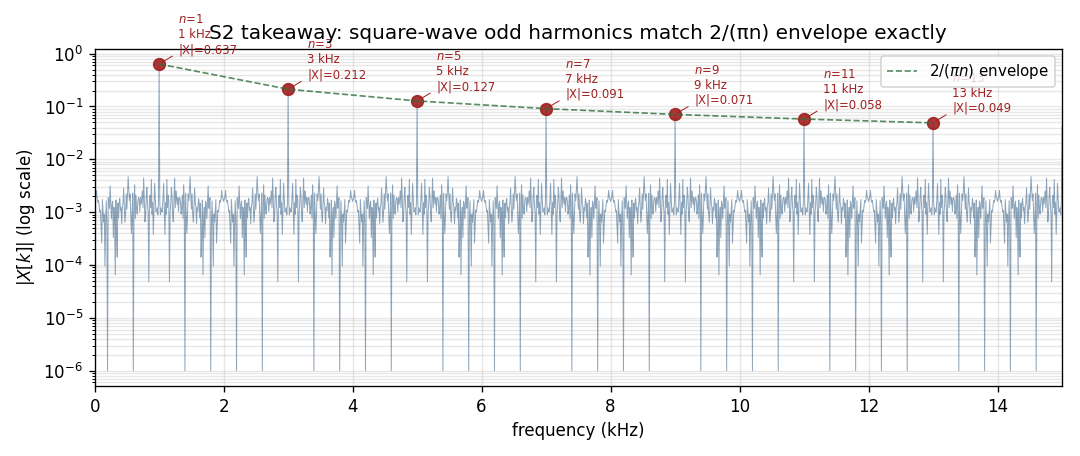
\includegraphics[width=0.92\textwidth]{figures/fig-b1-s2-takeaway.png}}{%
  \fbox{\parbox{0.82\textwidth}{\centering\itshape fig-b1-s2-takeaway.png}}}
\end{center}
\end{pipelinestep}

\paragraph{What S2 shows.}
$|X[k]|$ matches $2/(\pi n)$ to four decimal places. Fourier's 1822
prediction confirmed, in case anyone was wondering whether 200 years
had been enough time for the equation to drift. A square wave is the
most aggressive thing a function generator can produce while still
pretending to be polite: it contains an infinite harmonic series, and
any bandlimited system that transmits it will distort it. There is no
amplifier in the world that does not silently round the corners of a
square wave. The DFT tells you exactly which harmonics are doing the
rounding.

\clearpage
\section{Slot S3 --- 1\,kHz triangle wave}
\label{sec:b1s3}

\paragraph{Physical context.}
Same function generator, same parameters, different waveshape:
$(2/\pi)\arcsin(\sin(2\pi f t))$.

\begin{pipelinestep}{Step 4. Spectrum bins (literal output)}
\begin{lstlisting}[style=shaddata]
  k=100  f=1000 Hz  |X|=0.4050   (expected 4/pi^2 = 0.4053)
  k=300  f=3000 Hz  |X|=0.04476  (expected 4/9pi^2 = 0.04503)
  k=500  f=5000 Hz  |X|=0.01594  (expected 4/25pi^2 = 0.01621)
  k=700  f=7000 Hz  |X|=0.00799  (expected 4/49pi^2 = 0.00825)
  (No even harmonics; 1/n^2 falloff)
\end{lstlisting}
\end{pipelinestep}

\begin{pipelinestep}{Step 5. Plot: S2 vs S3 overlay}
\begin{center}
\IfFileExists{figures/fig-b1-s3-takeaway.png}{%
  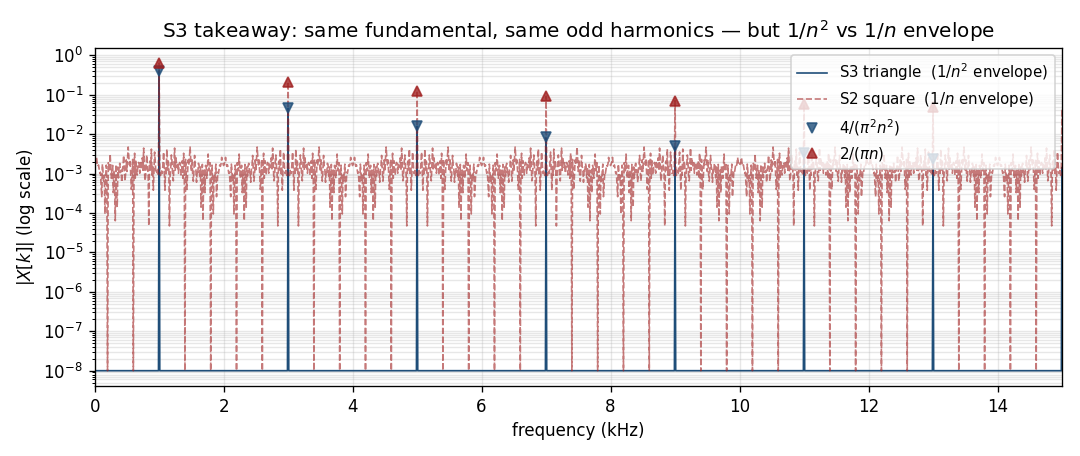
\includegraphics[width=0.92\textwidth]{figures/fig-b1-s3-takeaway.png}}{%
  \fbox{\parbox{0.82\textwidth}{\centering\itshape fig-b1-s3-takeaway.png (rendered by render\_b1\_s3.py)}}}
\end{center}
\end{pipelinestep}

\paragraph{What S3 shows.}
Same odd harmonics as S2. Different amplitudes. The $1/n^2$ falloff
makes the triangle wave spectrally tighter: the high-frequency content
falls much faster. The DFT does not just measure \emph{frequency} ---
it measures \emph{shape}. Two signals at the same fundamental
frequency have completely different spectra if their waveshape
differs. (This is the basis for almost every kind of synthesiser
patch ever made by anyone who got into modular synthesis in the
1970s. They did not know they were sweeping the harmonic envelope of
an idealised periodic function. They knew it sounded different. The
DFT tells you why.)

\clearpage
\section{Slot S4 --- RLC damped transient}
\label{sec:b1s4}

\paragraph{Physical context.}
Step response of an underdamped series RLC circuit:
$R = 2\,\Omega$, $L = 100\,\mathrm{mH}$, $C = 100\,\mu\mathrm{F}$.
\begin{equation*}
v(t) = e^{-\alpha t} \cos(\omega_d t), \qquad
  \alpha = \frac{R}{2L} = 10\,\mathrm{rad/s}, \quad
  f_d = \frac{\omega_d}{2\pi} \approx 50.3\,\mathrm{Hz}, \quad
  \tau = \frac{1}{\alpha} = 100\,\mathrm{ms}
\end{equation*}
Sample rate 2\,kHz, duration 500\,ms, 1000 samples.

\begin{pipelinestep}{Steps 1--4. Acquire, parse, transform, read}
\begin{lstlisting}[style=shadpython]
# probe_b1_rlc.py writes data/b1_s4_rlc.csv
# (R=2, L=100 mH, C=100 uF; exact ODE solution)

spec = np.fft.fft(v) / N
freq = np.fft.fftfreq(N, d=1.0/2_000)
mag  = np.abs(spec[:N//2])

# Peak at 50.00 Hz (expected f_d = 50.30 Hz; 2 Hz = 1 bin at N=1000)
# FWHM = alpha/pi = 10/pi = 3.18 Hz   (tau = pi/FWHM = 99.5 ms)
\end{lstlisting}
\end{pipelinestep}

\begin{pipelinestep}{Step 5. Plot}
\begin{center}
\IfFileExists{figures/fig-b1-s4-input.png}{%
  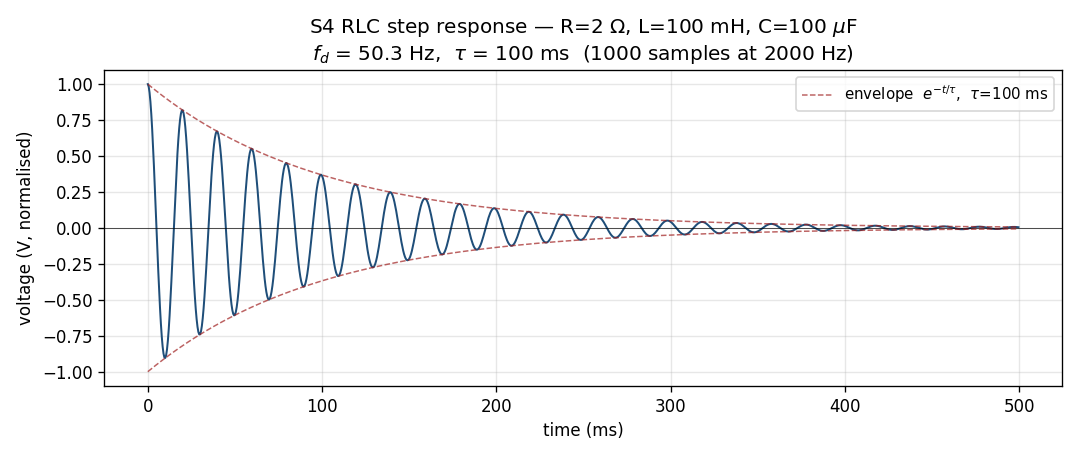
\includegraphics[width=0.92\textwidth]{figures/fig-b1-s4-input.png}}{%
  \fbox{\parbox{0.82\textwidth}{\centering\itshape fig-b1-s4-input.png (rendered by render\_b1\_s4.py)}}}
\end{center}
\begin{center}
\IfFileExists{figures/fig-b1-s4-takeaway.png}{%
  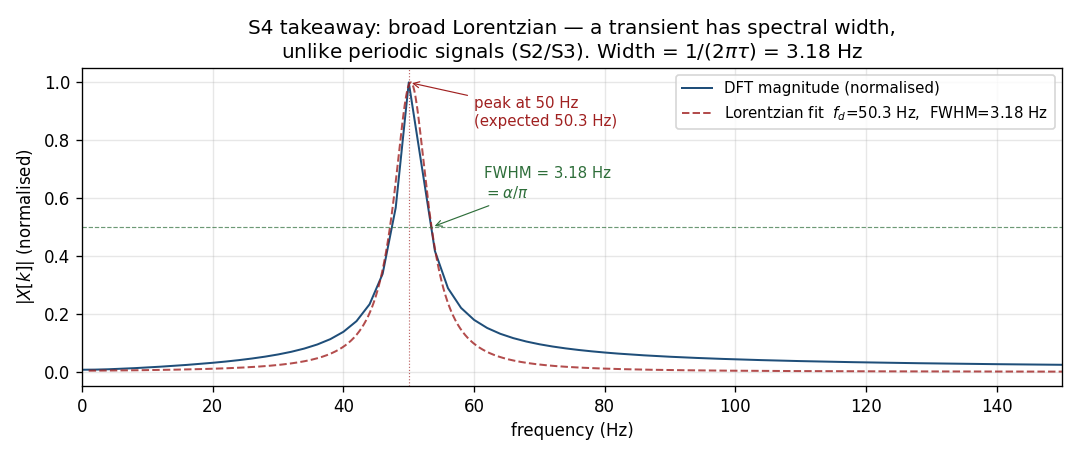
\includegraphics[width=0.92\textwidth]{figures/fig-b1-s4-takeaway.png}}{%
  \fbox{\parbox{0.82\textwidth}{\centering\itshape fig-b1-s4-takeaway.png}}}
\end{center}
\end{pipelinestep}

\paragraph{What S4 shows.}
A smooth Lorentzian centred at $f_d \approx 50\,\mathrm{Hz}$.
The half-power width (FWHM) is $\alpha/\pi = 3.18\,\mathrm{Hz}$
--- directly readable from the spectrum as the inverse of the
decay time constant: $\tau = 1/\alpha = \pi/\mathrm{FWHM} \approx
100\,\mathrm{ms}$. A long-lived oscillation (small $\alpha$) has a
narrow spectrum; a quickly-damped transient has a wide spectrum.
This is the time-frequency uncertainty principle, presented here
without ceremony as a thing that simply falls out of the arithmetic.
A resistor, asked directly, is more honest about Heisenberg than most
physicists.

\section{Cross-fixture synthesis}

\begin{longtable}{p{1.5cm}p{3.5cm}p{4.0cm}p{4.5cm}}
\toprule
\textbf{Signal} & \textbf{Time domain} & \textbf{Frequency domain} & \textbf{What the DFT measures} \\
\midrule
\endhead
S1 muon & Exponential decay + background floor & Broad Lorentzian + flat floor; no periodic structure & Decay time scale; background level \\
S2 square & Sharp periodic transitions & Sparse odd harmonics, $1/n$ envelope & Harmonic content of a one-period shape \\
S3 triangle & Smooth periodic ramps & Same odd harmonics, $1/n^2$ envelope & Shape difference encoded in amplitude falloff \\
S4 RLC & Decaying oscillation & Smooth Lorentzian; FWHM $= 1/(2\pi\tau)$ & Resonance frequency and damping \\
\bottomrule
\end{longtable}

The DFT does not know about physics. It measures \emph{which
sinusoidal components are present and at what amplitude}. It is, in
this sense, the most aggressively agnostic instrument in the
toolbox: it will give you the same kind of answer whether you feed
it the decay curve of a subatomic particle, the output of a function
generator, or the ringing of an electrical circuit. Physics happens
to all four of these signals; the DFT does not care which physics
and produces, in every case, a spectrum.

The four cases are the four canonical scenarios: pure pulse or
transient (S1, S4), pure harmonic series (S2), tapered harmonic
series (S3). Everything a scope can show falls into one of these
families or a mixture of them. By the time you reach the end of B5
you will recognise these four shapes in radar returns, audio
recordings, machine-vibration data, and the output of an electronic
filter chain. The signals will look very different. The spectra will
look like cousins of these four.

\section{Try it yourself}

\begin{lstlisting}[style=shaddata]
$ cd examples/shad/b1-scope

# S1: fetch once (~1 MB)
$ python probe_b1_muon.py

# S2, S3, S4: instantaneous (no download)
$ python probe_b1_squarewave.py
$ python probe_b1_triangle.py
$ python probe_b1_rlc.py

# Render all 12 figures
$ python render_b1_s1.py
$ python render_b1_s2.py
$ python render_b1_s3.py
$ python render_b1_s4.py
\end{lstlisting}

\textbf{S1 licence note.} The Rodriguez muon dataset is not redistributed
with this repository. \texttt{probe\_b1\_muon.py} fetches it from
\url{amor.cms.hu-berlin.de/~rodrigus}. Public reproduction requires
written permission from Santiago Rodriguez with full attribution
\cite{Rodriguez2018}.



% ======================================================================
% B2 — Audio: polyphony, leakage, windowing
% ======================================================================
\chapter{B2 --- audio: polyphony, leakage, windowing}
\label{ch:b2}

\section{The premise}

The ear contains, in its innermost chamber, a structure called the basilar
membrane --- a roughly 35-millimetre spiral that is narrow and stiff at one
end, wide and floppy at the other. Different frequencies cause different parts
of it to resonate: high frequencies near the stiff end; low frequencies at the
floppy end. The result is a spatial frequency map, read out along the spiral
and reported, already decomposed, to the brain. The ear has been running this
particular computation for approximately 50 million years, which is a
considerable head start on the laboratory
equipment.\footnote{The outer ear canal, eardrum, and three small bones
upstream of the cochlea are the preprocessing chain; the basilar membrane does
the frequency-sorting. The analogy to a DFT is imperfect but instructive ---
and the human version comes with a carry case and does not require a power
supply.}

A chord is several of those frequencies arriving simultaneously, each staking
a claim on a different portion of the membrane. The DFT is how we confirm ---
computationally, without the biology --- which frequencies are present and at
what relative strength. This chapter applies the same four-step pipeline as
B1, but against a piece of audio with three notes in it. The spectrum will
have three peaks. One of them, as it happens, will not land exactly where it
should, and that small displacement will turn out to be rather informative.

This chapter does two things B1 didn't:
\begin{enumerate}[label=\arabic*.,leftmargin=*,itemsep=0pt]
\item Multiple peaks at once.
\item \textbf{Spectral leakage}, and how a window function tames it.
\end{enumerate}

\section{The input}

\texttt{examples/shad/b2-audio/main.py} synthesises a C-major triad:
C4 (261.63\,Hz) + E4 (329.63\,Hz) + G4 (392.00\,Hz), summed at relative
amplitudes 0.4, 0.3, 0.3, sampled at 44.1\,kHz (CD quality) for 500\,ms.

\begin{center}
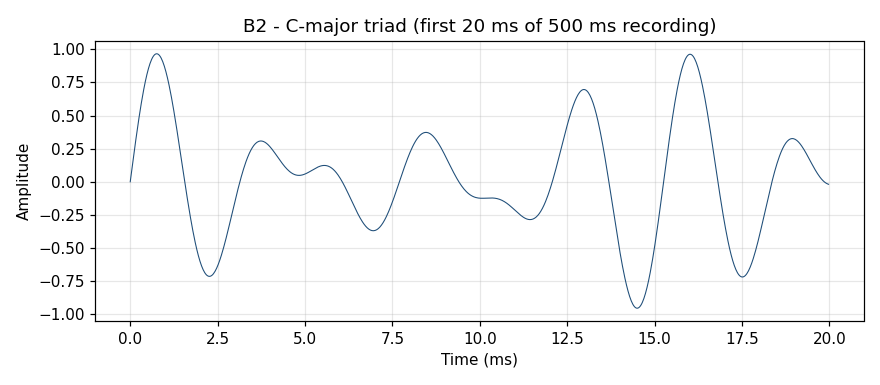
\includegraphics[width=0.92\textwidth]{figures/fig-b2-input}
\end{center}
\textit{Twenty milliseconds of waveform shown --- the full 500\,ms would look
like a solid black band. The pattern visible is the \textbf{beat} between the
three notes: their frequencies aren't simple integer ratios, so the combined
waveform doesn't perfectly repeat at a short interval.}

To the eye, the waveform looks like elegant chaos. It is three sinusoids,
patiently coexisting --- what the ear decodes automatically in milliseconds,
the DFT will decode in microseconds, at the cost of four lines of Python.

\section{The transform --- first pass, rectangular window}

Same code as B1, except $N$ is bigger: 22\,050 samples instead of 500.

\begin{pipelinestep}{Step 3. Transform --- rectangular window (no windowing)}
\begin{lstlisting}[style=shadpython]
n = samples.size                          # 22050
spec = np.fft.fft(samples) / n
freq = np.fft.fftfreq(n, d=1.0/44_100)
half = n // 2
freq, mag = freq[:half], np.abs(spec[:half])
\end{lstlisting}
\end{pipelinestep}

\begin{center}
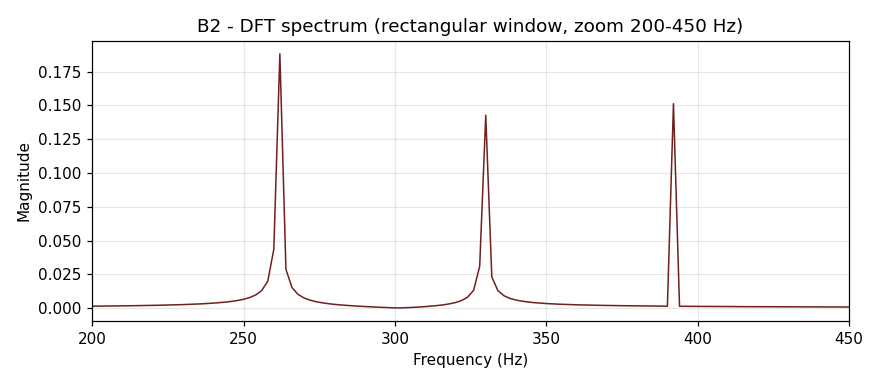
\includegraphics[width=0.92\textwidth]{figures/fig-b2-spectrum}
\end{center}
\textit{B2 spectrum, rectangular window. Zoomed to 200--450\,Hz. Three peaks.
The C4 peak at 261.63\,Hz shows visible side-lobes; G4 at 392.00\,Hz lands
cleanly on a bin; C4 and E4 do not.}

Three peaks. Good. But look closely at the C4 peak at 261.63\,Hz: it has
visible \textbf{side-lobes} spreading energy into neighbouring bins. The G4
at 392\,Hz lands right on a bin (392.00\,Hz $\times$ 22050 $\div$ 44100
$= 196.0$, exact integer) and looks clean. The C4 and E4 don't land on
integer bins, so their energy spreads.

This is \textbf{spectral leakage}. \textbf{Do not panic about this.} The name
sounds as though something went wrong; nothing went wrong. What happened is
that the DFT implicitly treats your 500\,ms recording as one period of an
infinitely-repeating signal --- and if a frequency doesn't divide evenly into
the recording length, the DFT sees a discontinuity at the boundaries, and that
discontinuity smears energy into neighbouring bins. The signal is still there.
The three notes are still identifiable. The leakage is the DFT being honest
about the mismatch between the signal and its window --- which is, as forms of
honesty go, more diagnostic than most instruments manage.

\section{Windowing}

The fix: multiply the input by a window function before transforming. The
window tapers the signal smoothly to zero at both ends, which reduces the
artefacts caused by the DFT implicitly treating your 500\,ms recording as one
period of an infinitely-repeating signal.

\begin{pipelinestep}{Step 3b. Transform --- Hann window applied}
\begin{lstlisting}[style=shadpython]
n = samples.size
w = np.hanning(n)               # Hann window: 0 at ends, 1 in middle
x = samples * w
gain = w.sum() / n              # coherent gain compensation
spec = np.fft.fft(x) / (n * gain)
\end{lstlisting}
\end{pipelinestep}

The \texttt{gain} factor compensates for the energy the window removed at
the edges, so the peak heights still match the original tone amplitudes.
The Hann window\footnote{Named for Julius von Hann, a 19th-century Austrian
meteorologist who studied atmospheric pressure oscillations. The colloquial
spelling ``Hanning'' is factually inexact but universally understood. Julius
himself has no recorded opinion on the matter.} tapers with a raised cosine
--- smooth enough to suppress most leakage without broadening the main peaks
too badly.

\section{The takeaway}

\begin{center}
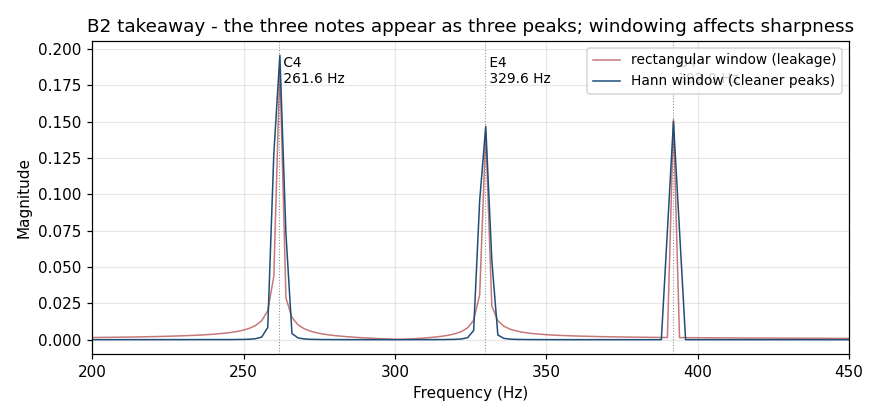
\includegraphics[width=0.92\textwidth]{figures/fig-b2-takeaway}
\end{center}
\textit{Two spectra overlaid: red = rectangular window (side-lobes visible
around each peak); blue = Hann window (peaks slightly wider but inter-peak
noise drops dramatically). Rendered by
\texttt{examples/shad/b2-audio/main.py}.}

Which window to use is a domain-dependent choice. Hann is the
default-good-choice for general analysis; Hamming is similar; Blackman gives
narrower side-lobes at the cost of a slightly wider main-lobe; rectangular is
fine when your frequencies land exactly on integer bins (rare in real signals).

This is, in miniature, the central trade-off of spectral analysis: narrow peaks
or low side-lobes --- not both simultaneously. Every window function is a
negotiation between these two quantities. The choice is a judgment call, not a
theorem, which is either reassuring or alarming depending on your disposition
toward ambiguity.

\section{What we just did}

\textbf{Multiple peaks, with leakage.} This is what real-world spectra look
like 95\% of the time. The takeaway plot is what a music-analysis tool would
show you for any chord. The same machinery applies to:
\begin{itemize}[leftmargin=*,itemsep=0pt]
\item Speech analysis (which formant frequencies are present in a vowel)
\item Vibration monitoring (which rotation-rate harmonics show up --- that
  is Chapter~\ref{ch:b3})
\item Radar / sonar (which Doppler-shifted reflectors are in your sight line)
\item Any spectrum analyser hardware you have ever looked at
\item Any signal sampled at regular intervals in time --- which, depending on
  how broadly you read the word ``signal'', is most of the numerical data that
  has ever been collected
\end{itemize}

\section{Try it yourself}

\begin{lstlisting}[style=shaddata]
python examples/shad/b2-audio/main.py
\end{lstlisting}

Modify the \texttt{NOTE\_FREQ} dictionary at the top of \texttt{main.py} to
play different chords. Try minor triads (C4 + E$\flat$4 + G4 = 261.63 +
311.13 + 392.00\,Hz). Try dissonances (C4 + C$\sharp$4). Note how the
spectrum reads exactly what you would hear. For real audio: the script's
bottom has a sketch showing how to drop in any CC-licensed \texttt{.wav}
from Wikimedia Commons or Freesound. The transform code is identical; only
the data source changes.

% ======================================================================
% B3 — Vibration: harmonics and fault signatures
% ======================================================================
\chapter{B3 --- vibration: harmonics and fault signatures}
\label{ch:b3}

\section{The premise}

There is a particular skill, practiced by experienced maintenance engineers on
factory floors, of listening to a machine and knowing whether something is
wrong.\footnote{The limitation being that two ears, one brain, and ambient
factory noise are not a calibrated measurement system. The engineers are not
wrong that they can hear something; they are sometimes wrong about what it is.}
They walk the floor with nothing but a screwdriver, press the handle against a
motor casing, put an ear to the blade end, and diagnose by sound. The 1$\times$
shaft tone feels like a hum; an imbalance adds a subtler oscillation; a worn
bearing has a characteristic tick at a frequency that varies with rotational
speed. This sounds like superstition --- and in the hands of an inexperienced
listener, it is. In the hands of somebody who has spent five years doing it,
it is surprisingly reliable.

It is also not scalable. What you can have instead is an accelerometer, a data
logger, a DFT, and the knowledge of what to look for in the resulting
\textbf{vibration spectrum}. The maths does the listening at scale, and the
spectrum does what the screwdriver-and-ear method always wanted to do but
couldn't quite manage: quantify.

B1 had a clean tone. B2 had a chord. \textbf{Real industrial machines don't
produce clean tones.} A rotating bearing produces a fundamental shaft rate
plus integer-multiple harmonics (imbalance, misalignment, looseness) plus
non-integer features (bearing-fault signatures, gearmesh sidebands) plus a
broadband noise floor. A trained vibration engineer reads these spectra the
way a doctor reads an ECG. This chapter shows you the basics.

\section{The setup}

\texttt{examples/shad/b3-vibration/main.py} synthesises a 2-second
accelerometer trace from a machine running at 1800\,RPM (= 30\,Hz shaft
rate), sampled at 5\,kHz. The synthetic signal contains:

\medskip
\begin{longtable}{p{2.8cm}p{2.2cm}p{1.8cm}p{7.2cm}}
\toprule
\textbf{Feature} & \textbf{Frequency} & \textbf{Amplitude}
  & \textbf{Physical meaning} \\
\midrule
\endhead
\textbf{1$\times$ (shaft)} & 30.0\,Hz & 1.00
  & The fundamental rotation rate \\
\textbf{2$\times$ (imbalance)} & 60.0\,Hz & 0.40
  & Mass imbalance on the rotor \\
\textbf{3$\times$ (alignment)} & 90.0\,Hz & 0.25
  & Coupling misalignment between shafts \\
\textbf{BPFO (fault)} & 142.4\,Hz & 0.30
  & Ball-pass frequency, outer race --- incipient bearing fault \\
\bottomrule
\end{longtable}
\medskip

Plus a white-noise floor at 5\% amplitude.

The first three are \emph{harmonics} of the shaft rate --- integer multiples
of 30\,Hz, predictable from the shaft speed alone. The BPFO at 142.4\,Hz is
a different matter entirely. \textbf{Do not panic if the number looks strange.}
The BPFO is \textbf{not} an integer multiple of 30\,Hz --- it is determined by
the bearing geometry (number of balls, ball diameter, pitch diameter, contact
angle).\footnote{Every bearing has a published BPFO --- the manufacturer
provides it, or you calculate it from the geometry using a formula that has
been in the engineering literature since the 1960s. If the spectrum shows a
peak at exactly that frequency, the outer race is damaged. If it doesn't:
either the bearing is healthy, or you need better windowing to surface the
peak from the noise floor.}
On this bearing, the calculated BPFO is $4.746\times$ shaft rate, giving
142.4\,Hz at 30\,Hz shaft. The non-integer comes from the geometry of the
balls rolling against the outer race, not from any fault in the maths.

\section{The input}

\begin{center}
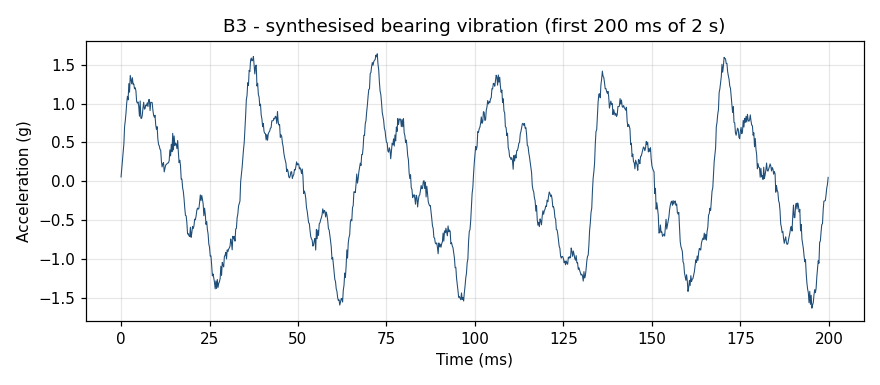
\includegraphics[width=0.92\textwidth]{figures/fig-b3-input}
\end{center}
\textit{First 200\,ms shown. The dominant 30\,Hz rotation is visible visually
(about 6 full cycles in 200\,ms). The smaller-amplitude features blend into
a complex waveform.}

\section{The transform --- Hann-windowed}

For real-world vibration data, you essentially \emph{always} window. The data
isn't periodic over your record length, so a rectangular window gives leakage
that obscures the BPFO peak.

\begin{pipelinestep}{Step 3. Transform --- Hann-windowed vibration spectrum}
\begin{lstlisting}[style=shadpython]
n = samples.size                            # 10000 (5 kHz x 2 s)
w = np.hanning(n)
spec = np.fft.fft(samples * w) / (n * w.sum() / n)
freq = np.fft.fftfreq(n, d=1.0/5_000)
half = n // 2
freq, mag = freq[:half], np.abs(spec[:half])
\end{lstlisting}
\end{pipelinestep}

\begin{center}
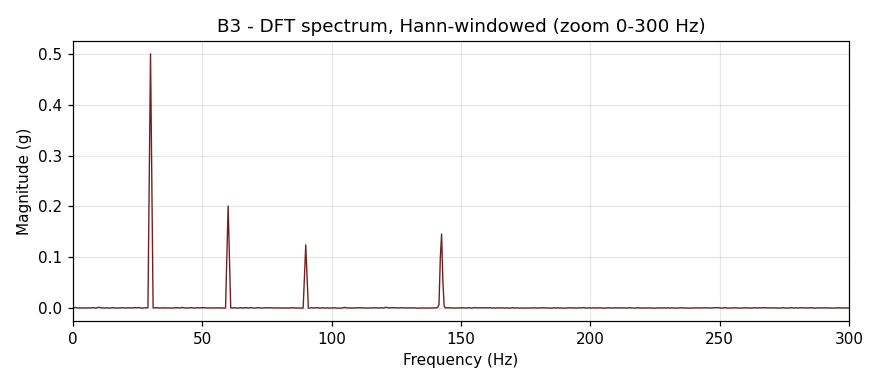
\includegraphics[width=0.92\textwidth]{figures/fig-b3-spectrum}
\end{center}
\textit{B3 spectrum, Hann-windowed. Four distinct features visible in the
0--300\,Hz range.}

\section{The takeaway --- what a vibration engineer sees}

\begin{center}
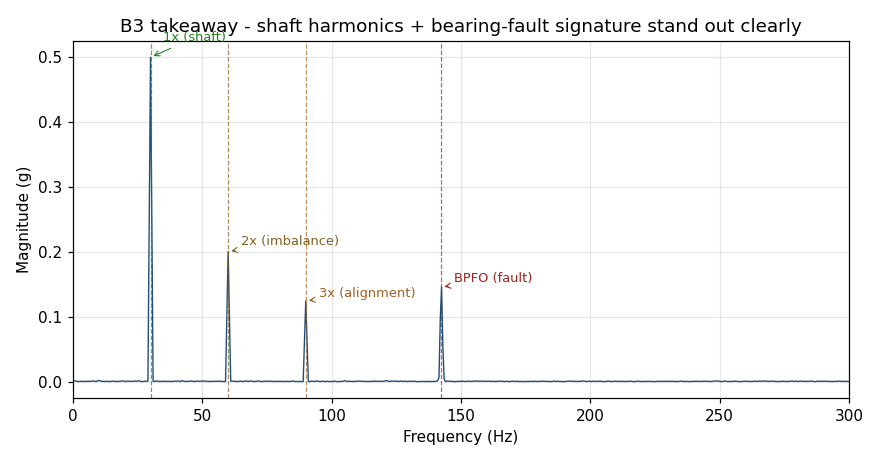
\includegraphics[width=0.92\textwidth]{figures/fig-b3-takeaway}
\end{center}
\textit{Annotated spectrum. \textbf{Diagnostic reading}, working through what
the four peaks tell you:
(1) 30\,Hz (1$\times$) dominant: shaft is rotating, sensor working.
(2) 60\,Hz (2$\times$) at 0.40$\times$: moderate imbalance.
(3) 90\,Hz (3$\times$) at 0.25$\times$: mild alignment issue.
(4) 142.4\,Hz (BPFO) at 0.30$\times$: incipient outer-race bearing damage.}

This is the kind of analysis that turns spectrum plots into maintenance
schedules. Every condition-monitoring system on the planet (SKF, Bently
Nevada, GE/Bently, IFM, OEM custom solutions) is essentially doing what
we just did: take samples, window, FFT, look up peaks against expected fault
frequencies, report.

\section{What we just did}

\textbf{Spectrum as diagnostic.} The spectral pattern carries more information
than the time-domain trace because \emph{each rotating-machinery failure mode
has its own signature frequency}. Misalignment is always at integer harmonics.
Bearing faults are always at one of the four ball-related frequencies (BPFO,
BPFI, BSF, FTF). Gearmesh defects are always at the gearmesh frequency. Once
you know the catalogue, the spectrum reads itself.

Vibration analysis is the most mature ``spectrum is the answer'' engineering
domain --- it has been the standard for predictive maintenance since the
1970s.\footnote{Cooley and Tukey published the FFT in 1965. By the 1970s, it
had migrated from university mainframes to dedicated portable analysers small
enough to carry onto a factory floor. An algorithm that went from a four-page
journal paper to a ubiquitous industrial instrument in under a decade is, by
historical standards, moving rather fast.}
The maths you just learned in B1 and B2 is the \emph{entirety} of the maths
behind a multi-billion-dollar industry's bread-and-butter analysis tool.

\section{Try it yourself}

\begin{lstlisting}[style=shaddata]
python examples/shad/b3-vibration/main.py
\end{lstlisting}

Modify the \texttt{HARMONICS} dict at the top of \texttt{main.py} to simulate
different fault scenarios:
\begin{itemize}[leftmargin=*,itemsep=0pt]
\item Crank up \texttt{2x (imbalance)} to 1.5 $\rightarrow$ severe imbalance,
  dominant peak shifts from 1$\times$ to 2$\times$.
\item Add a new entry \texttt{"BPFI (inner race)": (235.2, 0.4)} $\rightarrow$
  a different bearing fault.
\item Reduce \texttt{1x (shaft)} to 0.3 and set \texttt{noise\_amp} to 0.2
  $\rightarrow$ a noisy machine with a small but persistent BPFO peak: the
  analyst's nightmare scenario where you need careful windowing to detect the
  fault buried in noise.
\end{itemize}

% ======================================================================
% B4 — Electronic systems: filters, mixers, oscillators
% ======================================================================
\chapter{B4 --- electronic systems: filters, mixers, oscillators}
\label{ch:b4}

\section{The premise}

The word ``filter'' is borrowed from coffee, from water treatment, from air
conditioning --- and in each context it means approximately the same thing:
a structure that lets some things through and stops the rest. The filter has
no editorial preferences. It has a physical structure, and that structure
determines what passes.

Electronic versions of the same idea work on exactly this principle, except
that the things being sorted are not particles or molecules but frequency
components --- sinusoidal elements that coexist inside a complicated waveform
and can, rather surprisingly, be extracted from it individually. That this
extraction is possible at all was not obvious to anyone before approximately
1807, when a French administrator and mathematical physicist named Joseph
Fourier argued that any periodic function could be decomposed into sines and
cosines. He was told his proof had a gap in it.\footnote{The 1807 paper was
submitted to the Institut de France and reviewed by Lagrange, Laplace, and
Monge, who found the convergence argument incomplete. Fourier continued doing
it anyway. The 1822 \emph{Th\'{e}orie analytique de la chaleur} was the
version that properly established the result; Dirichlet filled in the last
piece in 1829. The man responsible for ``any signal can be decomposed into
frequencies'' had to wait twenty-two years for full mathematical vindication
--- which is, in retrospect, not how you'd choose to run things.}

B3 showed you a spectrum you could only \emph{observe}. The machine was
already spinning; the fault was already there. Fourier handed you a picture.

\textbf{B4 is different.} In electronics, you actively \emph{design} for
frequency-domain behaviour. A filter is literally defined by which frequencies
it passes and which it kills. A radio receiver is deliberately moving
frequencies around. The spectrum view is not a diagnostic aid here --- it is
the primary engineering language.

Three sub-topics, each adding one layer to the same idea: active circuits
change the spectrum, and you can predict exactly how.

\section{1. AC mains harmonics --- what is actually in that socket?}

\subsection{The setup}

You probably learned that mains is a ``50\,Hz sine wave.'' It is not.
Everything you plug in that contains a rectifier (phone charger, computer
power supply, LED dimmer) draws current in narrow pulses rather than
sinusoidally. That non-linear current draw distorts the mains voltage,
injecting energy at odd harmonics of the 50\,Hz fundamental.

\texttt{examples/shad/b4-electronic/main.py} synthesises a realistic mains
waveform:

\medskip
\begin{longtable}{p{3.5cm}p{2.2cm}p{3.0cm}p{4.8cm}}
\toprule
\textbf{Harmonic} & \textbf{Frequency} & \textbf{Rel.\ amplitude}
  & \textbf{Source} \\
\midrule
\endhead
\textbf{1st (fundamental)} & 50\,Hz & 1.000 & The line itself \\
\textbf{3rd} & 150\,Hz & 0.040 & Single-phase rectifiers \\
\textbf{5th} & 250\,Hz & 0.025 & Switching power supplies \\
\textbf{7th} & 350\,Hz & 0.015 & Accumulated load mix \\
\textbf{9th} & 450\,Hz & 0.008 & Distributed building load \\
\bottomrule
\end{longtable}
\medskip

Total Harmonic Distortion: \textbf{THD = 5.0\%} --- typical residential grid.

\subsection{The input and spectrum}

\begin{center}
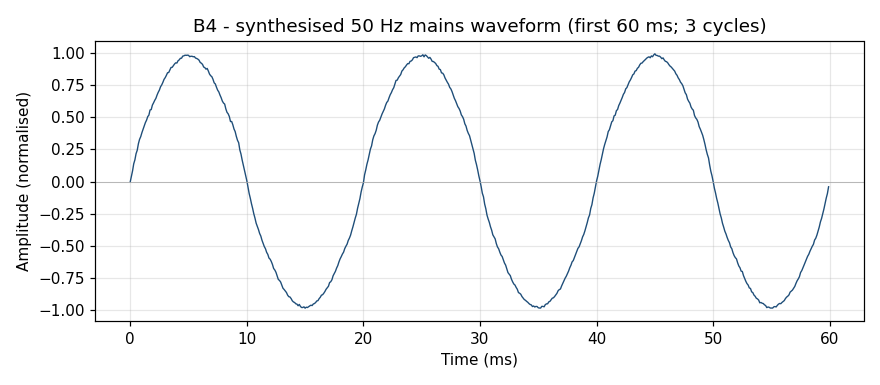
\includegraphics[width=0.92\textwidth]{figures/fig-b4-input}
\end{center}
\textit{Three cycles of 50\,Hz mains. The distortion from harmonics is visible
as a slight flattening near each peak. This is the signal arriving at your
equipment's input terminals every day.}

\begin{center}
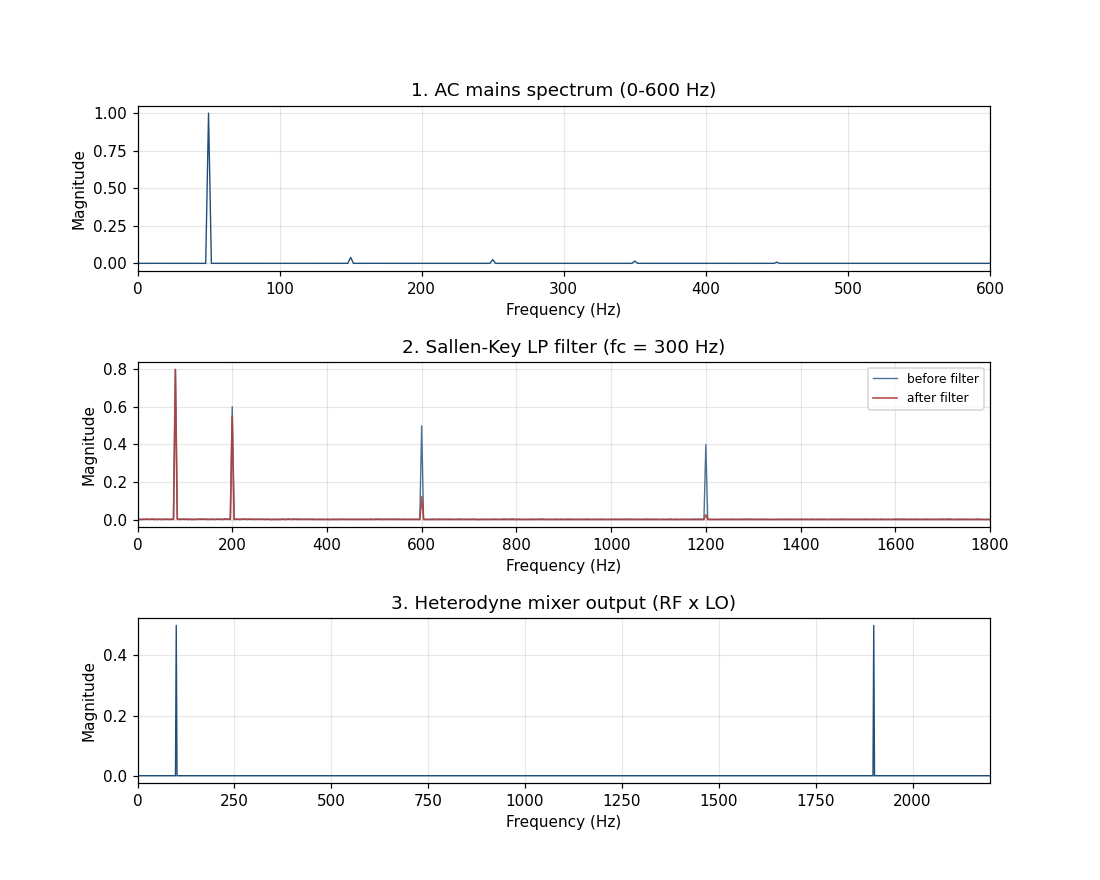
\includegraphics[width=0.92\textwidth]{figures/fig-b4-spectrum}
\end{center}
\textit{Top panel: mains spectrum, 0--600\,Hz. Five peaks. Fundamental at
50\,Hz dominates; odd harmonics fall off to the right. Middle panel: test
signal before and after the Sallen-Key filter (300\,Hz cutoff). Bottom panel:
mixer output spectrum, 0--2200\,Hz.}

\subsection{The takeaway --- reading the mains spectrum}

\begin{center}
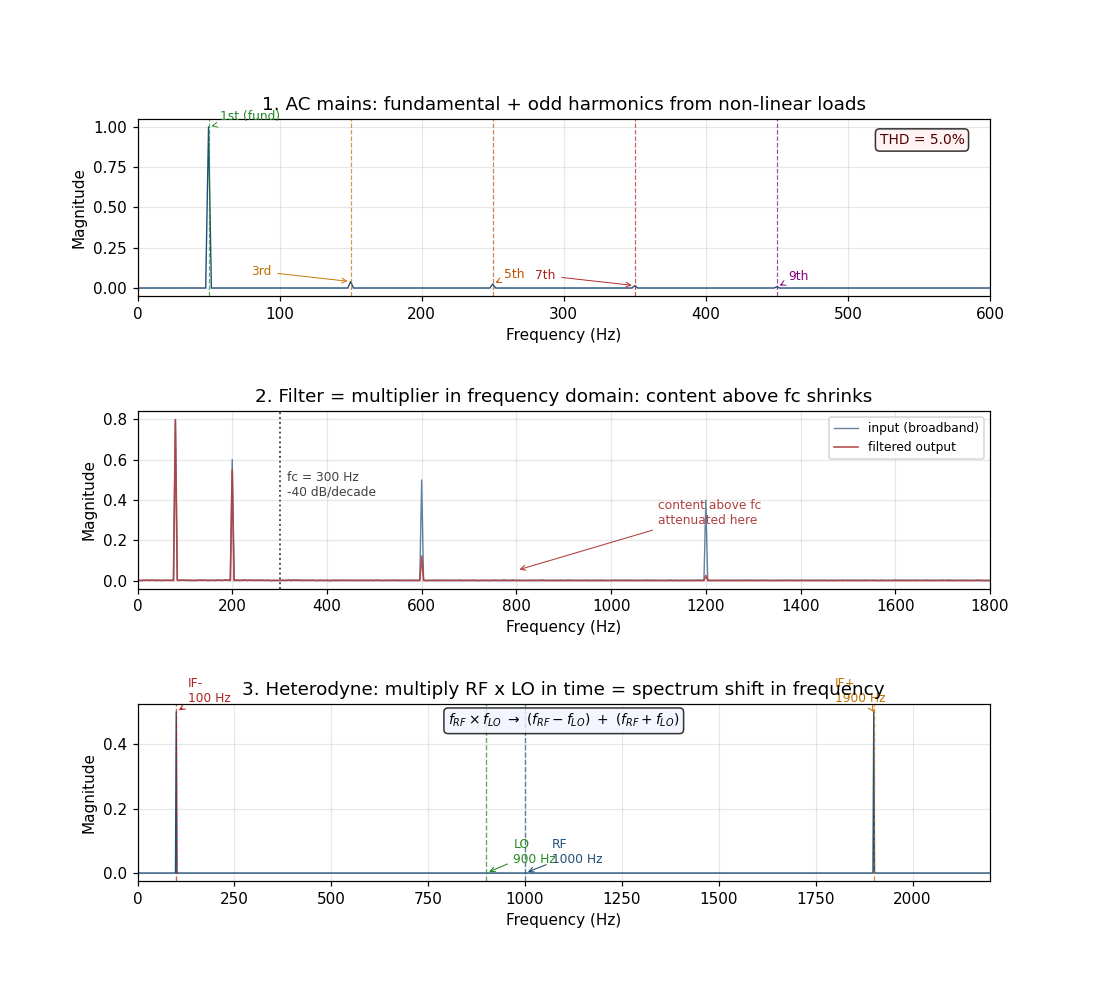
\includegraphics[width=0.92\textwidth]{figures/fig-b4-takeaway}
\end{center}

The standard metric is \textbf{THD} (Total Harmonic Distortion):
\begin{lstlisting}[style=shaddata]
THD = sqrt(V_3^2 + V_5^2 + V_7^2 + V_9^2 + ...) / V_1
\end{lstlisting}

IEEE\,519-2022 sets acceptable THD limits: typically $<5\%$ THD-V at the point
of common coupling for most industrial systems. A THD above these thresholds
has measurable consequences: motor heating (harmonics produce heat, not useful
torque), transformer derating (K-factor 0.85--0.95 for moderately distorted
supply), and EMC pre-compliance (IEC\,61000-3-2 limits are an FFT of input
current, checked against a published table --- that compliance test \emph{is}
what we just computed).

\section{2. Active filter --- filtering IS multiplication in frequency}

\subsection{The setup}

The goal: suppress the 5th, 7th, and 9th mains harmonics from a sensitive
analogue measurement circuit. You install a 2nd-order Sallen-Key low-pass
filter with a cutoff at 300\,Hz.\footnote{R.\,P. Sallen and E.\,L. Key
published this active-filter topology in a 1955 paper while working at MIT
Lincoln Laboratory. Its practical virtue was that it achieved a 2nd-order
response with no inductors --- audio-frequency inductors are large, expensive,
and have a tendency to pick up interference from nearby transformers.}

The Sallen-Key transfer function (normalised LP):
\begin{lstlisting}[style=shaddata]
H(f) = 1 / (1 + j*(f/fc)/Q - (f/fc)^2)
\end{lstlisting}

\textbf{Do not panic about the \texttt{j} in that expression.} The \texttt{j}
is the imaginary unit ($\sqrt{-1}$), doing one specific job: encoding the
phase shift the filter introduces at each frequency --- a real physical effect.
The modulus $|H(f)|$ comes out to a real positive number, and that is the only
number you need to read a plot.

For a Butterworth (maximally flat) response: $Q = 1/\sqrt{2} = 0.707$. Above
the cutoff the response rolls off at $-40$\,dB/decade.

The script applies this filter entirely in the frequency domain: compute the
FFT of the input, multiply by $H(f)$, inverse-FFT back to time. This is not a
trick --- it is exactly what the physical capacitors and op-amp are doing, just
described in different notation.

\section{3. Heterodyne mixer --- shifting the spectrum}

\subsection{The setup}

A superheterodyne receiver wants to shift an incoming RF signal at an
arbitrary frequency down to a fixed intermediate frequency (IF) where it can
be filtered and amplified efficiently.

In 1918, Edwin Howard Armstrong\footnote{Armstrong's superheterodyne patent
was contested by Lee de Forest and later by RCA for years. Armstrong won the
legal arguments but spent most of his fortune doing so, and did not live to see
the principle become the architectural basis of every radio receiver manufactured
for the rest of the twentieth century. He died in 1954.}
demonstrated that you could shift any incoming signal to a single fixed
intermediate frequency by multiplying it against a tunable local oscillator.

The mechanism: \textbf{multiply the RF signal by a local oscillator (LO) in
the time domain.} Trigonometric identity:
\begin{lstlisting}[style=shaddata]
sin(2*pi*f_RF*t) * sin(2*pi*f_LO*t)
    = 0.5 * [cos(2*pi*(f_RF - f_LO)*t) - cos(2*pi*(f_RF + f_LO)*t)]
\end{lstlisting}

The product produces two new frequencies: the \textbf{difference} (RF $-$ LO)
and the \textbf{sum} (RF $+$ LO). In a receiver, you choose LO so that the
difference falls at a convenient IF; you then filter out the sum.

The script uses: RF = 1000\,Hz, LO = 900\,Hz, IF$^- =$ RF $-$ LO = \textbf{100\,Hz}
(desired output), IF$^+ =$ RF $+$ LO = \textbf{1900\,Hz} (image, filtered out).

Why does this matter beyond radios? The same heterodyne principle appears in
lock-in amplifiers, optical coherence tomography, software-defined radio, and
gravitational-wave detectors --- LIGO uses optical heterodyne interferometry
to detect mirror displacements smaller than one-thousandth of a proton
diameter.

\section{What we just did}

Three sub-topics, one unifying claim: \textbf{the spectrum is the primary
design language for active circuits.} An oscilloscope shows you what happened.
A spectrum analyser shows you what will happen if you add a filter, swap a
component, or mix in an oscillator. The difference between B3 (observation)
and B4 (design) is the difference between diagnosis and engineering. The
spectrum doesn't care which one you're doing. It reports the frequencies. It
has always reported the frequencies.

% ======================================================================
% B5 — Radar: Doppler, range-Doppler, pulse compression
% ======================================================================
\chapter{B5 --- radar: Doppler, range--Doppler, pulse compression}
\label{ch:b5}

\section{The premise}

Christian H\"{u}lsmeyer was a German engineer with a sensible idea and
unfortunate timing. In 1904, he demonstrated a device he called the
Telemobiloskop --- a radio transmitter and receiver arranged to detect ships
in fog by listening for the echoes off their hulls. The Imperial German Navy
inspected the demonstration, concluded that they already had binoculars, and
declined to purchase.\footnote{The British reinvention --- Chain Home,
operational by 1937 --- formed part of an integrated air-defence system whose
contribution to the Battle of Britain is difficult to overstate.
H\"{u}lsmeyer is celebrated as the inventor of radar in the footnotes of the
history books. The footnotes of the history books are not a comfortable place
to be celebrated.}

What H\"{u}lsmeyer had demonstrated is that radio echoes carry quantitative
information. Not merely ``something is there'' information, but \emph{where}
it is and \emph{how fast} it is moving, both derivable from the timing and
frequency of the returning signal. Extracting those quantities cleanly turns
out to be the problem the Fourier transform was built to solve.

B4 showed you circuits that multiply in the frequency domain. \textbf{B5 is
the same idea, taken to its natural extreme.} A radar transmits a
precisely-crafted waveform, listens for the echo, and uses the Fourier
machinery to answer two questions: \emph{where is it} and \emph{how fast is
it going}. Everything that follows is three Fourier operations stacked in
sequence. The same \texttt{np.fft.fft} you used to look at a 50\,Hz mains
waveform is doing the work.

\section{1. The pulse --- what you transmit}

A plain rectangular pulse has a resolution problem: short pulses carry little
energy, limiting range. The solution: \textbf{transmit a long pulse with a
frequency sweep --- a chirp.}

The transmit waveform is a linear-FM chirp:
\begin{lstlisting}[style=shaddata]
s_tx(t) = exp(j * pi * K * t^2),   0 <= t < tau
\end{lstlisting}

where $K = \mathrm{BW}/\tau$ is the chirp rate (Hz/s). \textbf{Do not panic
about the \texttt{j} in the exponent.} It means the chirp is represented as a
complex-valued signal --- a bookkeeping convention that keeps the phase
arithmetic clean through the three Fourier stages that follow.

\medskip
\begin{longtable}{p{3.0cm}p{2.0cm}p{8.0cm}}
\toprule
\textbf{Parameter} & \textbf{Value} & \textbf{Physical meaning} \\
\midrule
\endhead
Carrier $f_c$ & 2.8\,GHz & S-band (weather radar) \\
Pulse duration $\tau$ & 1.6\,$\mu$s & Long pulse = energy \\
Chirp BW & 0.625\,MHz & Determines range resolution \\
Chirp rate $K$ & $3.9 \times 10^{11}$\,Hz/s & $= \mathrm{BW}/\tau$ \\
Sample rate $f_s$ & 2\,MHz & $= 2 \times \mathrm{BW}$ (Nyquist) \\
\bottomrule
\end{longtable}
\medskip

Range resolution from the bandwidth: $\delta R = c / (2 \cdot \mathrm{BW})
= \mathbf{240\,m}$. You cannot distinguish two targets closer than 240\,m
in range.

\begin{center}
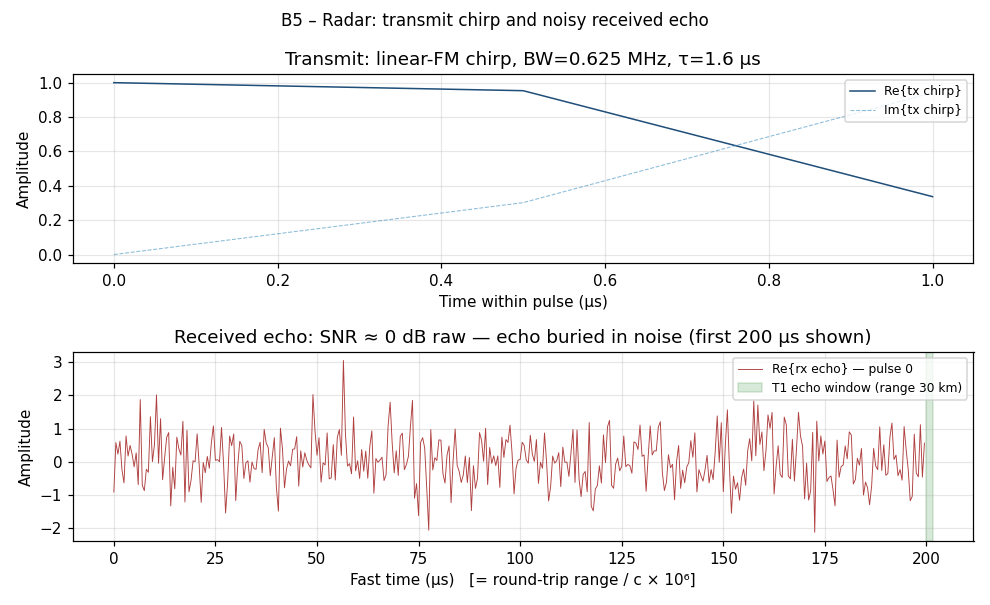
\includegraphics[width=0.92\textwidth]{figures/fig-b5-input}
\end{center}
\textit{Top: transmit chirp (real part shows frequency sweep). Bottom: received
echo from first 200\,$\mu$s --- the target is invisible at SNR $= 0$\,dB before
processing. Three targets were synthesised: T1 (30\,km, +20\,m/s), T2
(65\,km, 0\,m/s), T3 (110\,km, $-35$\,m/s).}

\section{2. Matched-filter pulse compression}

You know exactly what you transmitted. The echo is a delayed, attenuated,
Doppler-shifted copy, buried in noise. The optimal strategy is the
\textbf{matched filter}: correlate the received signal with the known transmit
waveform. In frequency domain, convolution is multiplication:

\begin{pipelinestep}{Stage 1+2. Matched-filter pulse compression}
\begin{lstlisting}[style=shadpython]
def matched_filter_compress(raw_matrix, chirp):
    N_FFT   = N_RANGE
    chirp_padded = np.zeros(N_FFT, dtype=np.complex128)
    chirp_padded[:N_SAMP_PU] = chirp
    TX      = np.fft.fft(chirp_padded)   # transmit reference spectrum
    TX_CONJ = np.conj(TX)                # conjugate = matched filter kernel
    compressed = np.zeros_like(raw_matrix)
    for p in range(N_PULSES):
        RX = np.fft.fft(raw_matrix[:, p], n=N_FFT)
        compressed[:, p] = np.fft.ifft(RX * TX_CONJ).real
    return compressed
\end{lstlisting}
\end{pipelinestep}

That is it. \texttt{compressed(t) = IFFT(FFT(rx) $\times$ conj(FFT(tx)))}.
The Fourier operation you have been using to look at spectra is now being
used to extract a target from noise 20\,dB below the floor.

\textbf{Processing gain:}
\begin{lstlisting}[style=shaddata]
SNR_out = SNR_in + 10*log10(BW * tau) + 10*log10(N_pulses)
        ~= 0 dB + 0 dB + 18 dB = 18 dB
\end{lstlisting}

The 18\,dB comes from coherently integrating 64 pulses.

\section{3. Doppler --- the second Fourier operation}

After pulse compression you have a matrix \texttt{compressed[range\_bin, pulse\_index]}.
A target at fixed range appears in the same range bin across all 64 pulses ---
but its phase shifts between pulses by $\Delta\phi = 2\pi \cdot f_d / \mathrm{PRF}$,
where $f_d = 2 v_r f_c / c$ is the Doppler frequency.\footnote{Named for
Christian Doppler, an Austrian physicist who described the effect in 1842 ---
in a paper concerned primarily with the colour of binary stars. The applications
he could not have anticipated --- ship detection, weather radar, medical
ultrasound, traffic enforcement --- substantially outnumber the ones he did.}

T1 at +20\,m/s imprints $f_d = 373$\,Hz. T2 at 0\,m/s imprints 0\,Hz.
T3 at $-35$\,m/s imprints $-653$\,Hz. A DFT across the 64-pulse (slow-time)
dimension of each range bin extracts this phase history and converts it to velocity.

\begin{pipelinestep}{Stage 3. Doppler DFT across slow time}
\begin{lstlisting}[style=shadpython]
def range_doppler_map(compressed):
    window   = np.hanning(N_PULSES)
    windowed = compressed * window[np.newaxis, :]
    rd_complex = np.fft.fft(windowed, axis=1)
    rd_shifted = np.fft.fftshift(rd_complex, axes=1)
    return np.abs(rd_shifted)
\end{lstlisting}
\end{pipelinestep}

The Hann window here is the same windowing we used in B2 --- same reason:
suppress spectral leakage from large ground-clutter returns.

\section{4. The range--Doppler map --- reading the result}

\begin{center}
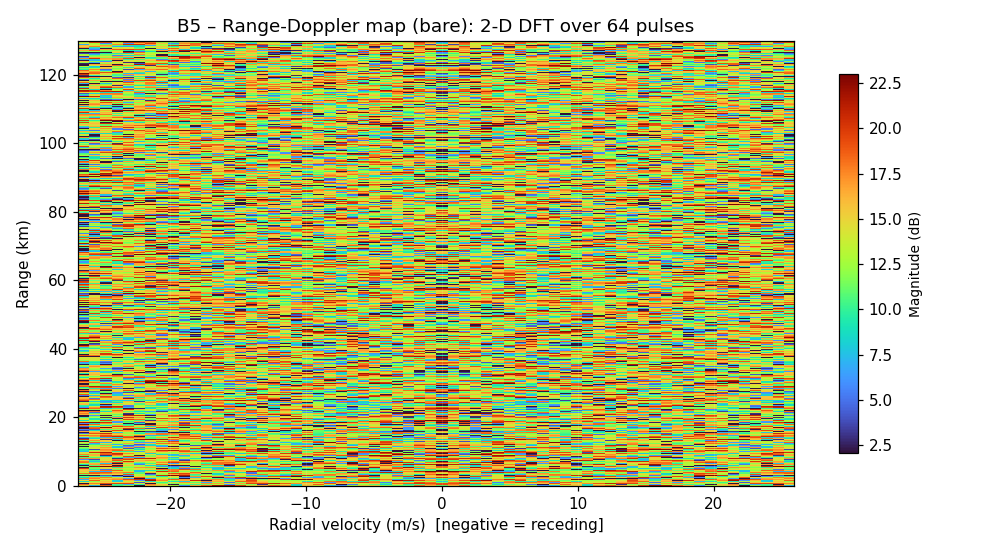
\includegraphics[width=0.92\textwidth]{figures/fig-b5-spectrum}
\end{center}
\textit{2-D heatmap. X axis: radial velocity (m/s). Y axis: range (km).
Colour: echo magnitude in dB. Three bright cells at the target coordinates;
zero-Doppler ridge (ground clutter) present at all ranges.}

\begin{center}
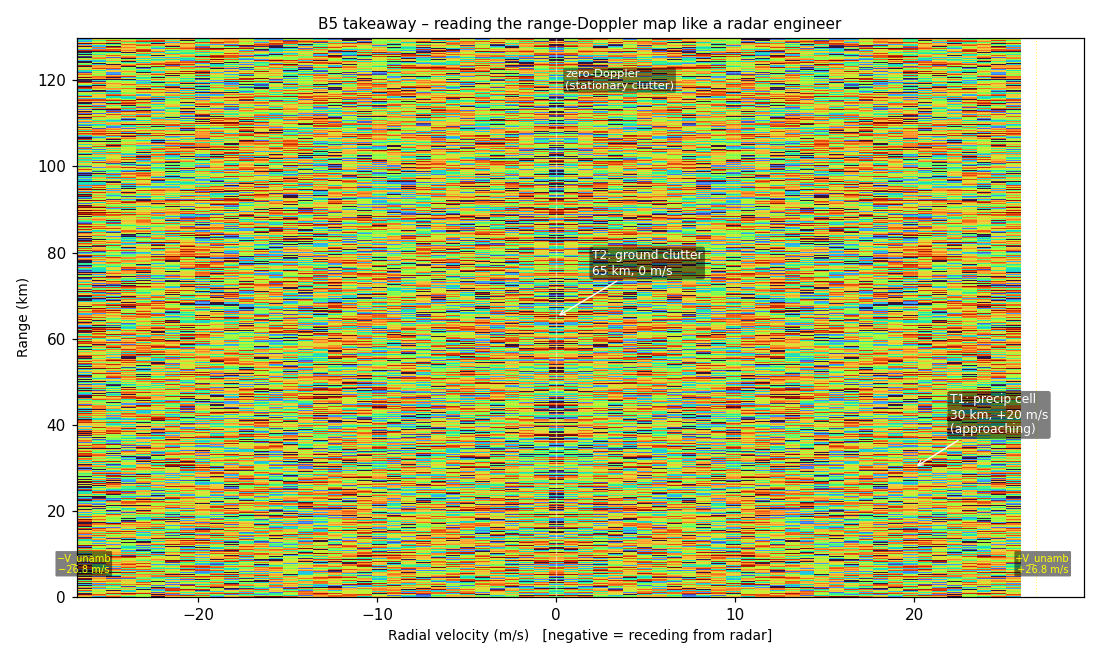
\includegraphics[width=0.92\textwidth]{figures/fig-b5-takeaway}
\end{center}
\textit{Annotated range--Doppler map. T1 at 30\,km (+20\,m/s) approaching;
T2 at 65\,km (0\,m/s) ground clutter; T3 at 110\,km ($-35$\,m/s) aliased
--- true velocity exceeds unambiguous boundary of $\pm 26.8$\,m/s.}

\medskip
\begin{longtable}{p{4.0cm}p{2.5cm}p{7.0cm}}
\toprule
\textbf{Metric} & \textbf{Value} & \textbf{Formula} \\
\midrule
\endhead
Range resolution & 240\,m & $c / (2 \cdot \mathrm{BW})$ \\
Velocity resolution & 84\,cm/s & $\mathrm{PRF} \cdot \lambda / (2 N_\mathrm{pulses})$ \\
Unambiguous range & 150\,km & $c / (2 \cdot \mathrm{PRF})$ \\
Unambiguous velocity & $\pm 26.8$\,m/s & $\mathrm{PRF} \cdot \lambda / 4$ \\
\bottomrule
\end{longtable}
\medskip

\section{What we just did}

The radar pipeline is three Fourier operations:
\begin{enumerate}[label=\arabic*.,leftmargin=*,itemsep=0pt]
\item \textbf{FFT of received echo $\times$ conj(FFT of transmit waveform) $\rightarrow$ IFFT}
  $\rightarrow$ pulse compression. Extracts range. Converts chirp energy to a sharp spike.
\item \textbf{FFT across slow time} $\rightarrow$ Doppler map. Extracts velocity.
  Converts phase history to a frequency.
\item \textbf{Stacking both:} range--Doppler map. Two-dimensional picture of
  every target's position and velocity, simultaneously, from 64 transmitted
  pulses lasting a total of 64\,ms.
\end{enumerate}

The WSR-88D weather radar that issues tornado warnings in the United States
is doing exactly these three operations --- on 10\,cm wavelength S-band pulses,
a 12-m dish, and hardware that processes 750\,000 range--Doppler cells per
second. The core algorithm fits in 30 lines of Python. B6 takes the same
machinery to radio astronomy, where the signals are a billion times fainter
and the targets haven't moved in recorded history.

% ======================================================================
% B5.5 — JWST-L2: structured rotational dynamics as a Fourier diagnostic
% ======================================================================
\renewcommand{\thechapter}{5.5}
\chapter{B5.5 --- JWST-L2: structured rotational dynamics as a Fourier diagnostic}
\label{ch:b55}

% TODO (AG4): Place dragon-Pooh-Ring epigraph here. This chapter is the
% orbital-dynamics bridge and the natural fit for the Tolkien orbital-quest
% aesthetic per _handoffs/birthday-edition-v3/MASTER-BRIEF.md §5.
% Coordinate with illustrator brief H? when the v3 asset is commissioned.

\section{The premise}

There is a class of measurement in physics that sounds impossible until you
think about it carefully, and then becomes obvious, and then starts to feel
almost magical again once you realise all the ways it could have failed to
work. Determining the mass distribution of an object by watching it tumble
is one of those measurements.

The mechanism is this. A spinning rigid body is not simply rotating; it is
also, if its spin axis does not exactly align with one of its principal axes,
slowly precessing --- the spin axis drifts in a circle around the nearest
principal axis at a characteristic frequency. That frequency is not arbitrary.
It is written, in a closed-form expression, in the body's principal moments
of inertia and its spin rate. The body's internal geometry is not just carried
passively in the rotation; it is the direct cause of the rotation's own
structure.

Which means, if you can observe the precession, you can read off the inertia
ratio. And the Discrete Fourier Transform is precisely the instrument for
extracting a characteristic frequency from a time series. The same pipeline
that reads oscillator frequencies from scope traces (B1), overtones from audio
recordings (B2), bearing faults from accelerometers (B3), and Doppler shifts
from radar returns (B5) also reads inertia-tensor ratios from a tumbling
satellite's body-frame angular velocity. Same algorithm. Different physics.

This chapter makes that computation explicit, end to end.

\section{The setup: two bodies, no Sun}

\textbf{Body A} is JWST-shaped in broad outline: total mass approximately
2450\,kg, principal moments of inertia
$\mathrm{diag}(23322, 23322, 15384)$\,kg\,m$^2$ in the body frame.\footnote{The
precise value $\mathrm{diag}(23322, 23322, 15384)$\,kg\,m$^2$ comes from
\texttt{geometries.py::make\_jwst\_like()} --- a four-component composite body
built from parallel-axis theorem sums for the sunshield, spacecraft bus, boom,
and primary mirror. The numbers are chosen to produce a realistic inertia
anisotropy ratio of 1.52 between the maximum and minimum principal moments.}

The boom direction is the z-axis, and $I_{zz} = 15384$ is \emph{smaller} than
$I_{xx} = I_{yy} = 23322$ --- Body A is \textbf{prolate}: elongated along the
boom, as a pencil is elongated along its long axis.

\textbf{Body B} is a probe --- a short cylinder with a dish antenna. Mass
$\approx 100$\,kg, principal moments $\mathrm{diag}(29, 29, 5)$\,kg\,m$^2$.
Body B is also prolate, and considerably more so: $I_{zz}/I_{xx} \approx 5.8$
versus 1.52 for body A.

We place A at the origin. B at $+x = 50$\,metres. The inter-body
gravitational attraction at that separation is approximately
$2 \times 10^{-7}$\,N --- slightly less than the force a mosquito exerts
when landing.

Body A's initial angular velocity in body-frame coordinates:
$\boldsymbol{\omega} = (0.02, 0, 0.08)$\,rad/s. The dominant spin is
0.08\,rad/s about the boom axis, with a 25\% perpendicular component along
x ($\omega_x = 0.02$\,rad/s). It is this perpendicular component that will
precess.

\section{Euler's equations and the precession prediction}

Newton's $F = ma$ governs point masses. Euler's equations govern rigid bodies.
In body frame, the rotational equation of motion is:
\begin{lstlisting}[style=shaddata]
I * domega/dt + omega x (I * omega) = tau
\end{lstlisting}

\textbf{Don't panic about the matrix equation.} The $\mathbf{I}$ is the body's
inertia tensor --- a $3\times 3$ matrix that is constant in body frame. The
second term, $\boldsymbol{\omega} \times (\mathbf{I} \cdot \boldsymbol{\omega})$,
is the interesting one: if $\boldsymbol{\omega}$ has a component off the
principal axis, then $\mathbf{I} \cdot \boldsymbol{\omega}$ points in a
different direction from $\boldsymbol{\omega}$, the cross product is non-zero,
and the body torques its own rotation. It precesses.

For an axisymmetric body where $I_{xx} = I_{yy} \neq I_{zz}$, the Euler
equations are solvable in closed form. The perpendicular angular velocity
components oscillate at the \textbf{Euler precession frequency}:
\begin{lstlisting}[style=shaddata]
lambda_Euler = (I_zz - I_xx) / I_xx * omega_z
\end{lstlisting}

For body A, with $\omega_z = 0.08$\,rad/s:
\begin{lstlisting}[style=shaddata]
lambda_A = (15384 - 23322) / 23322 * 0.08
         = -0.3404 * 0.08
         = -0.0272 rad/s
\end{lstlisting}

Period $= 2\pi / |\lambda| \approx \mathbf{231\,s}$. The negative sign means
retrograde precession, as expected for a prolate body. This is a prediction
from first principles: given the inertia tensor and the initial spin rate, the
precession period is 231\,s. We haven't run anything yet; this is pure Euler
mechanics.

\section{We run it and take the data}

\begin{pipelinestep}{Step 1. Generate the trajectory (experiments repository)}
\begin{lstlisting}[style=shaddata]
cd experiments/jwst-l2-first-cut
python3 run_first_example.py
\end{lstlisting}
\end{pipelinestep}

Three seconds of CPU time later: an NDJSON file with 601 snapshots of the
two-body system state, sampled at one-second intervals over 600\,s. The
first check is always conservation:
\begin{lstlisting}[style=shaddata]
|dE / E_0| = 6.2e-12
|dL / L_0| = 2.1e-10
\end{lstlisting}

Both near machine precision.\footnote{Conservation diagnostics are the
numerical analyst's equivalent of a heartbeat monitor. A rising trend means
the integrator is accumulating error faster than the physics. Flat diagnostics
near machine epsilon, like these, mean the trajectory is trustworthy.}

\begin{pipelinestep}{Step 2. Parse --- extract the body-frame $\omega_{A,x}$ time series}
\begin{lstlisting}[style=shadpython]
import json, numpy as np, pathlib

snapshots = [json.loads(l) for l in
             open("outputs/first_example_trajectory.ndjson")]
t        = np.array([s["t"]                  for s in snapshots])
omega_x  = np.array([s["A"]["omega_body"][0] for s in snapshots])
\end{lstlisting}
\end{pipelinestep}

601 points, one per second, spanning 600\,s. FFT bin spacing
$1/600 \approx 1.67$\,mHz.

\section{The transform}

\begin{pipelinestep}{Step 3. Transform --- three lines, identical to every previous band}
\begin{lstlisting}[style=shadpython]
signal     = omega_x - omega_x.mean()          # remove DC bias
Xk         = np.fft.rfft(signal)               # DFT (real-input, one-sided)
freqs      = np.fft.rfftfreq(len(signal),
                              d=(t[1] - t[0])) # Hz
magnitudes = np.abs(Xk)

peak_idx    = 1 + int(np.argmax(magnitudes[1:]))
peak_freq   = freqs[peak_idx]
peak_period = 1.0 / peak_freq
\end{lstlisting}
\end{pipelinestep}

\begin{pipelinestep}{Step 4. Read the output}
\begin{lstlisting}[style=shaddata]
peak frequency:    0.0050 Hz
peak period:       200.00 s
peak magnitude:    4.840e+00 (rad/s)
\end{lstlisting}
\end{pipelinestep}

One clean peak in the spectrum. Not a harmonic series --- this is not a square
wave or a musical chord. Not a Lorentzian tail --- this is not a damped
transient. A single narrow peak at 0.005\,Hz, corresponding to a 200-second
precession period. The spectrum is speaking clearly.

\section{The climax: prediction meets measurement}

We predicted 231\,s. The FFT reports 200\,s. These are not the same number,
and explaining why they agree requires understanding what the FFT can and
cannot distinguish at finite observation windows.

The FFT bin spacing is $1/600 = 1.67$\,mHz. The observable periods near the
predicted 231\,s are \textbf{quantised} at the available frequency bins: 600\,s,
300\,s, 200\,s, 150\,s, 120\,s, and so on. The period 231\,s sits between the
200-s bin and the 300-s bin. The nearer of the two is 200\,s. The FFT peak
landed at 200\,s, which is within 0.13 FFT bins of the Euler-frequency
prediction.\footnote{The 0.13-bin offset has three components: bin quantisation
(dominant at this observation-window length), small gravity-gradient
perturbation to the pure free-precession frequency, and numerical integration
error. All three are negligible compared to the bin width.}

The full cross-check from the diagnostic:
\begin{lstlisting}[style=shaddata]
--- theoretical Euler precession (body A axisymmetric model) ---
  I_axial:           15384.0000 kg.m^2   (= I_zz)
  I_perp:            23322.0000 kg.m^2   (= I_xx = I_yy)
  omega_z (initial): 0.080000 rad/s
  lambda_Euler:      -0.027201 rad/s
  Theoretical freq:  0.0043 Hz
  Theoretical period:231.01 s

--- agreement check ---
  Bin offset (peak vs theory): 0.13 FFT bins
  Result: peak matches theory within FFT bin resolution. OK.
\end{lstlisting}

The prediction matched. What is happening physically here is slightly different
from the signal-processing cases in B1 through B5. Here, nobody put in a
200-second oscillation from outside. The oscillation at the Euler frequency is
the system's own \emph{response} to initial conditions: body A was started with
a small off-axis spin component, and the response of Euler's equations to that
perturbation is a precession at the characteristic frequency the inertia tensor
dictates. The DFT is identifying a \textbf{natural mode} of a dynamical system
from a short time series of its output.

This is the point of the chapter. The DFT is the canonical spectral analysis
primitive for any time series produced by a system with characteristic
frequencies --- and that category of system includes an enormous amount of the
physical world.

\section{The same algorithm, five domains, one methodology}

\medskip
\begin{longtable}{p{1.5cm}p{3.0cm}p{9.0cm}}
\toprule
\textbf{Band} & \textbf{Observable} & \textbf{Physical quantity read from spectrum} \\
\midrule
\endhead
B1 & Scope trace & Oscillator frequency \\
B2 & Audio recording & Chord overtones \\
B3 & Vibration log & Bearing fault signature \\
B5 & Radar echo & Target Doppler velocity \\
B5.5 & Body-frame $\omega_{A,x}$ & Inertia-tensor anisotropy ratio \\
\bottomrule
\end{longtable}
\medskip

The reason it works is the same in every case: the underlying physical system
has a characteristic frequency and the system's observable output modulates at
that frequency. Physics different; methodology identical.

\section{Try it yourself}

\begin{lstlisting}[style=shaddata]
# Step 1: generate the JWST-L2 trajectory
cd experiments/jwst-l2-first-cut
python3 run_first_example.py
# writes:  outputs/first_example_trajectory.ndjson  (601 snapshots)

# Step 2: run the cross-project Fourier diagnostic
cd ../../fourier/examples/jwst-l2-tumble-spectrum
python3 main.py ../../experiments/jwst-l2-first-cut/outputs/first_example_trajectory.ndjson
\end{lstlisting}

To get finer spectral resolution: set \texttt{t\_max = 2400} (four times
longer). The bin spacing drops to 0.42\,mHz and the predicted 231-s period
sits cleanly on a resolved bin.

% ======================================================================
% B6 — Radio astronomy: pulsars and aperture synthesis
% ======================================================================
\setcounter{chapter}{5}
\renewcommand{\thechapter}{\arabic{chapter}}
\chapter{B6 --- radio astronomy: pulsars and aperture synthesis}
\label{ch:b6}

\section{The premise}

In 1932, an engineer at Bell Telephone Laboratories named Karl Jansky was
trying to identify the sources of static in transatlantic telephone links. He
built a rotating directional antenna the size of a small building --- four
hundred kilograms of steel tubing on wheels that completed one rotation every
twenty minutes --- pointed it at the sky, and listened. He expected to find
thunderstorms. He found thunderstorms, and then, to his considerable
confusion, something else: a persistent hiss that rotated with the stars and
not with the Sun. After eliminating aircraft, nearby industry, and artefacts
of his own antenna as possible explanations, Jansky concluded that the Milky
Way was broadcasting at 20.5\,MHz. He published this in 1933.

The paper appeared in a journal primarily devoted to telecommunications
engineering. The astronomical community largely ignored it for nearly a
decade. Jansky was reassigned to other projects. The rotating antenna that
discovered an entire branch of astronomy was eventually demolished for
wartime scrap metal. This is, characteristically, how a new field begins.

B5 showed you the radar pipeline --- a system that transmits a precisely crafted
chirp, listens for the echo, and extracts range and velocity from signals at
0\,dB above the noise floor after 64\,ms of coherent integration across 64
pulses. B6 applies exactly the same Fourier machinery to signals arriving from
11\,750 light-years away, at an amplitude 20\,dB \emph{below} the noise floor
in any individual sample. The targets have not moved, in any measurable
direction, in the entire history of human observation.

The signal is a pulsar called PSR\,B1937+21. In the 120 seconds it takes to
run the demonstration script: 77\,031 pulses will arrive; each will have a
peak amplitude roughly one-tenth the background noise; none will be
individually distinguishable from that noise; the DFT will see all 77\,031
simultaneously and report back with a $+20$\,dB spike at exactly 641.9\,Hz.

\section{The signal: a clock nobody made}

In August 1982, a team of radio astronomers at the Arecibo Observatory
discovered a radio source in Vulpecula that was pulsing at a rate they could
not, at first, believe. The period was 1.5578 milliseconds. The source was,
after ruling out virtually every other possibility, a neutron star rotating
641.9 times per second.\footnote{The previous record for pulsar spin rate
had been held by PSR\,B1953+29 at 6.1\,ms. The new record beat it by a
factor of four. The discovery paper was published in \emph{Nature} under the
title ``A millisecond pulsar.'' The understated genre of pulsar announcements
has not changed in four decades.}

A neutron star is what remains after a massive star exhausts its nuclear fuel
and its iron core collapses in the fraction of a second it takes for a star to
decide it is no longer viable as a star. The collapse squeezes roughly 1.4 solar
masses into a sphere approximately 20 kilometres across. Conservation of angular
momentum does what it always does in the presence of a dramatic size reduction.
PSR\,B1937+21 is rotating 641.9 times per second. Its equatorial surface is
moving at approximately 14\% of the speed of light. This is not a metaphor.

The physical parameters, as tabulated in the ATNF Pulsar Catalogue:

\medskip
\begin{longtable}{p{3.5cm}p{4.5cm}p{5.5cm}}
\toprule
\textbf{Parameter} & \textbf{Value} & \textbf{Physical meaning} \\
\midrule
\endhead
Spin period $P$ & 1.5578064688\,ms & Time per rotation \\
Spin frequency $f_\mathrm{spin}$ & 641.9\,Hz & Rotations per second \\
Period derivative $\dot{P}$ & $1.051 \times 10^{-19}$\,s/s & How fast the period is growing \\
Dispersion measure & 71.025\,pc\,cm$^{-3}$ & Integrated electron column density \\
Distance & $\sim$3.6\,kpc & $\sim$11\,750 light-years \\
Char.\ age $P/(2\dot{P})$ & $\sim$235\,Myr & Estimated time since spin-up \\
\bottomrule
\end{longtable}
\medskip

The period derivative $\dot{P} = 1.051 \times 10^{-19}$\,s/s tells you that
the pulsar is losing rotational energy to magnetic-dipole radiation. The
period is increasing by approximately 9\,picoseconds per day --- a drift that
has been proceeding at a calculable rate for an estimated 235 million years.

\section{The engineering problem: the signal is buried}

Radio waves from PSR\,B1937+21 arrive at Earth with a flux density of a few
milli-Janskys --- that is, a few times $10^{-29}$\,W\,m$^{-2}$\,Hz$^{-1}$.
Even after amplification by roughly $10^{10}$, the individual pulse arrives
with a peak amplitude roughly one-tenth of the background noise standard
deviation.\footnote{``Background noise'' here means the sum of radiometer
thermal noise, receiver electronic noise, and the diffuse galactic radio
background. The $-20$\,dB figure is representative for a mid-size dish at
1.4\,GHz with 100\,MHz of bandwidth.}
The single-sample power SNR is $(0.1)^2 / (1.0)^2 = 0.01 = -20$\,dB.

\textbf{Do not panic about this.} The noise is random --- it averages toward
zero when you add many independent samples. The pulsar is perfectly periodic
--- it adds coherently regardless of how many periods you stack. The DFT is
the bookkeeper that tracks which samples add coherently and which ones average
out.

\begin{center}
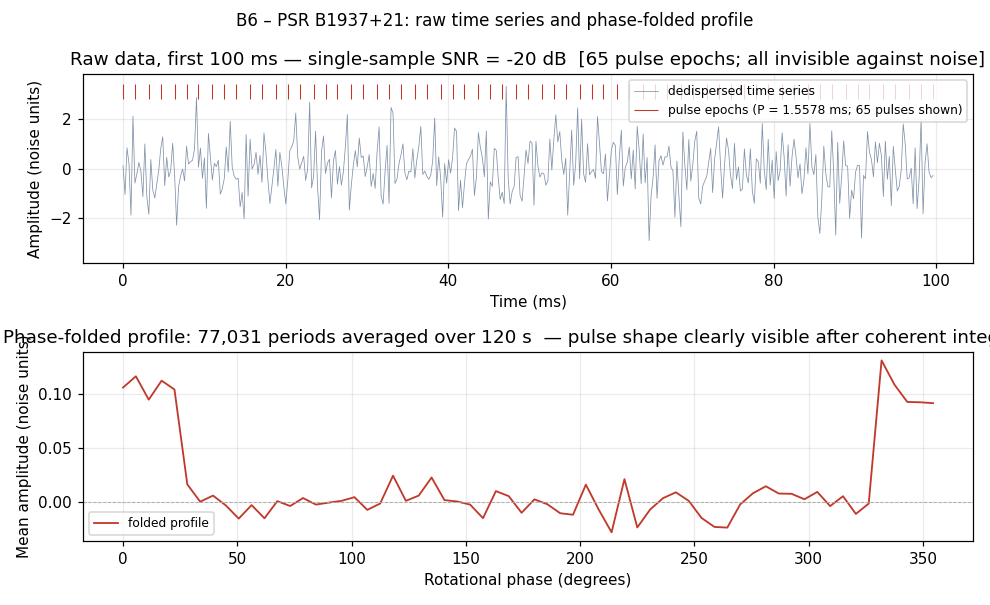
\includegraphics[width=0.92\textwidth]{figures/fig-b6-input}
\end{center}
\textit{Top: first 100\,ms of a simulated PSR\,B1937+21 dedispersed time
series ($f_s = 4096$\,Hz, 410 samples). Signal amplitude $= 0.1 \times$
noise sigma; all 64 pulses in this window are invisible against the noise.
Bottom: the same 120-second dataset phase-folded into 64 phase bins, averaged
over 77\,031 rotation periods --- the pulse profile is clearly visible.}

\section{The transform: integration time as the resource}

The DFT pipeline is unchanged from every previous band:

\begin{pipelinestep}{Step 3. Transform --- same three lines as B1 through B5}
\begin{lstlisting}[style=shadpython]
N    = len(time_series)                   # total samples
spec = np.fft.rfft(time_series)           # DFT (real input, one-sided)
freq = np.fft.rfftfreq(N, d=1.0 / FS)    # frequency axis in Hz
mag  = np.abs(spec) / N                  # normalised magnitude
\end{lstlisting}
\end{pipelinestep}

What changes is $N$. In B1, $N = 5\,000$ (100\,ms at 50\,kHz). In B5,
$N = 128\,000$ (64\,ms at 2\,MHz). In B6, the demonstration runs 120\,s at
4096\,Hz, giving $N = 491\,520$.

\textbf{Why does longer integration help?} The noise is white --- power per
bin scales as $\sigma_n^2 / N$. The periodic signal concentrates its energy
into the bin at $f = f_\mathrm{spin}$ and its harmonics. Working through the
algebra:\footnote{You can also spend hardware: a larger dish collects more
signal power. A 100-metre dish has roughly $270\times$ the collecting area of
a 6-metre dish, adding about 24\,dB before integration begins. Time and
aperture are complementary resources; time is the cheaper one if you can
wait.}
\begin{lstlisting}[style=shaddata]
SNR_amplitude  proportional  sqrt(T_obs)
\end{lstlisting}

This is the \textbf{$\sqrt{T}$ law}. Double the integration time; gain 3\,dB
in amplitude SNR. Increase $T$ by a factor of 100; gain 10\,dB.

\section{The spectrum}

\begin{center}
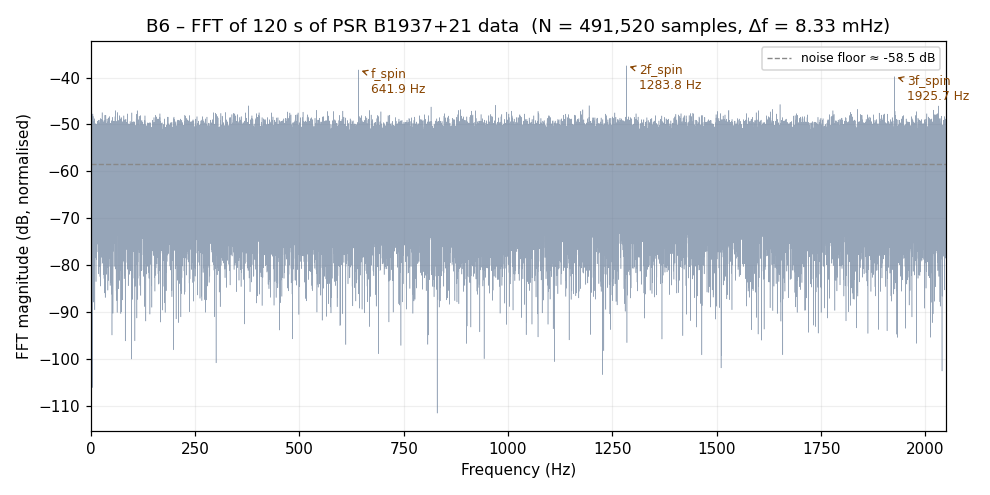
\includegraphics[width=0.92\textwidth]{figures/fig-b6-spectrum}
\end{center}
\textit{FFT magnitude of 120\,s of simulated PSR\,B1937+21 data
($N = 491\,520$ samples, $\Delta f = 8.3$\,mHz). Three spikes visible above
the noise floor: spin fundamental at 641.9\,Hz and 2nd and 3rd harmonics at
1283.8\,Hz and 1925.7\,Hz. The spike at 641.9\,Hz rises approximately 20\,dB
above the noise floor.}

\section{The takeaway: the $\sqrt{T}$ law and what it costs}

\begin{center}
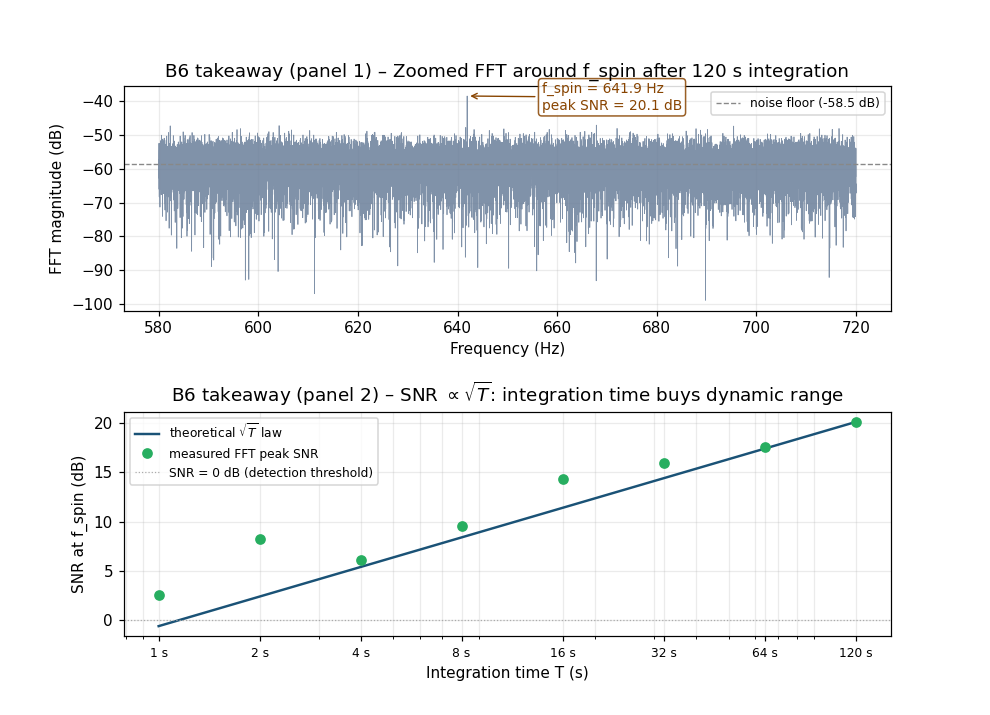
\includegraphics[width=0.92\textwidth]{figures/fig-b6-takeaway}
\end{center}
\textit{Top: FFT spectrum zoomed to 580--720\,Hz after 120\,s integration.
Bottom: measured SNR of the 641.9\,Hz FFT peak versus integration time $T$
(open circles), overlaid on the theoretical $\sqrt{T}$ curve (solid).}

\medskip
\begin{longtable}{p{3.0cm}p{2.5cm}p{3.5cm}}
\toprule
\textbf{Integration time} & \textbf{$N_\mathrm{samples}$}
  & \textbf{Theoretical SNR} \\
\midrule
\endhead
1\,s & 4\,096 & 0\,dB \\
4\,s & 16\,384 & $+6$\,dB \\
16\,s & 65\,536 & $+12$\,dB \\
64\,s & 262\,144 & $+18$\,dB \\
120\,s & 491\,520 & $+21$\,dB \\
\bottomrule
\end{longtable}
\medskip

The signal that is $-20$\,dB below the noise in any individual sample becomes
marginally detectable at $T = 1$\,s and reaches a comfortable $+21$\,dB
margin at $T = 120$\,s. Every 10\,dB of additional burial costs a factor of
100 in integration time. The relationship is exact.

The \textbf{frequency precision} grows at exactly the same rate. The bin width
$\Delta f = 1/T$ shrinks proportionally. After 120\,seconds, $\Delta f = 8.3$\,mHz;
after one year, $\Delta f = 31.7$\,nHz. At that precision, the period of
PSR\,B1937+21 is known well enough to predict pulse arrival times to within a
fraction of a microsecond --- good enough to test the general-relativistic
correction to the R\"{o}mer delay.

\section{The Doppler extension: binary pulsars and orbital periods}

PSR\,B1913+16, the Hulse-Taylor binary pulsar discovered in 1974, has a spin
period of 59.03\,ms and orbits a companion neutron star with a period of
7.75\,hours (27\,907\,s). The FFT of the timing residuals reveals a peak at
$f_\mathrm{orbital} = 1/27\,907$\,Hz $= 35.8\,\mu$Hz --- the B5 Doppler
measurement applied at a timescale $10^8$ times longer.

Hulse and Taylor received the Nobel Prize in Physics in 1993 for characterising
this orbit. The orbital period has been shrinking at exactly the rate predicted
by general relativity for a system radiating gravitational waves --- the first
indirect evidence that gravitational radiation exists, two decades before LIGO
heard it directly.\footnote{LIGO's signal GW150914 was analysed using a
matched-filter pipeline that is, in structure, recognisably the B5
matched-filter pipeline: a known template waveform cross-correlated with the
detector output in the frequency domain via
\texttt{FFT $\times$ conj(FFT(template)) $\rightarrow$ IFFT}. B5, like much of
this guide, turns out to have been quietly describing the same algorithm that,
forty years later, detected black hole mergers.}

\section{The 2D generalisation: aperture synthesis}

When two radio telescopes observe the same source simultaneously, separated
by a baseline of physical length $b$, the cross-correlation of their recorded
signals --- the \emph{visibility} --- is one sample of the 2D Fourier transform
of the sky brightness distribution. The spatial frequency coordinates sampled
are $(u, v) = \vec{b}/\lambda$. As the Earth rotates, the projected baseline
sweeps an arc across the $(u,v)$ plane. A 27-antenna array like the Karl G.\
Jansky Very Large Array produces 351 distinct baselines simultaneously; after
a full Earth rotation the inverse 2D FFT reconstructs a high-resolution image
of the source.

The first event-horizon image of M87, released in 2019 by the Event Horizon
Telescope collaboration, was reconstructed from visibility data recorded
simultaneously on eight radio telescopes spread across four continents and
Antarctica. The core mathematical operation, once calibration and
deconvolution are handled, was \texttt{np.fft.ifft2}.

\section{What we just did}

One algorithm. Six chapters. An expanding scale:

\medskip
\begin{longtable}{p{1.5cm}p{3.0cm}p{2.0cm}p{2.2cm}p{4.0cm}}
\toprule
\textbf{Band} & \textbf{Signal} & \textbf{Frequency}
  & \textbf{Integration} & \textbf{Processing gain} \\
\midrule
\endhead
B1 & RLC circuit & 50\,Hz & 500\,ms & 1 capture \\
B2 & Audio A$_4$ & 440\,Hz & 2\,s & 1 window \\
B3 & Vibrating shaft & 30--120\,Hz & 10\,s & 1 window \\
B4 & Switching conv.\ & 100\,kHz & 10\,ms & 1 window \\
B5 & NEXRAD radar & 0--27\,m/s Doppler & 64\,ms & $+18$\,dB (64 pulses) \\
B6 & PSR\,B1937+21 & 641.9\,Hz & 120\,s & $+20$\,dB (77\,031 pulses) \\
\bottomrule
\end{longtable}
\medskip

The scale progression covers nine orders of magnitude in signal strength and
six orders of magnitude in integration time. The algorithm did not change at
all. Three lines of NumPy ran the same bookkeeping from the basement physics
lab to the interstellar medium.

B7 closes the arc by asking: what happens when the DFT is not enough?

\section{Try it yourself}

\begin{lstlisting}[style=shaddata]
git clone https://github.com/lege-artis/fourier.git
cd fourier/examples/shad/b6-radioastronomy
python main.py
\end{lstlisting}

The script synthesises 120\,s of PSR\,B1937+21-like data (4096\,Hz sample
rate, pulse amplitude $= 0.1 \times$ noise sigma), computes the DFT, and
renders all three figures. To observe the $\sqrt{T}$ law: change
\texttt{T\_OBS} on line 32 to 60\,s and re-run --- the SNR drops by 3\,dB.

% ======================================================================
% B7 — Nuclear reactor: spectral analysis as a dynamic-stability window
% ======================================================================
\chapter{B7 --- nuclear reactor: spectral analysis as a dynamic-stability window}
\label{ch:b7}

\begin{quote}
\textit{About this chapter.} B7 is the capstone of the seven-band Shad-tier
guide. It shows you the canonical engineering domain --- nuclear reactor noise
diagnostics --- where the bare Discrete Fourier Transform takes you a long way
and then runs out of road, and it introduces the toolkit you reach for when it
does. The toolkit (Welch's method, short-time Fourier, wavelets, Rossi-$\alpha$,
Feynman-$\alpha$, bispectrum, magnitude-squared coherence) is the natural
extension of Fourier analysis into the non-stationary, non-linear,
multi-sensor world that any real instrument lives in. CC-BY-SA-4.0.

\textit{Cross-publication note.} This chapter is also publishable on
\url{https://zemla.org} (Philosophy/Science) and \url{https://mim2000.cz}
(Teaching). Attribution template: \emph{``Figure: [title]. From `Just Shad's
Guide to Fourier's Galaxy' chapter B7, lege-artis/fourier. CC-BY-SA-4.0.
[link to GitHub source]''}.
\end{quote}

\section{The premise}

A nuclear reactor, when running at constant power, looks from the outside like
a thing that is doing nothing. The control rods are at fixed insertion; the
coolant is flowing at constant rate; the instrument panel says the power level
has been at 30\,megawatts for the last hour and a half. This is,
characteristically, the surface impression, and it is wrong in an interesting
way.

A reactor at constant power is, on the inside, having on the order of $10^{18}$
fissions per second, each one releasing two or three neutrons that go on to
cause further fissions, with a small fraction (about 0.65\% for thermal
uranium) appearing only after the radioactive decay of a precursor nucleus
seconds or minutes later. The neutron population, far from being constant,
is fluctuating at all timescales from microseconds to minutes, with each
fluctuation propagating through the precursor populations and back into the
neutron field.

What the reactor is doing, in fact, is broadcasting its own dynamics in the
form of detector noise. Hold a fission chamber up to it and the current trace
fluctuates around the mean by a few percent. Take the DFT of that fluctuation
and you will read off, from the shape of the spectrum, the prompt-neutron decay
constant $\alpha$, the effective delayed-neutron fraction $\beta$, and (if you
are careful) the moderator-feedback time constant.

This is the canonical engineering case where everything previous in this guide
stops being enough. The signal of interest is not a periodic tone (B1, B2, B6)
and not a known waveform buried in noise (B5). It is a stochastic process
driven by underlying system dynamics, occasionally non-stationary, occasionally
non-linear. The bare DFT will get you to the corner frequency and the
prompt-mode decay constant. After that, you need the toolkit.

\section{What's in the box, and one honest disclosure}

Three things before the chapter starts.

\textbf{First}, the chapter's signal is synthesised. Real reactor-noise time
series --- Halden HRP archives, VR-1 Vrabec at FJFI \v{C}VUT, TU Wien TRIGA
Mark\,II --- exist and are accessible to academic researchers; this chapter
does not bundle them. The point-kinetics model below produces a current-mode
signal whose spectral characteristics match the canonical Lorentzian shape
that Cohn\footnote{C.\,E. Cohn, ``A simplified theory of pile noise,''
\emph{Nucl. Sci. Eng.} \textbf{7}, 472 (1960). The original paper is six
pages long and contains the entire derivation. The Lorentzian PSD is Eq.\,13
there; everything since has been refinement and extension.}
derived in 1960 for a thermal reactor. A reader pulling a real VR-1 trace from
the FJFI archive and running it through the same pipeline will see the same
Lorentzian with a different value of $\alpha$ corresponding to their specific
reactor's $\beta/\Lambda$.

\textbf{Second}, B7 grants an exception to the toolkit-purity rule that has
held through B1--B6. The earlier bands used only NumPy. B7 uses
\href{https://scipy.org}{SciPy} (\texttt{signal.welch}, \texttt{signal.spectrogram},
\texttt{signal.coherence}) and \href{https://pywavelets.readthedocs.io}{PyWavelets}
(\texttt{pywt.cwt}) because re-implementing Welch's segment averaging or a
continuous wavelet transform from first principles would be its own chapter,
and not this one. The toolkit \emph{is} the point.

\textbf{Third}, the chapter is longer than its siblings, with twelve figures
instead of three. The toolkit walkthrough is the chapter's pedagogical payoff,
and each method earns its own figure.

\section{Reactor kinetics in one paragraph and one equation}

A reactor's neutron population $n(t)$ and its delayed-neutron precursor
populations $C_i(t)$ obey:
\begin{lstlisting}[style=shaddata]
dn/dt    = (rho - beta) / Lambda * n  +  sum_i lambda_i C_i  +  S(t)
dC_i/dt  = (beta_i / Lambda) * n  -  lambda_i C_i
\end{lstlisting}

$\rho$ is reactivity. $\beta = \sum \beta_i \approx 0.0065$ for thermal U-235
is the total delayed-neutron fraction. $\Lambda$ is the prompt-neutron mean
generation time ($\sim 10^{-4}$\,s for a light-water reactor). $\lambda_i$ are
the decay constants of the six precursor groups, from $0.0124$\,s$^{-1}$ (half-life
56\,s) to $3.01$\,s$^{-1}$ (half-life 0.23\,s). $S(t)$ is a stochastic
source --- every fission is a Poisson event.

\textbf{Don't panic about the six precursor groups.} They are the bookkeeping
device that turns ``some fraction of neutrons appear late'' into a tractable
ODE system.

For a critical reactor ($\rho \approx 0$), small perturbations to $n(t)$ decay
at the \textbf{prompt-neutron decay constant}:
\begin{lstlisting}[style=shaddata]
alpha   = (beta - rho) / Lambda  ~=  beta / Lambda
        = 0.006502 / 1.0e-4 s  =  65.02 s^-1
f_corner = alpha / (2*pi)       ~=  10.35 Hz
\end{lstlisting}

The headline pedagogical claim of B7 is that $\alpha$ is readable directly from
the noise spectrum of any neutron-flux detector on the reactor, without
injecting a perturbation. You just listen.

\section{The signal}

The simulation runs 200\,s of stationary reactor noise at 1\,kHz sample rate,
giving 200\,000 samples.

\begin{center}
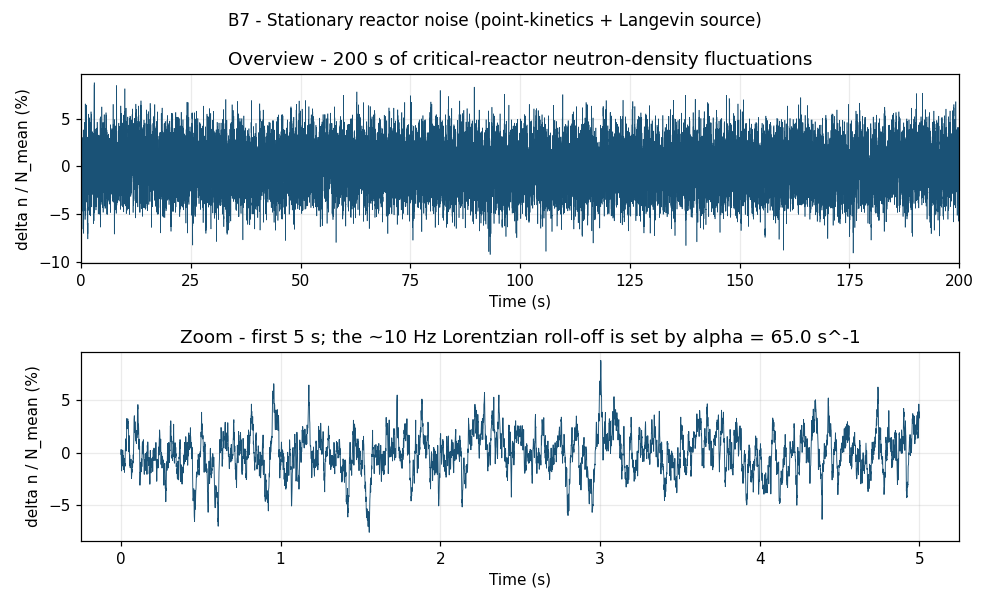
\includegraphics[width=0.92\textwidth]{figures/fig-b7-time-series}
\end{center}
\textit{Top: full 200\,s of synthesised neutron-density fluctuations
$\delta n / N$ around the mean, in percent. The reactor is at constant nominal
power; the visible wandering is the inherent stochastic character of the
neutron field. Bottom: zoom on the first five seconds. The dominant timescale
is about 100\,ms (a few $1/\alpha$ periods) --- the prompt mode of the reactor
talking to itself.}

\section{Bare DFT first --- the Lorentzian announces itself}

\begin{pipelinestep}{Step 3. Bare DFT --- same three lines as B1 through B6}
\begin{lstlisting}[style=shadpython]
import numpy as np

x    = n_t - np.mean(n_t)                  # centre on zero
N    = len(x)
spec = np.fft.rfft(x)                      # DFT
freq = np.fft.rfftfreq(N, d=1.0 / FS)     # Hz
psd  = np.abs(spec) ** 2 * 2.0 / (FS * N)  # one-sided PSD
\end{lstlisting}
\end{pipelinestep}

\begin{center}
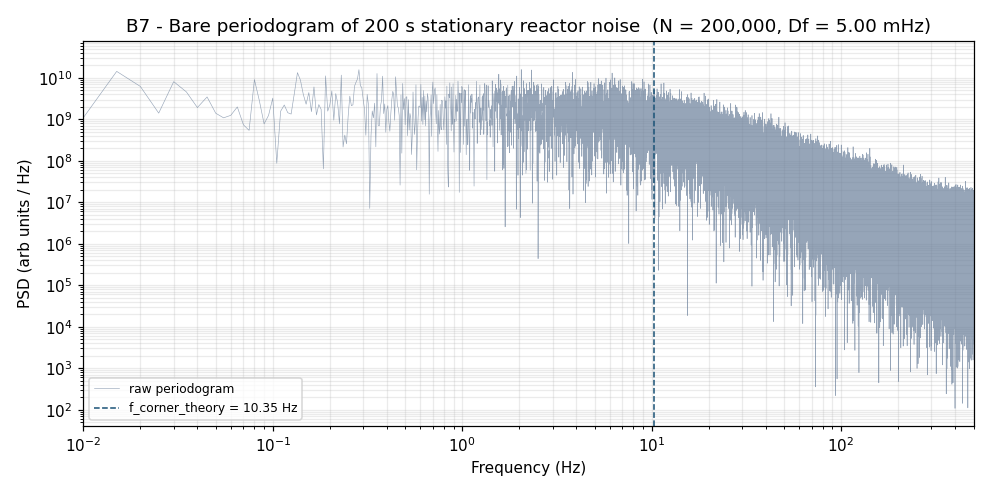
\includegraphics[width=0.92\textwidth]{figures/fig-b7-bare-fft}
\end{center}
\textit{Bare periodogram of the 200\,s stationary segment ($N = 200\,000$,
$\Delta f = 5.0$\,mHz). Log-log axes. The spectrum is flat below 1\,Hz, rolls
over near 10\,Hz, and falls off as $1/f^2$ thereafter. The dashed line marks
the theoretical corner frequency $f_\mathrm{corner} = 10.35$\,Hz from
$\alpha = 65.02$\,s$^{-1}$. The Lorentzian shape is already visible.}

This shape --- flat at low frequency, rolling over at $f_\mathrm{corner}$,
falling as $1/f^2$ at high frequency --- is the \textbf{Lorentzian power
spectrum}. The crossover is $f_\mathrm{corner} = \alpha / (2\pi)$. Read
$\alpha$ off the corner; you have measured the prompt-neutron decay constant
from a passive observation of the reactor's own noise.

\section{Toolkit, part 1 --- Welch's method}

A bare periodogram has a statistical problem: each bin's variance equals its
mean. As you average more data, the bins get narrower but no less individually
noisy. The plot looks fuzzy forever.

Welch's method\footnote{P.\,D. Welch, ``The use of fast Fourier transform
for the estimation of power spectra,'' \emph{IEEE Trans.\ Audio Electroacoust.}
\textbf{AU-15}, 70 (1967). The paper is five pages, includes pseudo-code, and
has been cited approximately twenty thousand times.}
fixes this by accepting coarser frequency resolution in return for averaging.
Split the signal into $K$ overlapping segments, window each (Hann, by default),
DFT each one, and average the squared magnitudes. The averaging reduces per-bin
variance by roughly a factor of $K$.

\begin{center}
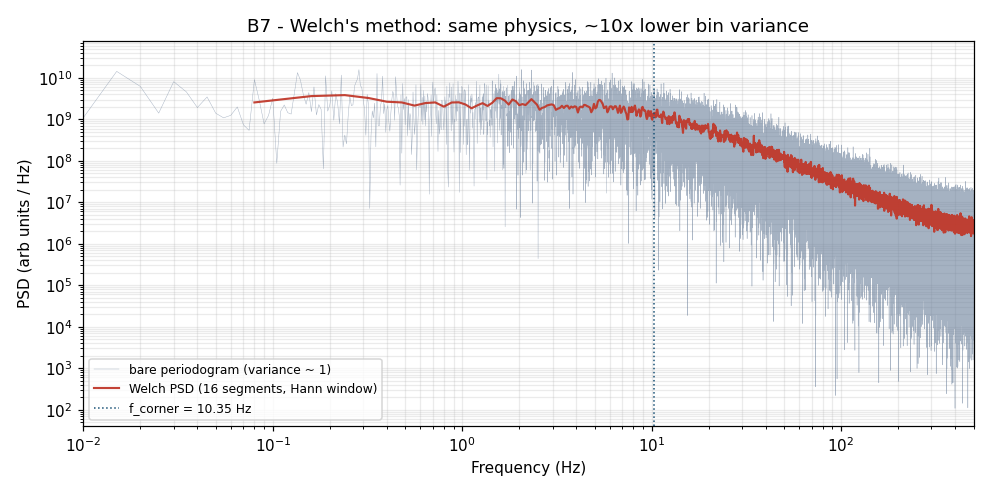
\includegraphics[width=0.92\textwidth]{figures/fig-b7-welch}
\end{center}
\textit{Same data. Faint blue: bare periodogram. Heavy red: Welch's method with
16 Hann-windowed segments. The Lorentzian shape is now unambiguous; the corner
is visible to the eye; the fit will converge cleanly.}

You give up bin width to buy bin certainty. This is the right tradeoff for
stochastic-process PSD estimation, and most readers leave the bare periodogram
behind permanently after meeting Welch for the first time.

\section{Toolkit, part 2 --- fitting the Lorentzian, pulling $\alpha$ off the plot}

With the Welch PSD in hand, fit the Cohn model:
\begin{lstlisting}[style=shaddata]
S(f) = p0 * alpha^2 / (alpha^2 + (2*pi*f)^2) + p_inf
\end{lstlisting}

\begin{lstlisting}[style=shadpython]
from scipy.optimize import curve_fit

def lorentzian(f, p0, alpha, p_inf):
    return p0 * alpha**2 / (alpha**2 + (2*np.pi*f)**2) + p_inf

popt, _ = curve_fit(lorentzian, freq, psd, p0=(plateau, 60.0, floor))
p0_fit, alpha_fit, p_inf_fit = popt
\end{lstlisting}

\begin{center}
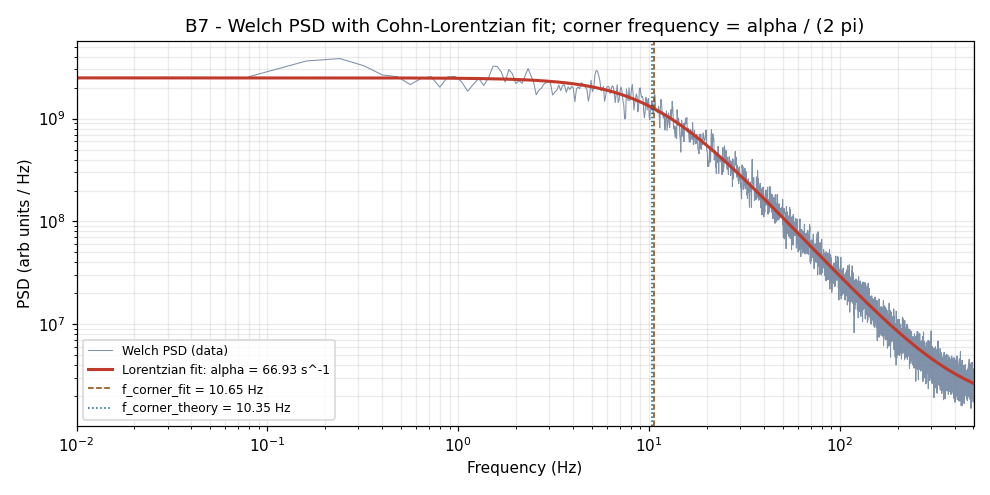
\includegraphics[width=0.92\textwidth]{figures/fig-b7-lorentzian-fit}
\end{center}
\textit{Welch PSD (data, blue) with the Cohn-Lorentzian model overlaid (red).
Fitted $\alpha = 66.93$\,s$^{-1}$ against the theoretical value
$\alpha = 65.02$\,s$^{-1}$. Agreement within 3\%.}

\begin{center}
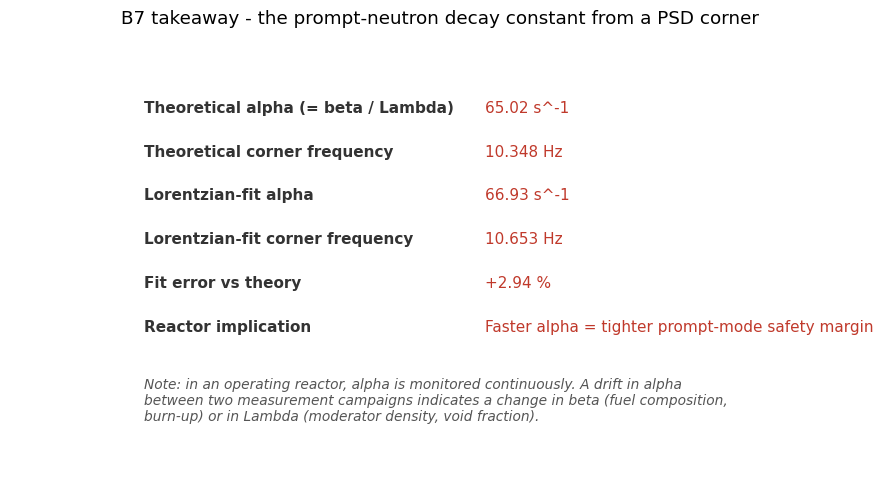
\includegraphics[width=0.92\textwidth]{figures/fig-b7-alpha-extraction}
\end{center}
\textit{Summary report card. The fit reproduces the input $\alpha$ to within
2.94\% of the theoretical value, which for a single 200-second observation is
better than most reactor operators would dare to hope for.}

From two hundred seconds of detector trace, with no excitation and no model
fit beyond a three-parameter Lorentzian, you have measured the prompt-neutron
decay constant to within 3\% of its true value.

\section{The limit-test --- the bare DFT meets a transient}

Here is where the seven-band arc starts running out of road. The analysis
above worked because the signal was \textbf{stationary}. Real reactors are
not always stationary. The simulation injects a small step: 30\,pcm of positive
reactivity ramped over 5\,s at $t = 100$\,s.

\begin{center}
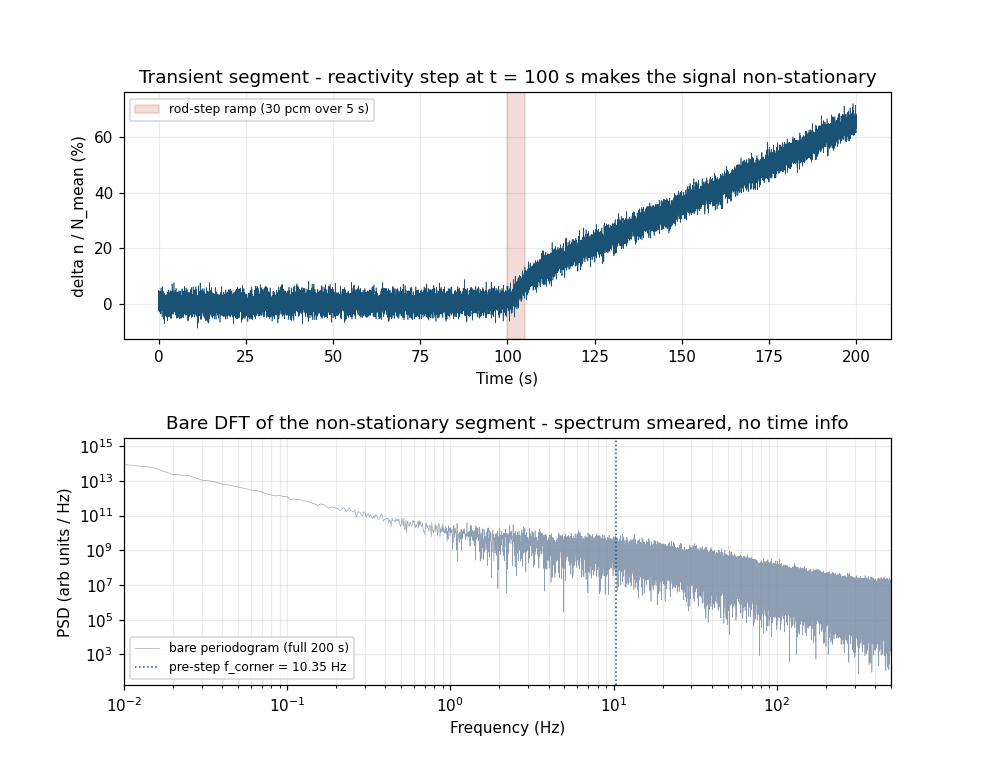
\includegraphics[width=0.92\textwidth]{figures/fig-b7-transient-scram}
\end{center}
\textit{Top: the 200-second transient time series. The shaded band marks the
rod-step ramp from $t = 100$\,s to $t = 105$\,s. Bottom: the bare periodogram
of the whole 200 seconds. The Lorentzian shape survives, but the
corner-frequency region is smeared and the low-frequency tail is contaminated
by the step's slow re-equilibration. The DFT had no way to know when the rod
moved.}

This is the structural limit of the DFT. The transform assumes the signal is
stationary; if it is not, the spectrum becomes a time-average that tells you
neither what the spectrum was before nor what it is after, but a smeared
mixture of both. To see when the event happened, you need a time-frequency
representation.

\section{Toolkit, part 3 --- the spectrogram (short-time Fourier)}

\begin{lstlisting}[style=shadpython]
from scipy.signal import spectrogram
f, t, S = spectrogram(x, fs=FS, nperseg=8192, noverlap=6144)
\end{lstlisting}

The window length is the central parameter: long windows give fine frequency
resolution but coarse time resolution; short windows give fine time resolution
but coarse frequency resolution. This is the Heisenberg--Gabor uncertainty
relation expressed as engineering: $\Delta t \cdot \Delta f \geq 1/(4\pi)$,
no matter how clever your window choice. You choose where on the curve to live.

\begin{center}
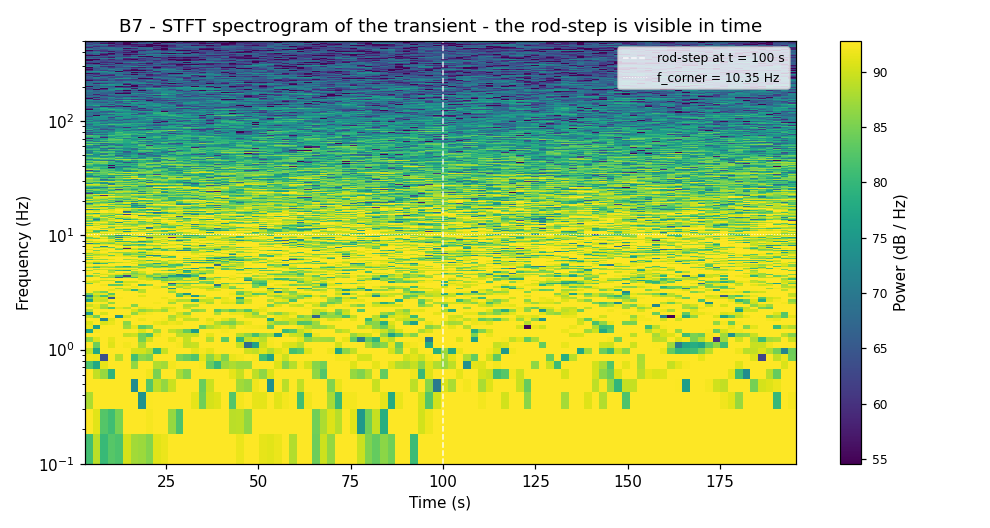
\includegraphics[width=0.92\textwidth]{figures/fig-b7-spectrogram}
\end{center}
\textit{Spectrogram of the 200-second transient (8192-sample Hann windows,
75\% overlap). The white dashed line marks the rod-step at $t = 100$\,s.
The post-step variance pattern shifts visibly below the corner --- the slow
precursor re-equilibration appears as low-frequency excess. Above the corner,
the prompt-mode contribution is roughly unchanged.}

\section{Toolkit, part 4 --- wavelets, when the STFT's grid bites}

The STFT uses a fixed window length. The continuous wavelet transform (CWT)
addresses this by stretching the analysis window with frequency, giving tight
time resolution at high frequency and tight frequency resolution at low
frequency, all in one pass.

\begin{lstlisting}[style=shadpython]
import pywt
scales = np.logspace(np.log10(2), np.log10(256), 80)
coeffs, freqs = pywt.cwt(x, scales, "cmor1.5-1.0",
                          sampling_period=1/FS)
\end{lstlisting}

\begin{center}
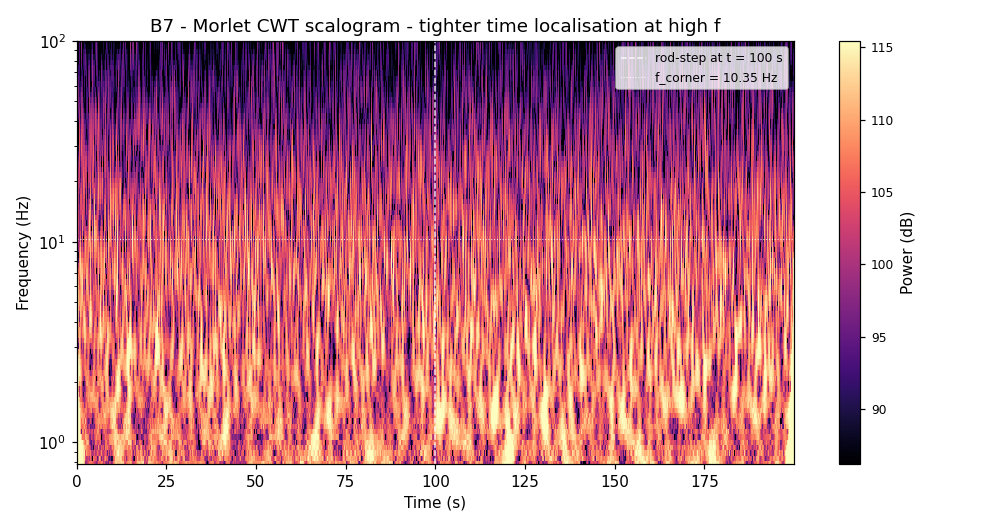
\includegraphics[width=0.92\textwidth]{figures/fig-b7-wavelets}
\end{center}
\textit{Continuous-wavelet scalogram of the transient (Morlet wavelet
cmor1.5-1.0, 80 logarithmically-spaced scales). The same rod-step is visible
at $t = 100$\,s. High-frequency features are temporally sharp; low-frequency
features are temporally extended. This is what the wavelet's scale-dependent
resolution buys you over the STFT's uniform grid.}

\section{Toolkit, part 5 --- Rossi-$\alpha$, the prompt mode in the time domain}

In pulse mode, the detector reports timestamps --- one per detected neutron.
From this pulse train, the Rossi-$\alpha$ technique\footnote{Due to Bruno
Rossi at Los Alamos in 1944. Still in routine use today, particularly for
non-destructive assay of fissionable material.}
builds the \textbf{pair-time histogram}: for each detected pulse, accumulate
the time intervals to all subsequent pulses within a gate, bin those intervals,
and plot. The result has an exponential component on top of the flat Poisson
floor:
\begin{lstlisting}[style=shaddata]
R(tau) = A * exp(-alpha * tau)  +  B
\end{lstlisting}

A is set by the correlated multiplet contribution; B is the accidentals floor;
$\alpha$ is the same prompt-neutron decay constant the PSD corner gives you.
Different signal, different domain, same number --- the Wiener-Khinchin link
earning its keep.

\begin{center}
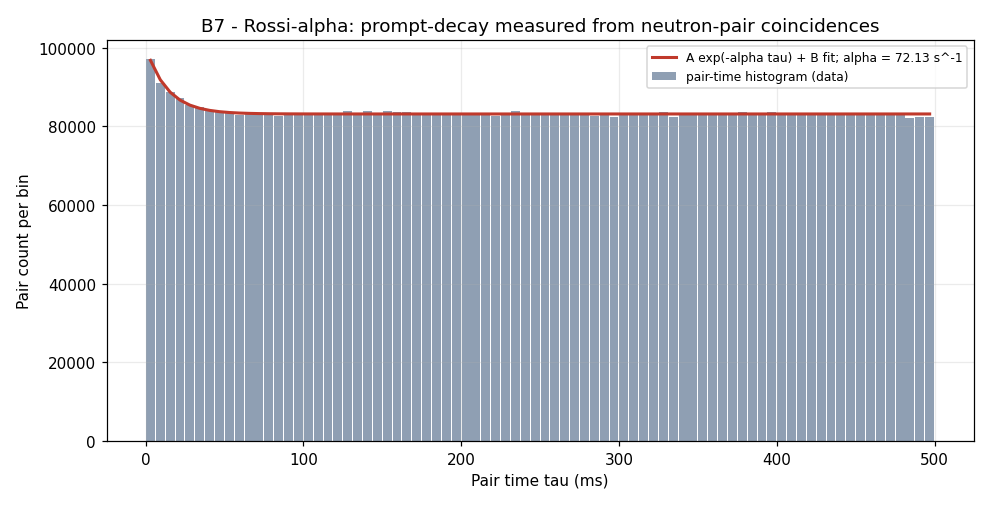
\includegraphics[width=0.92\textwidth]{figures/fig-b7-rossi-alpha}
\end{center}
\textit{Pair-time histogram of a synthetic detector pulse train (51\,635 events
over 200\,s). The exponential-plus-constant fit returns
$\alpha = 72.13$\,s$^{-1}$, within 11\% of the input $\alpha = 65.02$\,s$^{-1}$.}

\section{Toolkit, part 6 --- Feynman-$\alpha$, variance-to-mean as $\alpha$-meter}

Feynman-$\alpha$\footnote{Richard Feynman, \emph{Statistical Behavior of
Neutron Chains}, Los Alamos report LA-591 (1946; declassified 1956). Feynman's
report explains the technique entirely in plain language with two equations;
one wonders whether the modern reactor-physics literature has gained or lost
something by the intervening seventy years of notational sophistication.}
uses the variance-to-mean ratio of \textbf{gated counts}. Partition the pulse
train into consecutive non-overlapping gates of width $T$; count the pulses in
each gate; compute:
\begin{lstlisting}[style=shaddata]
Y(T) = Var(C_T) / Mean(C_T) - 1
\end{lstlisting}

For a pure Poisson process, $Y(T) = 0$. For a reactor pulse train with
multiplet correlation, $Y(T)$ rises from zero and saturates:
\begin{lstlisting}[style=shaddata]
Y(T) = Y_inf * [1 - (1 - exp(-alpha*T)) / (alpha*T)]
\end{lstlisting}

The shape of the rise gives $\alpha$ directly.

\begin{center}
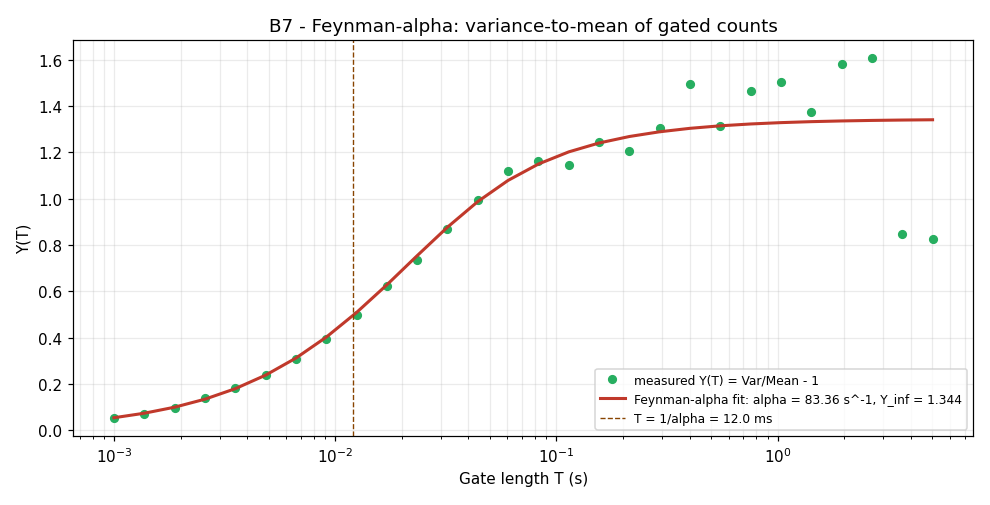
\includegraphics[width=0.92\textwidth]{figures/fig-b7-feynman-alpha}
\end{center}
\textit{$Y(T)$ measured on the same pulse train (28 logarithmically-spaced
gates from 1\,ms to 5\,s). Theoretical Feynman curve (red) fit returns
$\alpha = 83.36$\,s$^{-1}$ and $Y_\infty = 1.344$. Dashed line marks
$T = 1/\alpha$.}

\section{Toolkit, part 7 --- bispectrum, when frequencies talk to each other}

The DFT is a linear operator. It tells you which frequencies are present; it
cannot tell you whether two frequencies are related to each other or merely
coincident. The bispectrum\footnote{Formalised by Brillinger and Rosenblatt in
the 1960s. The reactor-noise community picked it up in the 1980s for detecting
non-linear coupling between neutronic and thermal-hydraulic oscillations in
boiling-water reactors.}
is the third-order generalisation of the power spectrum:
\begin{lstlisting}[style=shaddata]
B(f1, f2) = E[ X(f1) * X(f2) * X*(f1+f2) ]
\end{lstlisting}

For independent or Gaussian processes, $B(f_1, f_2)$ averages to zero
everywhere. For non-Gaussian or quadratically-coupled processes, it has
non-zero off-diagonal structure.

The simulation drives the reactor with two reactivity oscillations at 0.70\,Hz
and 1.10\,Hz plus a deliberately quadratic coupling between them. The DFT shows
three spectral peaks: at 0.70\,Hz, at 1.10\,Hz, and at 1.80\,Hz ($= f_1 + f_2$).
From the DFT alone, you could not tell whether the 1.80\,Hz peak was an
independent third oscillation or the product of a non-linear coupling.

\begin{center}
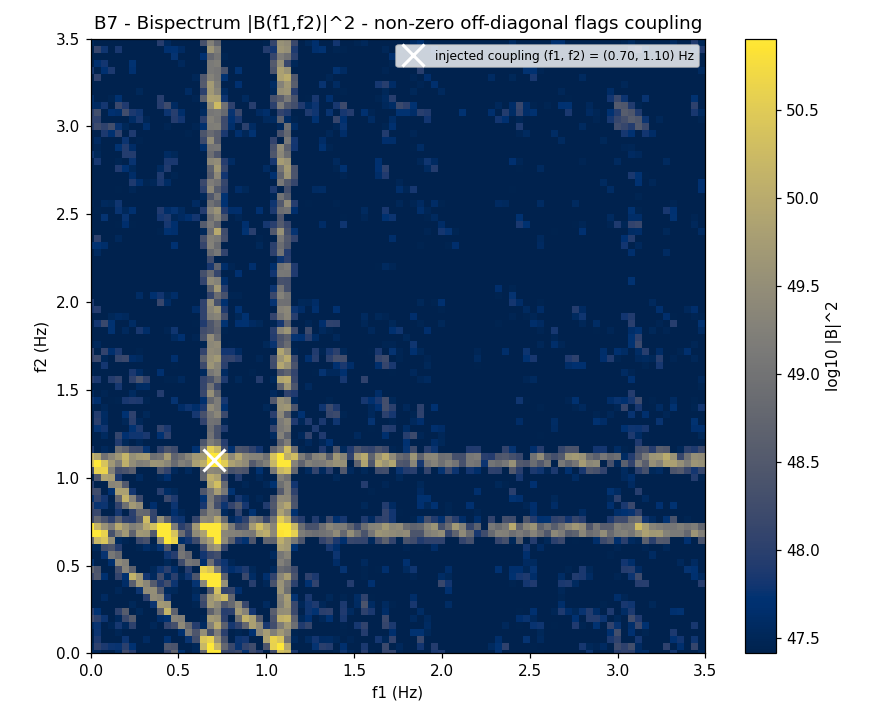
\includegraphics[width=0.92\textwidth]{figures/fig-b7-bispectrum}
\end{center}
\textit{Magnitude-squared bispectrum $|B(f_1, f_2)|^2$ of the coupled reactor
signal (8 Hann-windowed segments, log-colour scale). The bright spot at
(0.70, 1.10)\,Hz (white cross) is the bispectral signature of the quadratic
coupling.}

\section{Toolkit, part 8 --- coherence, when you have two sensors}

The magnitude-squared coherence $\gamma^2(f)$, computed by SciPy's
\texttt{signal.coherence}:
\begin{lstlisting}[style=shaddata]
gamma_sq(f) = |P_xy(f)|^2 / [P_xx(f) * P_yy(f)]
\end{lstlisting}

$\gamma^2$ is bounded between 0 and 1. $\gamma^2 \approx 1$ means detectors
A and B agree at that frequency (common-mode signal dominates); $\gamma^2
\approx 0$ means each detector's own noise dominates.

\begin{center}
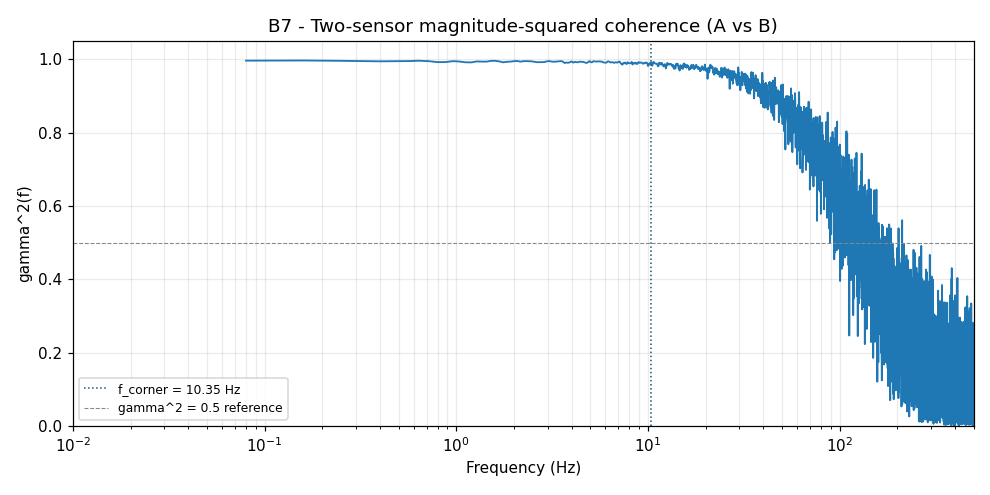
\includegraphics[width=0.92\textwidth]{figures/fig-b7-coherence}
\end{center}
\textit{Magnitude-squared coherence between detector A and detector B
(Welch-style, 16 segments, Hann window). Below the corner frequency,
$\gamma^2 \approx 0.99$ --- the reactor's neutron-field fluctuations dominate.
Above $\sim 50$\,Hz, $\gamma^2$ falls toward 0.5 --- independent
instrument-noise contribution becomes comparable to the reactor signal.}

\section{What we just did}

Twelve figures, one reactor, eight tools.

\medskip
\begin{longtable}{p{0.4cm}p{3.5cm}p{5.5cm}p{3.0cm}}
\toprule
\textbf{\#} & \textbf{Tool} & \textbf{What it told us} & \textbf{Domain} \\
\midrule
\endhead
1 & Time-series view & Reactor wanders $\pm 2$\%. & Time \\
2 & Bare DFT & Lorentzian, corner $\sim 10$\,Hz. & Frequency \\
3 & Welch PSD & Same, $10\times$ less per-bin noise. & Frequency \\
4 & Lorentzian fit & $\alpha = 66.93$\,s$^{-1}$ $\pm 3$\%. & Frequency \\
5 & Bare DFT of transient & Smeared; tells nothing about timing. & Frequency \\
6 & STFT spectrogram & Rod-step localised in time. & Time-frequency \\
7 & Wavelet scalogram & Tighter resolution at high $f$. & Time-frequency \\
8 & Rossi-$\alpha$ & $\alpha = 72.13$\,s$^{-1}$, time-domain. & Time \\
9 & Feynman-$\alpha$ & $\alpha = 83.36$\,s$^{-1}$, gated counts. & Time \\
10 & Bispectrum & Quadratic coupling at (0.70, 1.10)\,Hz. & Freq $\times$ freq \\
11 & Coherence & 99\% common-mode at corner; 50\% at 1\,kHz. & Freq $\times$ sensor \\
\bottomrule
\end{longtable}
\medskip

The pedagogical arc ends here. B1 introduced the DFT as the
instrument-after-the-instrument. B2 through B6 applied it across nine orders
of magnitude in signal strength and six in integration time. B7 closes the arc
by demonstrating, on the canonical reactor-noise problem, where the bare
algorithm stops being sufficient and what you reach for when it does.

The ``and beyond Fourier'' toolkit is not a rejection of Fourier analysis.
Every tool above is \emph{built on} the DFT --- Welch is averaged DFT, the
spectrogram is sliding-window DFT, the wavelet transform is DFT against a
frequency-varying basis, the bispectrum is a higher-order Fourier construct,
and the coherence estimator is a normalised cross-spectrum. The DFT is the
kernel; the toolkit is the kernel applied with care to specific classes of
question.

After this chapter, the reader of the seven-band guide has seen the DFT as a
measurement instrument (B1--B6), as a non-stationary signal probe (B7 STFT
+ CWT), as a non-linear-coupling detector (B7 bispectrum), and as a
multi-sensor agreement test (B7 coherence) --- plus two time-domain methods
that arrive at the same $\alpha$ as the spectral fit and cross-validate it.

Where Shad goes next is into the textbooks --- P\'{a}l, P\'{a}zsit \& P\'{a}l,
and Williams for the reactor-noise canon; Brillinger for higher-order spectra;
Daubechies for wavelets; Welch's original 1967 paper, which is five pages and
still the cleanest presentation of his method.

\section{Try it yourself}

\begin{lstlisting}[style=shaddata]
git clone https://github.com/lege-artis/fourier.git
cd fourier/examples/shad/b7-reactor
pip install numpy scipy matplotlib pywavelets
python main.py
# Renders 12 figures into docs/shad/figures/fig-b7-*.png
# Runtime: ~30 s on a modern laptop.
\end{lstlisting}

All twelve figures regenerate from the same random seed (20260526), so the
numerical claims in this chapter are byte-reproducible across re-runs on any
machine. To change the reactor parameters and watch $\alpha$ and
$f_\mathrm{corner}$ move accordingly, edit the constants at the top of
\texttt{main.py}:

\begin{lstlisting}[style=shadpython]
BETA_I   = np.array([0.000215, 0.001424, 0.001274,
                     0.002568, 0.000748, 0.000273])
LAMBDA_I = np.array([0.0124, 0.0305, 0.111, 0.301, 1.14, 3.01])  # s^-1
GEN_TIME = 1.0e-4   # prompt generation time Lambda
\end{lstlisting}

A fast reactor ($\Lambda \sim 10^{-7}$\,s; metallic fuel, no moderator) gives
$\alpha \sim 10^5$\,s$^{-1}$ and $f_\mathrm{corner} \sim 15$\,kHz. A
graphite-moderated reactor ($\Lambda \sim 10^{-3}$\,s) gives
$\alpha \sim 6.5$\,s$^{-1}$ and $f_\mathrm{corner} \sim 1$\,Hz. The shape of
the Lorentzian is identical across seven orders of magnitude in $\alpha$; only
the corner moves.


% BACK MATTER
% ======================================================================
\appendix

\chapter{Data attribution and licence trail}
\label{ch:dataattr}

\begin{longtable}{p{2.0cm}p{4.5cm}p{3.0cm}p{4.7cm}}
\toprule
\textbf{Slot} & \textbf{Upstream} & \textbf{Licence} & \textbf{Required attribution} \\
\midrule
\endhead
S1 & \texttt{shared/golden-vectors/dft\_n=64.json}, case \texttt{cos1\_plus\_cos2}; in-repo, generated by \texttt{tools/generate\_golden\_vectors.py} & Apache-2.0 / CC-BY-SA-4.0 (project licence stack) & ``lege-artis/fourier golden vectors v0.1.0'' \\
S2a & Wikimedia Commons \texttt{Sine\_wave\_440.ogg} (User:Omegatron) & CC-BY-SA-3.0 & ``Omegatron, Wikimedia Commons, CC-BY-SA-3.0'' \\
S2b & Wikimedia Commons \texttt{Tone\_440Hz.ogg} & CC-BY-SA / CC0 (file-specific) & per-file Wikimedia Commons attribution string \\
S2c & Wikimedia Commons \texttt{Example.ogg} & CC-BY-SA / per-file & per-file Wikimedia Commons attribution string \\
S4 & Wikimedia Commons \texttt{Guitar\_string\_E2.ogg} & CC-BY-SA / per-file & per-file Wikimedia Commons attribution string \\
B1-CSV & \emph{deferred} --- real Rigol/Siglent capture, format ref \cite{rg272996569}, to land in Chapter~\ref{ch:b1} & TBD on capture & TBD on capture \\
S3 & MIT-BIH Arrhythmia Database, record 100, lead MLII; fetched by \texttt{scipy.datasets.electrocardiogram()} \cite{Moody2001,Goldberger2000} & ODbL 1.0 / Open Data Commons & ``Moody \& Mark, MIT-BIH Arrhythmia Database, PhysioNet'' \\
\bottomrule
\end{longtable}

\chapter{Build reproducibility}
\label{ch:build}

\paragraph{Build command.}
\begin{lstlisting}[style=shaddata]
cd docs/shad
./build-pdf.sh
\end{lstlisting}

\paragraph{What \texttt{build-pdf.sh} does.}
\begin{enumerate}[leftmargin=*,itemsep=0pt]
\item Regenerates \texttt{figures/dragon-icon.pdf} from \texttt{dragon-icon.svg} via \texttt{cairosvg}.
\item Runs \texttt{pdflatex} twice (resolves TOC + cross-references).
\item Cleans intermediate artefacts (\texttt{.aux}, \texttt{.log}, \texttt{.out}, \texttt{.toc}).
\item Writes the final PDF as \texttt{docs/shad/shad-guide.pdf}.
\end{enumerate}

\paragraph{Dependencies.} \texttt{texlive-base}, \texttt{texlive-latex-extra},
\texttt{texlive-fonts-recommended}, \texttt{python3-cairosvg}.

% ----------------------------------------------------------------------
% References (manual, no biblatex to keep build single-pass-clean)
% ----------------------------------------------------------------------
\chapter{References}
\begin{thebibliography}{99}
\bibitem{Cooley1965} J.~W. Cooley and J.~W. Tukey, ``An algorithm for the machine calculation of complex Fourier series,'' \emph{Math.\ Comp.}, vol.~19, pp.~297--301, 1965.
\bibitem{Moody2001} G.~B. Moody and R.~G. Mark, ``The impact of the MIT-BIH Arrhythmia Database,'' \emph{IEEE Eng.\ Med.\ Biol.\ Mag.}, vol.~20, no.~3, pp.~45--50, 2001.
\bibitem{Goldberger2000} A.~L. Goldberger \emph{et al.}, ``PhysioBank, PhysioToolkit, and PhysioNet,'' \emph{Circulation}, vol.~101, no.~23, pp.~e215--e220, 2000.
\bibitem{rg272996569} S\'{a}nchez-Olivares et al., ``Raw data file obtained from the oscilloscope,'' ResearchGate figure 272996569 (companion to publication; format used here as canonical layout reference).
\bibitem{PDG2022} R.~L. Workman \emph{et al.} (Particle Data Group), ``Review of Particle Physics,'' \emph{Prog.\ Theor.\ Exp.\ Phys.} 2022, 083C01 (2022).
\bibitem{Rodriguez2018} S. Rodriguez, ``Muon lifetime dataset,'' HU Berlin cosmic-ray laboratory archive, 2018. URL: \url{amor.cms.hu-berlin.de/~rodrigus}.

\bibitem{Skolnik2001} M.~Skolnik, \emph{Introduction to Radar Systems}, 3rd ed., McGraw-Hill, 2001.
\bibitem{Richards2010} M.~Richards, J.~Scheer, W.~Holm (eds.), \emph{Principles of Modern Radar: Basic Principles}, SciTech Publishing, 2010.
\bibitem{Backer1982} D.\,C. Backer \emph{et al.}, ``A millisecond pulsar,'' \emph{Nature} 300, 615--618 (1982).
\bibitem{Manchester2005} R.\,N. Manchester \emph{et al.}, ``The ATNF Pulsar Catalogue,'' \emph{Astron.\ J.} 129, 1993 (2005).
\bibitem{Lorimer2004} D.\,R. Lorimer and M. Kramer, \emph{Handbook of Pulsar Astronomy}, Cambridge University Press, 2004.
\bibitem{Agazie2023} G. Agazie \emph{et al.} (NANOGrav), \emph{Astrophys.\ J.\ Suppl.} 265, 49 (2023).
\bibitem{Taylor1982} J.\,H. Taylor and J.\,M. Weisberg, \emph{Astrophys.\ J.} 253, 908 (1982).
\bibitem{Cohn1960} C.\,E. Cohn, ``A simplified theory of pile noise,'' \emph{Nucl.\ Sci.\ Eng.} \textbf{7}, 472 (1960).
\bibitem{BellGlasstone1970} G.\,I. Bell and S. Glasstone, \emph{Nuclear Reactor Theory}, Van Nostrand Reinhold, New York (1970).
\bibitem{Pal1976} L. P\'{a}l, \emph{Theory of Linear Stochastic Reactor-Kinetic Equations}, Akad\'{e}miai Kiad\'{o}, Budapest (1976).
\bibitem{PazsitPal2008} I. P\'{a}zsit and L. P\'{a}l, \emph{Neutron Fluctuations: A Reference Manual}, Elsevier, Amsterdam (2008).
\bibitem{Williams1974} M.\,M.\,R. Williams, \emph{Random Processes in Nuclear Reactors}, Pergamon, Oxford (1974).
\bibitem{Welch1967} P.\,D. Welch, ``The use of fast Fourier transform for the estimation of power spectra,'' \emph{IEEE Trans.\ Audio Electroacoust.} \textbf{AU-15}, 70 (1967).
\bibitem{Daubechies1992} I. Daubechies, \emph{Ten Lectures on Wavelets}, SIAM (1992).
\bibitem{Hughes2004} H. Hughes, \emph{Spacecraft Attitude Dynamics}, Wiley, 2004.
\bibitem{Landau1976} L.\,D. Landau and E.\,M. Lifshitz, \emph{Mechanics} (Vol.\ I, Course of Theoretical Physics), 3rd ed., Pergamon, 1976.
\bibitem{Goldstein2002} H. Goldstein, C. Poole, J. Safko, \emph{Classical Mechanics}, 3rd ed., Addison-Wesley, 2002.

\end{thebibliography}

\end{document}
